%%%%%%%%%%%%%%%%%%%%%%%%%5
%% abtex2-modelo-trabalho-academico.tex, v<VERSION> laurocesar
%% Copyright 2012-<COPYRIGHT_YEAR> by abnTeX2 group at http://www.abntex.net.br/ 
%%
%% This work may be distributed and/or modified under the
%% conditions of the LaTeX Project Public License, either version 1.3
%% of this license or (at your option) any later version.
%% The latest version of this license is in
%%   http://www.latex-project.org/lppl.txt
%% and version 1.3 or later is part of all distributions of LaTeX
%% version 2005/12/01 or later.
%%
%% This work has the LPPL maintenance status `maintained'.
%% 
%% The Current Maintainer of this work is the abnTeX2 team, led
%% by Lauro César Araujo. Further information are available on 
%% http://www.abntex.net.br/
%%
%% This work consists of the files abntex2-modelo-trabalho-academico.tex,
%% abntex2-modelo-include-comandos and abntex2-modelo-references.bib
%%

% ------------------------------------------------------------------------
% ------------------------------------------------------------------------
% abnTeX2: Modelo de Trabalho Academico (tese de doutorado, dissertacao de
% mestrado e trabalhos monograficos em geral) em conformidade com 
% ABNT NBR 14724:2011: Informacao e documentacao - Trabalhos academicos -
% Apresentacao
% ------------------------------------------------------------------------
% ------------------------------------------------------------------------

\documentclass[
	% -- opções da classe memoir --
	12pt,				% tamanho da fonte
%  openright,			% capítulos começam em pág ímpar (insere página vazia caso preciso)
	twoside,			% para impressão em recto e verso. Oposto a oneside
	a4paper,			% tamanho do papel. 
	% -- opções da classe abntex2 --
	%chapter=TITLE,		% títulos de capítulos convertidos em letras maiúsculas
	%section=TITLE,		% títulos de seções convertidos em letras maiúsculas
	%subsection=TITLE,	% títulos de subseções convertidos em letras maiúsculas
	%subsubsection=TITLE,% títulos de subsubseções convertidos em letras maiúsculas
	% -- opções do pacote babel --
	english,			% idioma adicional para hifenização
	french,				% idioma adicional para hifenização
	spanish,			% idioma adicional para hifenização
	brazil				% o último idioma é o principal do documento
	]{abntex2}

% ---
% Pacotes básicos 
% ---
\usepackage{lmodern}			% Usa a fonte Latin Modern			
\usepackage[T1]{fontenc}		% Selecao de codigos de fonte.
\usepackage[utf8]{inputenc}		% Codificacao do documento (conversão automática dos acentos)
\usepackage{lastpage}			% Usado pela Ficha catalográfica
\usepackage{indentfirst}		% Indenta o primeiro parágrafo de cada seção.
\usepackage{color}				% Controle das cores
\usepackage{graphicx}			% Inclusão de gráficos
\usepackage{microtype} 			% para melhorias de justificação
% ---
		
% ---
% Pacotes adicionais, usados apenas no âmbito do Modelo Canônico do abnteX2
% ---
\usepackage{lipsum}				% para geração de dummy text
% ---

% ---
% Pacotes de citações
% ---
\usepackage[brazilian,hyperpageref]{backref}	 % Paginas com as citações na bibl
\usepackage[alf]{abntex2cite}	% Citações padrão ABNT

\usepackage{geometry}
\geometry{a4paper,left=3cm,right=2cm,top=3cm,bottom=2cm}

% --- 
% CONFIGURAÇÕES DE PACOTES
% --- 

% ---
% Configurações do pacote backref
% Usado sem a opção hyperpageref de backref
\renewcommand{\backrefpagesname}{Citado na(s) página(s):~}
% Texto padrão antes do número das páginas
\renewcommand{\backref}{}
% Define os textos da citação
\renewcommand*{\backrefalt}[4]{
	\ifcase #1 %
		Nenhuma citação no texto.%
	\or
		Citado na página #2.%
	\else
		Citado #1 vezes nas páginas #2.%
	\fi}%
% ---

% ---
% Informações de dados para CAPA e FOLHA DE ROSTO
% ---
\titulo{OTIMIZAÇÃO DO POSICIONAMENTO DE PONTOS DE ACESSO WIRELESS}
\autor{SAMUEL TERRA VIEIRA}
\data{2017}
\local{FORMIGA - MG}
\orientador{Prof.~Msc. Everthon Valadão dos Santos}
\coorientador{}
\instituicao{%
  Instituto Federal de Educação, Ciência e Tecnologia de Minas Gerais -
  Campus Formiga
  \par
  Ciência da Computação
}
\tipotrabalho{Monografia}

% O preambulo deve conter o tipo do trabalho, o objetivo (propósito), 
% o nome da instituição e a área de concentração.
% Esse texto irá compor a Folha de Rosto e Folha de Aprovação.
\preambulo{
Monografia apresentada ao Curso de Ciência da Computação do Instituto
Federal de Educação, Ciência e Tecnologia de Minas Gerais - Campus
Formiga, como requisito parcial para obtenção do grau de Bacharel em
Ciência da Computação.
\newline\textbf{Área de concentração}: Computação.
}%% fim do preambulo




% ---
% Configurações de aparência do PDF final

% alterando o aspecto da cor azul
\definecolor{blue}{RGB}{41,5,195}

% informações do PDF
\makeatletter
\hypersetup{
     	%pagebackref=true,
		pdftitle={\@title}, 
		pdfauthor={\@author},
    	pdfsubject={\imprimirpreambulo},
	    pdfcreator={LaTeX with abnTeX2 and Limarka},
		pdfkeywords={abnt}{latex}{abntex}{abntex2}{trabalho acadêmico}, 
		colorlinks=false,       		% false: boxed links; true: colored links
    	linkcolor=black,          	% color of internal links
    	citecolor=black,        		% color of links to bibliography
    	filecolor=black,      		% color of file links
		urlcolor=black,
		urlcolor=blue,
		bookmarksdepth=4
}
\makeatother
% --- 

% ---
% Possibilita criação de Quadros e Lista de quadros.
% Ver https://github.com/abntex/abntex2/issues/176
%
\newcommand{\quadroname}{Quadro}
\newcommand{\listofquadrosname}{Lista de quadros}

\newfloat[chapter]{quadro}{loq}{\quadroname}
\newlistof{listofquadros}{loq}{\listofquadrosname}
\newlistentry{quadro}{loq}{0}

% configurações para atender às regras da ABNT
\setfloatadjustment{quadro}{\centering}
\counterwithout{quadro}{chapter}
\renewcommand{\cftquadroname}{\quadroname\space} 
\renewcommand*{\cftquadroaftersnum}{\hfill--\hfill}
% ---


% --- 
% Espaçamentos entre linhas e parágrafos 
% --- 

% O tamanho do parágrafo é dado por:
\setlength{\parindent}{1.3cm}

% Controle do espaçamento entre um parágrafo e outro:
\setlength{\parskip}{0.2cm}  % tente também \onelineskip

% ---
% compila o indice
% ---
\makeindex
% ---

%---
% CONFIGURAÇÕES EXTRA DO LIMARKA
%---

% Configura citações de pandoc para 4cm à esquerda (utiliza o ambiente quote)
\renewenvironment{quote}
  {\small\list{}{\rightmargin=0.1cm \leftmargin=4cm}%
   \item\relax}
  {\endlist}

% Para incluir páginas PDF (ficha catalografica e folha de aprovação)
\usepackage[dvipsnames]{xcolor} % http://tex.stackexchange.com/questions/124636/package-xcolor-error-undefined-colors-maroon-royal-blue-when-master-has-pdf
\usepackage{pdfpages}
\usepackage{longtable,ltcaption} % para as tabelas pandoc e quadros ABNT
%\usepackage{floatrow}
%\floatsetup[figure]{capposition=top}


% ---
% BUG: Imagens e tabelas apareciam no meio da página em branco 
% https://github.com/abntex/trabalho-academico-limarka/issues/1
% O código a seguir posta imagens ou tabelas em página em branco no topo, em vez do meio (comportamento padrão)
\makeatletter
\setlength{\@fptop}{5pt} % Set distance from top of page to first float
\makeatother
% ---

% ---
% CUSTOMIZAÇÕES DO USUÁRIO
% ---

\usepackage{latexcustomizacao} % importa customições do usuário.

%%
%% Esse modelo é responsável pela impressão dos seguintes elementos:
%% Capa, Folha de rosto e Ficha catalográfica.


% ----
% Início do documento
% ----
\begin{document}

% Seleciona o idioma do documento (conforme pacotes do babel)
%\selectlanguage{english}
\selectlanguage{brazil}

% Retira espaço extra obsoleto entre as frases.
\frenchspacing 

% ----------------------------------------------------------
% ELEMENTOS PRÉ-TEXTUAIS
% ----------------------------------------------------------
% \pretextual

% ---
% Capa
% ---
\imprimircapa
% ---

% ----------------------------------------------------------
% ELEMENTOS PRÉ-TEXTUAIS
% ----------------------------------------------------------
% \pretextual

% ---
% Folha de rosto: sempre será impressa
% ---

\imprimirfolhaderosto* % (o * indica que haverá a ficha catalográfica)

% ---
% Inserir a ficha catalográfica
% ---
% Provavelmente a biblioteca da sua universidade lhe fornecerá um PDF
% com a ficha catalográfica definitiva após a defesa do trabalho. Quando estiver
% com o documento, salve-o como PDF no diretório do seu projeto e substitua todo
% o conteúdo de implementação deste arquivo pelo comando abaixo:

\begin{fichacatalografica}
    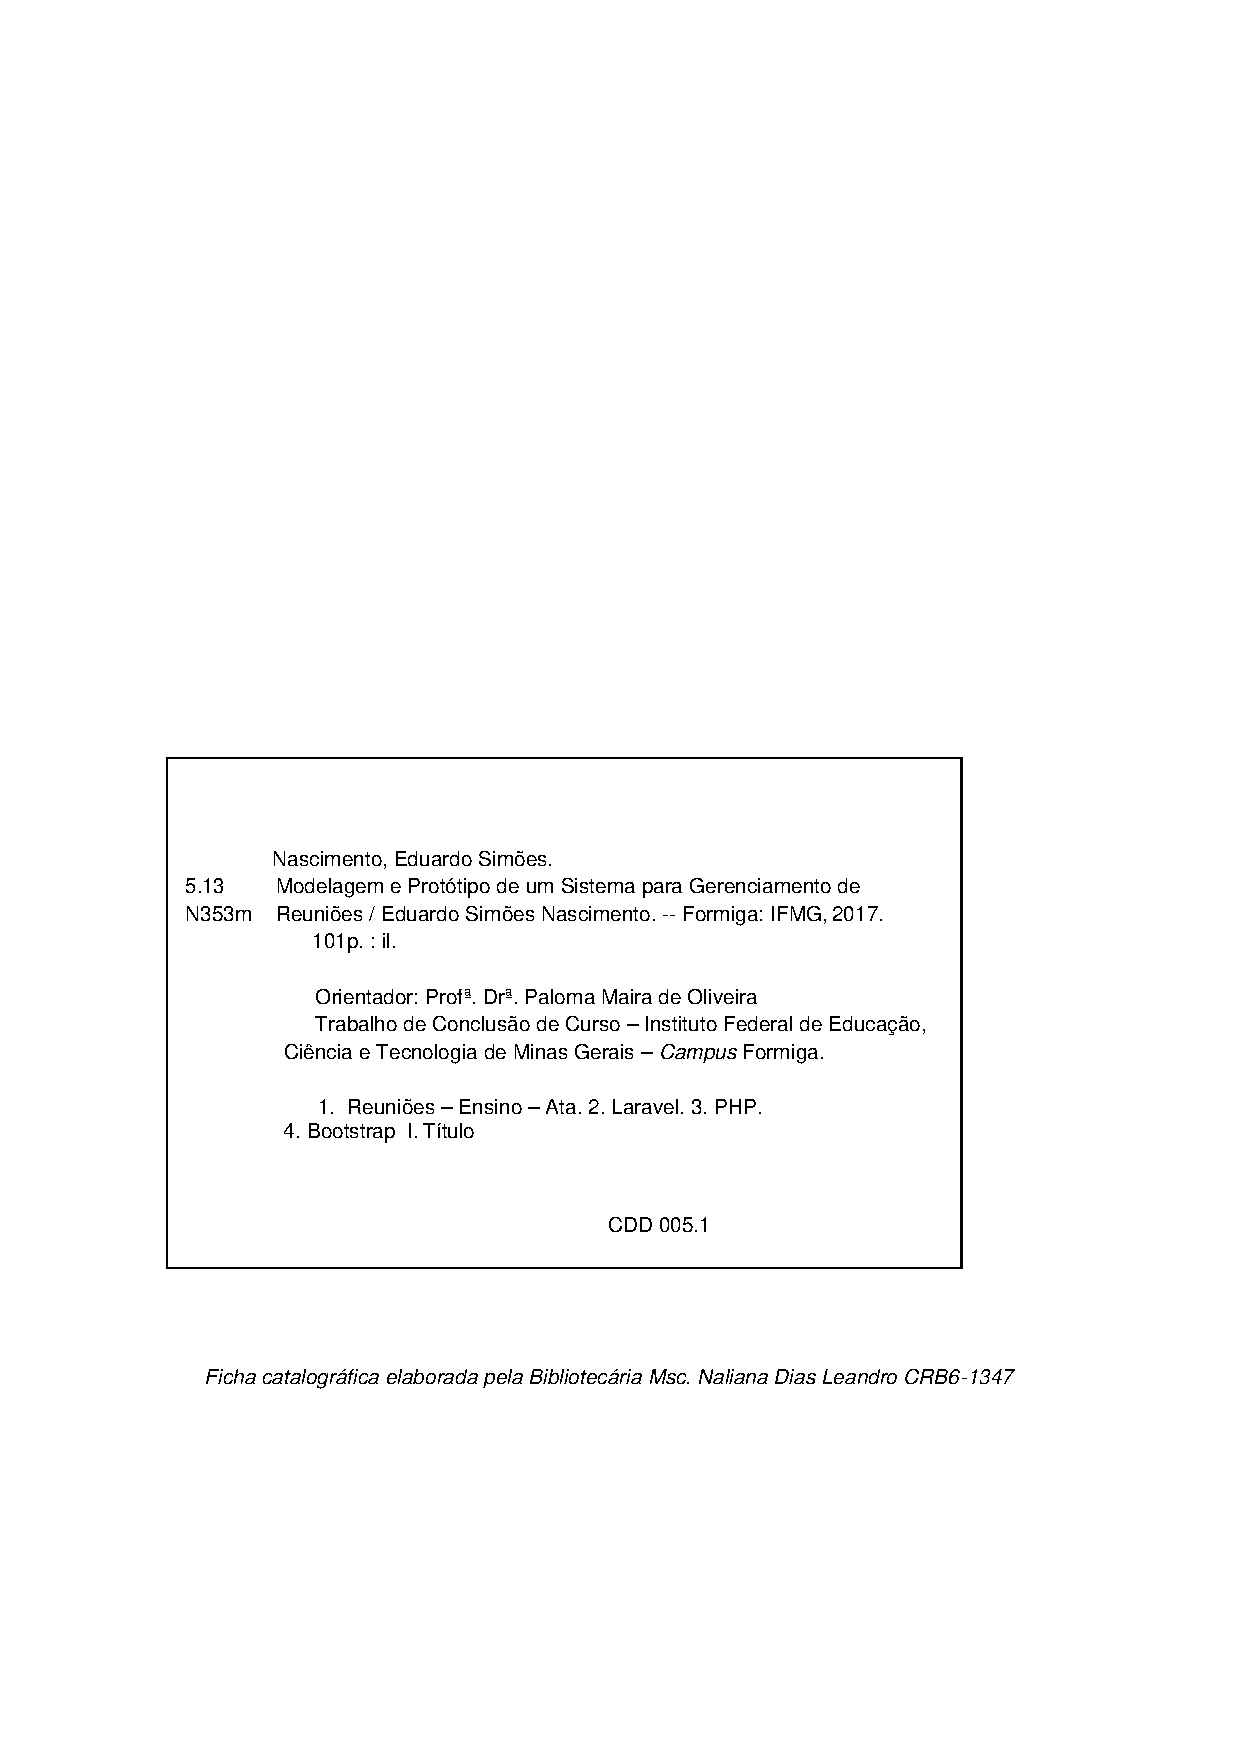
\includepdf{imagens/ficha-catalografica.pdf}
\end{fichacatalografica}

% ---


% ---
% ERRATA: Sem errata
% ---

% ---
% Folha de aprovação incluída
% ---

% Após após aprovação do trabalho a folha deve ser assinada, escaneada e
% incluída como abaixo:
\begin{folhadeaprovacao}
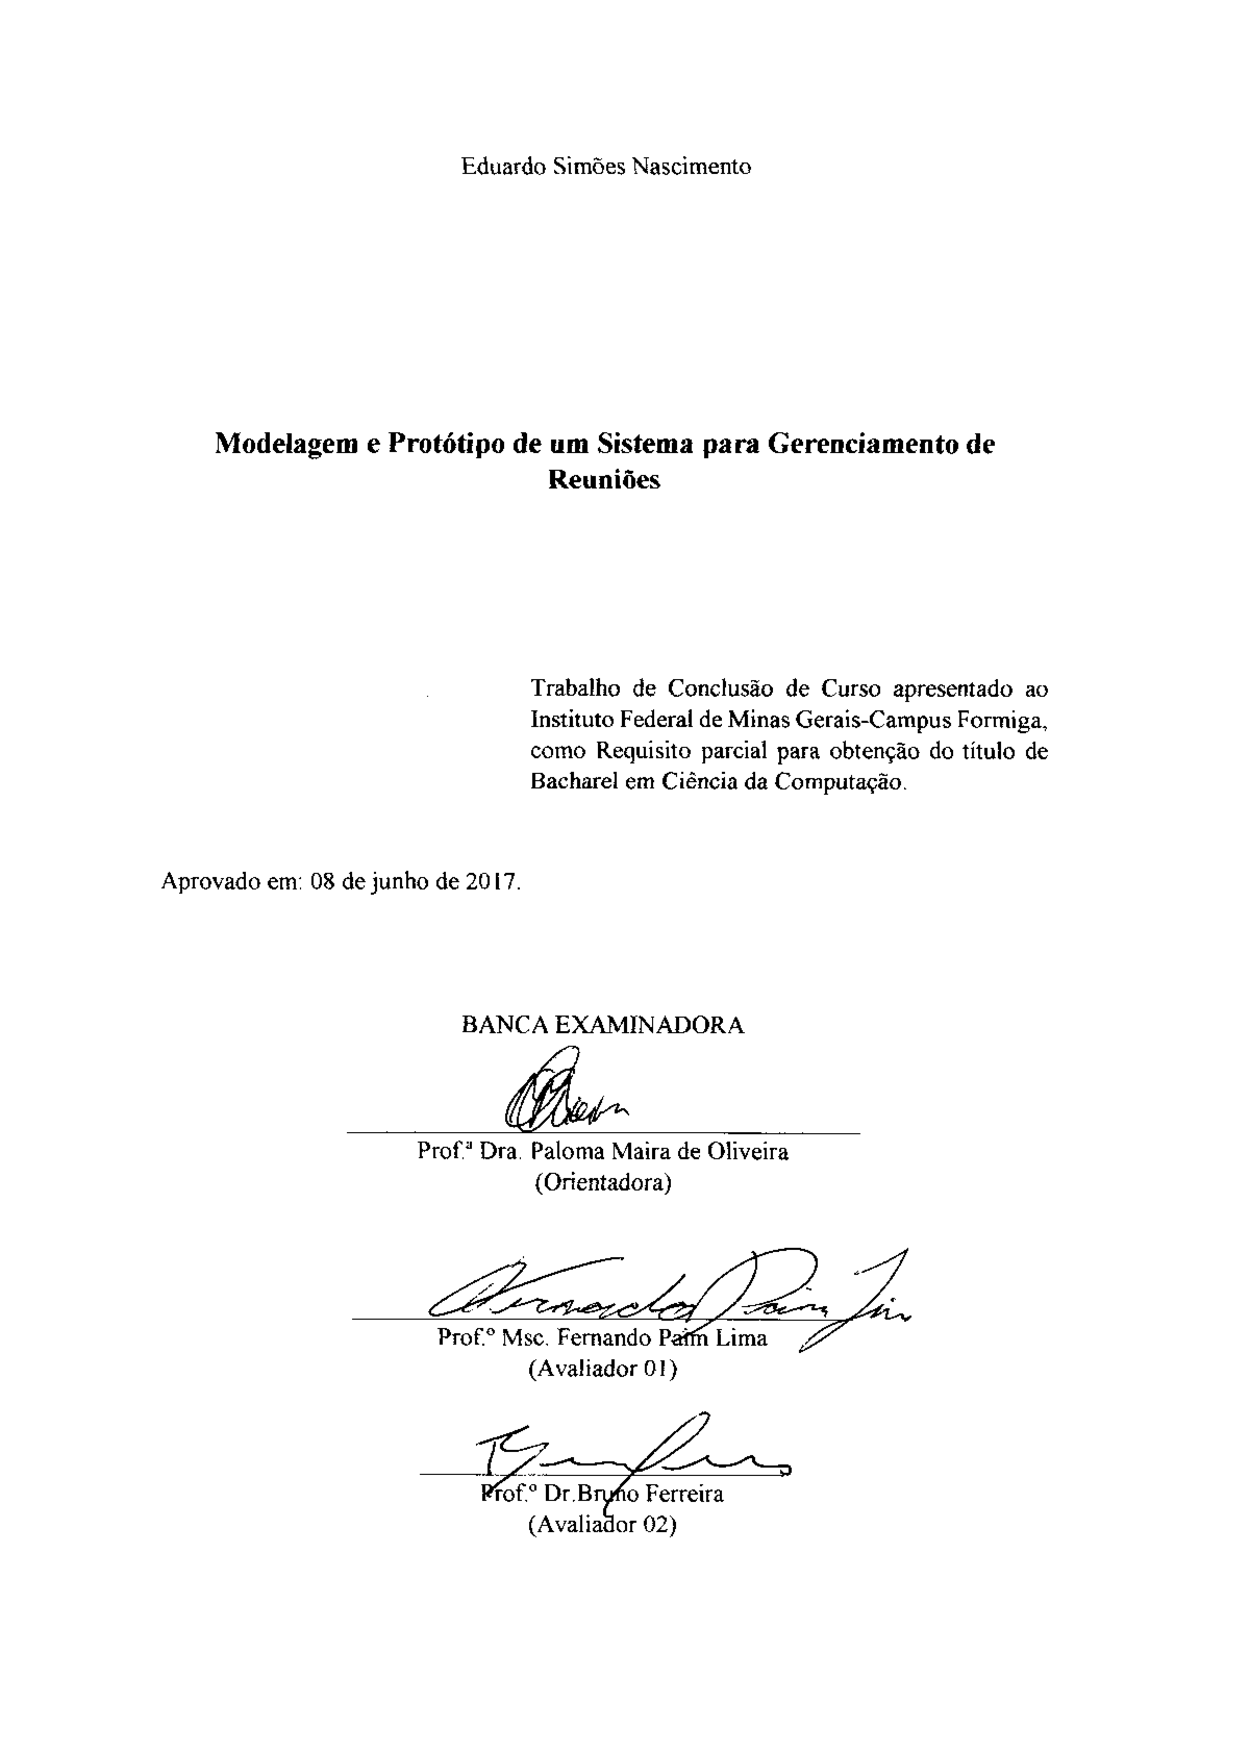
\includepdf{imagens/folha-de-aprovacao-escaneada.pdf}
\end{folhadeaprovacao}

% ---
% Sem Folha de aprovação
% ---
% ---

% ---
% Dedicatória
% ---
% ---
% Agradecimentos
% ---
\begin{agradecimentos}

Agradeço a Deus, pois sem Sua ajuda, direção e o Seu agir em minha vida,
não teria capacidade e o empenho para chegar até aqui; por se fazer
presente até nos momentos em que os desafios foram tão grandes quanto
minha vontade, por me ter dotado de saúde, sabedoria e disposição para
alcançar mais uma etapa em minha vida.

Agradeço aos meus pais que, com toda humildade e simplicidade, me
ensinaram a ser uma pessoa decente, a respeitar e buscar meus sonhos de
forma honesta e dentro do meu tempo, mesmo que seja com muito trabalho
árduo.

Agradeço ao responsável pela parte de TI do campus, Roger Ferreira, e ao
engenheiro civil do campus, Alysson Geraldo, por terem gentilmente
cedido as plantas-baixas. Agradeço ao professor Everthon Valadão, a
paciência e compreensão que teve comigo durante o período em que me
acompanhou e que estivemos juntos realizando este trabalho. Esteve
sempre presente como um grande professor e amigo, sempre se mostrando
comprometido em dar o seu melhor para os alunos.

\end{agradecimentos}
% ---
% ---
% Epígrafe
% ---
\begin{epigrafe}
    \vspace*{\fill}
	\begin{flushright}

  \emph{``Se vi mais longe foi por estar de pé sobre ombros de
  gigantes.''\\
  Isaac Newton}

	\end{flushright}
\end{epigrafe}
% ---

% ---
% Resumo na língua vernácula (obrigatório)
% ---


% resumo em português
\setlength{\absparsep}{18pt} % ajusta o espaçamento dos parágrafos do resumo
\begin{resumo}

  A proposta deste trabalho é desenvolver um software para Wireless AP
  Placement que utilizará modelo(s) da propagação do sinal Wi-Fi de acordo
  com as características físicas do ambiente, aplicando o Simulated
  Annealing como metaheurística para visar ao aprimoramento da cobertura
  de sinal, tendo como caso de uso as dependências do IFMG campus Formiga.
  Tal software fornece um melhor posicionamento dos access points Wi-Fi
  para o ambiente analisado, bem como informa o percentual de cobertura de
  sinal para tal quantidade de APs. O trabalho realizado foi
  disponibilizado de forma gratuita utilizando licença pública geral GNU
  GPL. Ressaltamos que ele possibilita testar disposições de APs sem o
  custo operacional de fisicamente movê-los, de maneira a propor uma
  disposição espacial dos mesmos que forneça uma maior cobertura e
  intensidade de sinal dentro do ambiente simulado. Para trabalhos
  futuros, a fim de se obter resultados que possibilitem uma melhor busca
  pelos pontos de acesso para dois ou mais APs, novas técnicas poderiam
  ser utilizadas para o cálculo da função objetivo da metaheurística.

 \textbf{Palavras-chave}: Wireless. Propagação. Posicionamento. Wi-Fi. Simulated Annealing. CUDA.
\end{resumo}


% ---
% Resumo em língua estrangeira (obrigatório)
% ---

% resumo em inglês
\begin{resumo}[Abstract]
 \begin{otherlanguage*}{english}
   This work aims to develop a software for Wirelless AP Placement that
   will use Wi-Fi signal propagation model (s) according to the physical
   characteristics of the environment, applying the Simulated Annealing as
   a metaheuristic for the improvement of signal coverage, taking as a case
   of use the dependencies of the IFMG - Formiga campus. Such software
   provides a better positioning of the Wi-Fi access points for the
   analyzed environment and informs the percentage of signal coverage for
   such amount of APs. The work was made available free of charge using the
   GNU GPL general public license. We emphasize that it makes it possible
   to test dispositions of APs without the operational cost of physically
   moving them, in order to propose a spatial arrangement of them that
   provides a greater coverage and signal intensity within the simulated
   environment. For future work, in order to obtain results that allow a
   better search for access points for two or more APs, new techniques
   could be used to calculate the objective function of metaheuristics.

   \vspace{\onelineskip}
 
   \noindent 
   \textbf{Keywords}: Wireless. Propagation. Positioning. Wi-Fi. Simulated Annealing. CUDA.
 \end{otherlanguage*}
\end{resumo}


% ---

% ---
% Lista de ilustrações (opcional)
% ---
\pdfbookmark[0]{\listfigurename}{lof}
\listoffigures*
\cleardoublepage


% ---
% inserir lista de quadros
% ---
\pdfbookmark[0]{\listofquadrosname}{loq}
\listofquadros*
\cleardoublepage
% ---

% ---
% Lista de tabelas (opcional)
% ---
\pdfbookmark[0]{\listtablename}{lot}
\listoftables*
\cleardoublepage
% ---

% ---
% Lista de abreviaturas e siglas (opcional)
% ---
\begin{siglas}
  \item[2D] 2 dimensões
  \item[3D] 3 dimensões
  \item[AP] Access Point
  \item[API] Application Programming Interface
  \item[CAD] Computer-aided Design
  \item[CPU] Central Processing UnitHPC High Performance Computing
  \item[CUDA] Compute Unified Device Architecture
  \item[dB] decibel
  \item[dBm] Decibel Miliwatt
  \item[DWG] Drawing
  \item[DXF] Drawing Exchange Format
  \item[EMI] Interferência Eletromagnética
  \item[FOSS] Free Open Source Software
  \item[Gb/s] Gigabits por segundo
  \item[GB] Gigabits
  \item[GHz] Gigahertz
  \item[GNU] Gnu's Not Unix
  \item[GPL] General Public License
  \item[GPS] Global Positioning System
  \item[GPU] Graphics Processing Unit
  \item[IEEE] Institute of Electrical and Electronics Engineers
  \item[ISM] Industrial, Scientific and Medical
  \item[LAN] Local Area Network
  \item[MHz] Megahertz
  \item[PCIe] Peripheral Component Interconnect Express
  \item[RF] Radio Frequency
  \item[SA] Simulated Annealing
  \item[T-R] Transmitter-Receiver
  \item[TI] Tecnologia da Informação
  \item[Wi-Fi] Wireless Fidelity
  \item[WLAN] Wireless Local Area Network
\end{siglas}
% ---

% ---
% Lista de símbolos (opcional): PRESENTE
% ---
\begin{simbolos}
  \item[$ \Delta $] Delta maiúsculo
  \item[$ \mu $] Média aritimética
  \item[$ \delta $] Delta minúsculo
  \item[$ \xi $] Ksi
  \item[$ \sigma $] Sigma
  \item[$ \alpha $] Alpha
  \item[$ \gamma $] Gamma
\end{simbolos}
% ---
% ---
% Sumário
% ---
\pdfbookmark[0]{\contentsname}{toc}
\tableofcontents*
\cleardoublepage
% ---


% ----------------------------------------------------------
% ELEMENTOS TEXTUAIS
% ----------------------------------------------------------
\textual

\chapter{INTRODUÇÃO}\label{introduuxe7uxe3o}

A demanda por disponibilidade e cobertura de redes locais sem fio
(WLAN), seja em ambiente corporativo ou doméstico, tem crescido
vertiginosamente. À medida que o uso de \emph{Wi-Fi} se torna trivial e
cotidiano, suas tecnologias são aperfeiçoadas e os preços dos
equipamentos para acesso sem fio se tornam mais
acessíveis\cite{MARQUES}.

Em um ambiente onde computadores tipicamente realizam a sua comunicação
através de rede local cabeada (LAN), caso seja necessária a realização
de alguma mudança física no ambiente, será inevitável o uso de
arrumações, canaletas ou até obras na estrutura física do prédio.
Conforme ocorrem alterações no ambiente de trabalho, variando desde a
colocação dos móveis e divisórias a mudanças de sala, a limitação
imposta pelos cabos se torna um problema de organização e planejamento
das futuras mudanças. Quando há a necessidade de ampliar a rede para a
acomodação de novos pontos de acesso para telecomunicação, a necessidade
de se estender o atual cabeamento torna-se inconveniente. O obstáculo às
alterações se torna ainda maior quando o ambiente é alguma construção em
que não é viável realizar intervenções na parede (e.g., tombamento ou
estética) para a redistribuição dos cabos, por vezes em edifícios, onde,
sequer, houve planejamento de uma rede cabeada estruturada.

Considerando o acima exposto, é possível observar o quanto é conveniente
o uso de redes sem fio (\emph{wireless}) quando há a necessidade de
ampliar a rede ou implantar, mesmo que temporariamente, o acesso à
internet em alguma determinada área. Apesar da praticidade, não é viável
ter uma rede \emph{wireless} se sua cobertura de sinal não atinge boa
parte da área necessária ou, então, se por mais perto que o ponto de
acesso (AP) \emph{wireless} esteja do computador, não provê uma
qualidade de serviço satisfatória devido a um baixo nível de sinal ou
interferências na mesma frequência do canal.

Isso posto, faz-se necessário um bom planejamento do posicionamento dos
APs \emph{wireless} de maneira a oferecer uma boa cobertura de sinal
onde ouver demanda de conectividade. É importante deixar claro que o
tratamento de colisão de canais como sua interferência de APs próximos
não está dentre os principais objetivos dessa pesquisa e, por
conseguinte, não foi implementado. A proposta deste trabalho é
desenvolver um \emph{software} para \emph{Wireless AP Placement}, que
utilizará modelo(s) da propagação do sinal Wi-Fi de acordo com as
características físicas do ambiente, aplicando metaheurísticas que visem
ao aprimoramento da cobertura de sinal, tendo como caso de uso as
dependências do IFMG \emph{campus} Formiga. Tal \emph{software} indicará
um melhor posicionamento dos \emph{access points Wi-Fi} para o ambiente
analisado.

\section{Justificativa}\label{justificativa}

É importante ressaltar a validade prática deste trabalho a ser
desenvolvido, uma vez que uma grande dúvida dos usuários residenciais e
profissionais de TI é saber qual a melhor localização para o(s) AP(s)
\emph{Wi-Fi}. Alguma vezes, essa questão até passa despercebida para o
usuário (doméstico ou empresarial), resultando em locais sem cobertura
de sinal. Boa parte dos ambientes corporativos e residenciais utilizam
um ou mais pontos de acesso sem fio para prover acesso à rede local e
dela para a internet. Entretanto, dispositivos móveis e computadores
tipicamente não observam uma qualidade satisfatória de sinal do
\emph{access point wireless}. Esse problema pode ocorrer pelo fato do AP
não abranger toda a área necessária ou sofrer atenuações devido às
características do ambiente.

Ademais, redes Wi-Fi podem sofrer interferências externas, tais como
telefones sem fio ou ``babás'' eletrônicas que operem na mesma faixa de
frequência (banda ISM de 2.4 GHz), motores elétricos ou outras redes sem
fio que estejam próximos do AP e irradiem EMI na mesma frequência do
canal utilizado, seja ele na banda de 2.4 GHz (IEEE 802.11 b/g) ou 5.8
GHz (IEEE 802.11 a/ac). Por meio de uma análise do espectro de
radiofrequência (RF) é possível detectar o nível dos sinais e/ou
interferências em determinado local, entretanto, um problema facilmente
observável que pode agravar a baixa qualidade observada no serviço da
rede sem fio é a existência de pontos cegos na cobertura do sinal para
determinado ambiente \cite{RUBINSTEINS}.

Como consequência de toda a atenuação e interferência sofrida, a rede
\emph{wireless} pode ficar inoperante ou dar a impressão de baixo
desempenho. Por parte da maioria dos usuários finais, uma reclamação
comum é a dificuldade de acessar determinado conteúdo e o acesso à rede
parecer ``lento''. De um modo geral, por serem leigos no assunto, muitos
usuários de rede sem fio acabam culpando o provedor de acesso à internet
ou equipe de TI da instituição pela má qualidade do serviço quando, na
verdade, a solução para o problema passaria por uma inspeção no espectro
de sinal do(s) AP(s) \emph{Wi-Fi} (para identificar interferências) e um
melhor posicionamento deste(s) (para maximizar a cobertura do sinal e
reduzir interferências entre APs).

Por fim, até onde pudemos verificar, não há disponível um
\emph{software} livre, gratuito e de código-fonte aberto para
\emph{Wireless AP Placement}, apenas soluções proprietárias, comerciais
e custosas. Isto posto justifica-se o desenvolvimento da ferramenta
proposta neste trabalho.

\section{Objetivos}\label{objetivos}

Após a contextualização do objeto de estudo deste trabalho e sua
importância, sintetiza-se aqui seu objeto primário: projetar e
implementar um \emph{software} para planejamento do posicionamento dos
APs (\emph{Wireless AP Placement}), que receba como entrada uma
representação do ambiente e informações dos APs disponíveis, realize
simulações de propagação dos sinais (considerando as características do
ambiente) para os posicionamentos de APs propostos por meta-heurística
que vise maximizar a cobertura do sinal Wi-Fi tendo, como caso de uso,
as dependências do IFMG campus Formiga. São objetivos secundários e mais
específicos os seguintes tópicos:

\begin{itemize}
\item
  Construir um modelo das dependências do IFMG campus Formiga, a partir
  da representação do ambiente fornecida ao software,
  e.g.~planta(s)-baixa(s);
\item
  Simular a propagação do sinal wireless de APs Wi-Fi através das
  dependências do campus Formiga, seguindo modelos de propagação de
  sinais sem fio;
\item
  Utilizar metaheurística computacional para propor/verificar, via
  simulação, novas localizações para os APs Wi-Fi, visando maximizar a
  cobertura do sinal no campus (dentre outros fatores);
\item
  Fornecer, ao final, uma solução proposta para o novo posicionamento
  dos APs Wi-Fi, se possível, auxiliada por algum método de visualização
  da cobertura do sinal wireless no ambiente;
\item
  Disponibilizar o software de maneira livre e de código-fonte aberto
  (FOSS), distribuindo-o por meio de alguma licença que proteja a
  autoria do mesmo (e.g., Licença Pública Geral GNU --- GPL).
\end{itemize}

\chapter{FUNDAMENTAÇÃO TEÓRICA}\label{fundamentauxe7uxe3o-teuxf3rica}

No levantamento do referencial bibliográfico realizado, observamos um
vasto número de trabalhos que tratam sobre a otimização do
posicionamento de pontos de acesso \emph{wireless}. Utilizaremos, como
principais fundamentações teóricas deste projeto, o trabalho de Batitti,
Brunato e Delai: \emph{Optimal Wireless Access Point Placement for
Location-Dependent Services} e a obra \emph{Comunicações sem fio -
Princípios e Práticas}, de Theodore S. Rappaport.

\section{\texorpdfstring{\emph{Wireless AP
Placement}}{Wireless AP Placement}}\label{wireless-ap-placement}

De acordo com o trabalho publicado por Battiti, Brunato e Delai
\cite{BATTITI}, ``\emph{Optimal Wireless Access Point Placement for
Location-Dependent Services}'', vários grupos de pesquisadores
independentes têm proposto métodos para fazer estimativa a respeito da
posição do usuário \cite{DALSSOTO}, com base na intensidade dos sinais
de rádio recebidos de múltiplos APs \cite{NAJNUDEL}. Partindo desta
distinta aplicação, os pesquisadores propõem uma nova abordagem para o
AP \emph{Placement}, pois consideram que a localização ``é um importante
parâmetro que pode ser usado para determinar o comportamento do
sistema'' \cite[p. 1]{BATTITI}. Desse modo, a proposta deste TCC, que
utilizará um modelo de propagação do sinal Wi-Fi em uma simulação do
ambiente do IFMG \emph{campus} Formiga é, mais uma vez, justificada pela
necessidade de se ter um software livre e gratuito para \emph{Wireless
AP Placement}, que indique um melhor posicionamento dos \emph{access
points Wi-Fi}.

\section{Tecnologias Wi-Fi ( WLANs IEEE 802.11
)}\label{tecnologias-wi-fi-wlans-ieee-802.11}

Quando se trata de redes \emph{wireless}, é imprescindível dizer que,
com o estabelecimento da família de padrões IEEE 802.11, se tornou
possível a compatibilidade entre diferentes marcas de fabricantes de APs
\emph{wireless} e dispositivos móveis. De acordo com Franciscatti,

\begin{citacao}
    As redes *wireless* utilizam freqüências de rádio para se comunicar
    havendo necessidade de uma padronização dos equipamentos sem fio por
    existir vários fabricantes. Não havia uma padronização dessa tecnologia
    causando, assim, a impossibilidade de comunicação de dispositivos de
    redes sem fio de outros fabricantes. Assim o *Institute of Electrical
    and Electronics \[Engineers\]* (IEEE) formou um grupo de trabalho com o
    objetivo de definir os padrões de uso em redes sem fio, denominado
    802.11. \apud{FRANCISCATTI}{BOF}
\end{citacao}

Desta forma, após a padronização definida pela IEEE, alguns padrões para
WLAN foram estabelecidos \cite{RIVERA,BANERJI}, como:

\begin{itemize}
\item
  \textbf{IEEE 802.11a:} Definido em setembro 1999, operando na
  frequência de 5 GHz, uma largura de banda de 20 MHz, taxa de
  transmissão de até 54 Mbit/s e podendo ter um alcance de 35 metros
  \emph{indoor} e até 5 quilômetros \emph{outdoor};
\item
  \textbf{IEEE 802.11b:} Definido em setembro 1999, operando com uma
  frequência de 2.4 GHz, uma largura de banda de 22 MHz, taxa de
  transmissão de até 11 Mbit/s e com alcance de 35 metros \emph{indoor}
  e 140 metros \emph{outdoor};
\item
  \textbf{IEEE 802.11g:} Definido em junho de 2003, operando com uma
  frequência de 2.4 GHz, utilizando uma largura de banda de 20 MHz, com
  uma taxa de transmissão de até 54 Mbit/s e com um alcance de 38 metros
  \emph{indoor} e 140 metros \emph{outdoor};
\item
  \textbf{IEEE 802.11n:} Definido em outubro de 2009, operando com uma
  frequência de 2.4 GHz (802.11a) e 5 GHz (802.11g), com uma taxa de
  transmissão de até 72.2 Mbit/s utilizando uma largura de banda de 20
  MHz e uma taxa de transmissão de até 150 Mbit/s com uma banda de 40
  MHz, permitindo múltiplos fluxos espectrais (MIMO). O alcance vai de
  70 metros \emph{indoor} e 250 metros \emph{outdoor};
\item
  \textbf{IEEE 802.11ac:} Definido em dezembro de 2013, operando com uma
  frequência de 5 GHz, utilizando uma largura de banda que vai de 20 MHz
  até 160 MHz, com uma taxa de transmissão de 87.6 Mbit/s até até 866.7
  Mbit/s, também com uso de MIMO.
\end{itemize}

Considerando os padrões supracitados, iremos focar especificamente na
penetração dos sinais \emph{Wi-Fi} na estrutura dos edifícios (paredes,
andares).

\section{Propagação de sinais de
rádio}\label{propagauxe7uxe3o-de-sinais-de-ruxe1dio}

O sinal Wi-Fi produzido pelo \emph{access point} nada mais é, de um modo
simplista, que uma onda de rádio que se propaga no espaço. De acordo com
Rappaport,

\begin{citacao}
    Os mecanismos por trás da propagação da onda eletromagnética são diversos, mas geralmente podem ser atribuídos a reflexão, difração e dispersão. (...) Devido a múltiplas reflexões de vários objetos, as ondas eletromagnéticas trafegam por diferentes caminhos de tamanhos variados. A interação entre essas ondas causa uma distorção de caminhos múltiplos em um local específico, e as intensidades das ondas diminui à medida que a distância entre transmissor e receptor aumenta. \cite[p. 72]{RAPPAPORT}
    
\end{citacao}

Por ser uma onda eletromagnética, a onda do sinal \emph{Wi-Fi} como
descrito por Torlak, apresenta tal comportamento, sofrendo reflexão,
difração e dispersão \cite{TORLAK}. Outro aspecto que deve ser abordado
acerca da onda do sinal \emph{Wi-Fi} é a diferença entre modelos de
propagação de larga escala (perdas) e pequena escala (atenuação). Os
modelos de propagação em larga escala são caracterizados pela
intensidade do sinal para grandes distâncias de separação do transmissor
e receptor (podendo variar de várias centenas ou milhares de metros),
enquanto modelos de propagação em pequena escala são caracterizados
pelas flutuações rápidas do sinal recebidos para distâncias muito curtas
(variando de alguns comprimentos de onda ou durações de segundos)
\cite[p. 72]{RAPPAPORT}.

Rappaport define três modelos básicos de propagação que são usados para
a previsão da intensidade do sinal recebido a determinada distância do
transmissor, numa larga escala. O modelo de propagação no espaço livre
(\emph{Friis}) é utilizado quando transmissor e receptor possuem uma
linha de visão desobstruída, ou seja, não há obstáculos entre eles que
interrompam ou alterem o caminho da transmissão do sinal. O modelo de
propagação no espaço livre oferece uma noção da ordem de magnitude do
sinal recebido, mas é demasiado otimista pois raramente há um único
caminho entre a antena transmissora e a antena receptora: em situações
reais, haverá reflexão do sinal no solo. Para grandes distâncias e
antenas altas, o modelo de reflexão no solo é razoavelmente preciso para
prever a intensidade do sinal recebido. Esse modelo é baseado na ótica
geométrica e considera o caminho direto e o caminho refletido (modelo de
dois raios), que muitas vezes é no solo. E, por fim, temos o modelo de
difração (por gume de faca) que torna possível propagar os sinais de
rádio através de obstruções, bem como ao redor da superfície da terra,
além do horizonte. Contudo, a força do campo recebido diminui
rapidamente quando o receptor se aproxima do obstáculo em direção à
região obstruída (sombra), porém, o campo de difração ainda existe e
normalmente tem força suficiente para produzir um sinal útil
\cite[p. 72-83]{RAPPAPORT}.

A propagação no interior é dominada pelos mesmos mecanismos (reflexão,
difração e dispersão), porém as condições são muito variáveis, podendo
variar, por exemplo, até mesmo se as portas e janelas estiverem fechadas
ou dependendo do local onde as antenas são montadas. Dentro do mesmo
contexto, existem várias características físicas e elétricas que podem
influenciar na propagação do sinal, como qual o tipo de ambiente
(escritório ou casa) e de que é feita a construção (madeira, tijolo,
concreto ou até ferragem). Durante a propagação, pode também ocorrer a
perda do sinal entre andares de um edifício, obedecendo à lei de
potência da distância, a qual leva em consideração o tipo de prédio,
arredores e uma variável aleatória normal que representa o desvio padrão
\cite[p. 104-108]{RAPPAPORT}.

\section{Modelos de propagação}\label{modelos-de-propagauxe7uxe3o}

Quando se deseja realizar um bom desempenho e planejamento da cobertura
do espectro Wi-Fi, é indispensável o conhecimento do meio de transmissão
e qual modelo se deve usar para obter um resultado mais realista. Em
sistemas \emph{wireless} o meio de propagação utilizado é o canal de
rádio, de forma que as características e efeitos sobre todas as
informações trafegadas são de uma natureza complexa, fazendo com que
medições empíricas sejam de suma importância. Com as medições é possível
ver como é o comportamento de modelos em pequena e larga escala, além de
ser possível determinar a variação da potência do sinal devido ao
movimento de pessoas no ambiente ou atingir obstáculos fixos, como
paredes, pisos, vidros, móveis, dentre outros.

Então, se faz necessário uma boa escolha de quais modelos de propagação
utilizar quando se quer obter uma boa representação do espectro e que ao
mesmo tempo esteja condizente com a realidade. Quanto maior for a
precisão desejada, mais detalhes sobre o ambiente de propagação devem
ser modelados. Nesta seção serão comentados sucintamente sete modelos
que foram estudados para a realização deste trabalho.

\subsection{\texorpdfstring{Propagação no espaço livre (modelo de
\emph{Friis})}{Propagação no espaço livre (modelo de Friis)}}\label{sec:friis}

O modelo \emph{Friis free-space path loss} ou geralmente tratado como
modelo de propagação no espaço livre de Friis é usado para prever a
intensidade do sinal recebido quando a antena transmissora e a antena
receptora possuem um caminho de linha de visão limpo, ou seja, um
caminho desobstruído de qualquer objeto ou edificação \cite{LUO}. Tal
modelo é em geral usado em sistemas de comunicação por satélite e em
enlaces de rádio de microondas com linha de visão. Assim como os modelos
\emph{outdoor}, o modelo de propagação no espaço livre de Friis,
pressupõe que a potência recebida diminui com uma função da distância
entre a antena transmissora e a antena receptora elevada a alguma
potência, ou seja, uma função da lei de potência. A potência recebida
através do espaço livre pela antena receptora separada da antena
transmissora por uma distância \(d\) pode ser calculada pela seguinte
equação:

\begin{equation}
P_{r}(d)= \frac{P_{t}G_{t}G_{r}\lambda^{2}}{(4\pi)^{2}d^{2}L}
\end{equation}

sendo:

\begin{itemize}
\item
  \(P_{t}\) a potência transmitida;
\item
  \(P_{r}(d)\) a potência recebida na distância \(d\);
\item
  \(G_{t}\) é o ganho da antena transmissora;
\item
  \(G_{r}\) é o ganho da antena receptora;
\item
  \(d\) é a distância de separação das antenas;
\item
  \(L\) é o fator de perda (\(L\geq1\)), \(L = 1\) indica nenhuma perda
  no hardware do sistema;
\item
  \(\lambda\) é o comprimento de onda dado em metros.
\end{itemize}

O modelo de espaço livre de \emph{Friis} é apenas uma previsão válida
para uma potência recebida para uma distância \(d\) de separação entre
as antenas. O campo distante que é criado entre as antenas pode ser
chamado de região de \emph{Fraunhofer}, onde essa região é definida como
uma região além da distância de campo distante \(d_{f}\) , que está
diretamente relacionada com a maior dimensão linear \(D\) de abertura da
antena transmissora e com o comprimento de onda da portadora (antena
receptora) \cite{RAPPAPORT}. Tal distância de \emph{Fraunhofer} pode ser
calculada pela seguinte fórmula:

\begin{equation}
    d_{f} =  \frac{2D^{2}}{\lambda}
\end{equation}

O cálculo da potência recebida tem uma falha quando a distância é zero.
Por este motivo, modelos de propagação em larga escala utilizam uma
distância próxima, \(d_{0}\), com um ponto de referência de potência
conhecido. A potência recebida, \(P_{r}(d)\), em qualquer distância que
a distância \(d\) seja maior que zero, pode estar relacionada com a
potência recebida no ponto de referência \(d_{0}\) \cite{RAPPAPORT}. A
equação que calcula a potência recebida pode ser vista abaixo utilizando
uma distância maior que \(d_{0}\):

\begin{equation}
    P_{r}(d) = P_{r}(d_{0})(\frac{d_{0}}{d})^{2}
\end{equation}

O valor da distância de referência \(d_{0}\) em sistemas práticos em
antenas de baixo ganho, entre 1 e 2 GHz, normalmente é utilizado com
sendo 1 metro em ambientes internos (\emph{indoor}) e 100 metros ou 1
quilômetro para ambientes externos (\emph{outdoor}), de forma que o
resultado obtido pelas equações anteriores são múltiplos de 10, tornando
os cálculos de perda de caminho fácies em unidade de \(dB\).

\subsection{\texorpdfstring{\emph{Two-rays ground
reflection}}{Two-rays ground reflection}}\label{sec:two_rays}

O modelo \emph{Two-rays ground reflection} é um modelo de propagação de
rádio que prevê as perdas de trajetória entre uma antena transmissora e
uma antena receptora. Em geral, as duas antenas têm altura diferente e
raramente possuem uma linha direta\cite{LUO}. O sinal é recebido de duas
formas: por LOS (linha de visão) e o por \emph{multipath} (multicaminho)
formado predominantemente por uma única onda refletida no solo.

Quando a distância entre as antenas é menor do que a altura da antena
transmissora, duas ondas são adicionadas de forma positiva para gerar
maior potência e, à medida que a distância aumenta, essas ondas se somam
de forma construtiva e destrutiva, proporcionando regiões de exaustão e
decaimento à medida que a distância aumenta além da distância crítica ou
primeira zona de Fresnel, a potência cai proporcionalmente quatro vezes
o inverso da potência da distância. Essa é uma perda no caminho muito
mais rápida do que é experimentada no \emph{Friis free-space path loss
model} (espaço livre de Friis).

Quando se tem valores muito altos para a distância, pode-se notar que a
potência recebida e a perda no caminho se tornam independentes da
frequência \cite{RAPPAPORT}. O modelo de reflexão de dois raios é uma
formulação matemática de um tipo de interferência \emph{multipath}
quando a interferência é considerada como consistindo em dois caminhos:
\textbf{(I)} do transmissor ao receptor diretamente, \textbf{(II)} do
transmissor, refletido fora do chão, para o receptor.

A potência recebida a uma distância d do transmissor para o modelo
\emph{Two-rays ground reflection model} pode ser expressa como:

\begin{equation}
    P_{r}(d) = P_{t}G_{t}G_{r}\frac{h^{2}_{t}h^{2}_{r}}{d^{4}}
\end{equation}

sendo:

\begin{itemize}
\item
  \(P_{r}(d)\) a potência recebida com distância \(d\);
\item
  \(P_{t}\) a potência transmitida;
\item
  \(G_{r}\) o ganho da antena receptora;
\item
  \(G_{t}\) o ganho da antena transmissora;
\item
  \(h_{t}\) a altura da antena transmissora;
\item
  \(h_{r}\) a altura da antena receptora;
\item
  \(d\) a distância do transmissor.
\end{itemize}

A perda do caminho para o modelo \emph{Two-rays ground reflection model}
pode ser expressa em \(dB\) com a equação abaixo:

\begin{equation}
PL(dB) = 40 log d -(10 log G_{t} + 10 log G_{r} + 20 log h_{t} + 20 log h_{r})
\end{equation}

\subsection{\texorpdfstring{\emph{Log-distance}}{Log-distance}}\label{sec:log_distance}

O modelo \emph{Log distance path loss} é um modelo genérico e uma
extensão do modelo de espaço livre de Friis. Ele é usado para prever a
perda de propagação para uma ampla gama de ambientes, enquanto que o
modelo Friis é restrito ao caminho desobstruído entre o transmissor e o
receptor \cite{LUO}.

O principal critério ou característica deste modelo é considerar que a
perda no caminho é logaritmicamente dependente da distância. Logo a
perda no caminho calculada com uma distância \(d\) entre um transmissor
e receptor (geralmente dado em quilômetros) . Na região mais distante do
transmissor (onde \(d \geq df\)), se \(PL(d_{0})\) é a perda de percurso
medida em \(dB\) a uma distância \(d_{0}\) do transmissor, então a perda
do caminho (a perda na potência do sinal em \(dB\) quando se desloca de
distância \(d_{0}\) a \(d\)) a uma distância arbitrária \(d > d_{0}\) é
dada pela fórmula:

\begin{equation}
PL(d) = PL(d_{0}) + 10 \cdot n \cdot log(\frac{d_{0}}{d})
\end{equation}

sendo:

\begin{itemize}
\item
  \(d\) é a distância dada em quilômetros em todos os caso;
\item
  \(d_{0}\) é a distância inicial de referência;
\item
  \(PL(d)\) é a perda no caminho para a distância \(d\);
\item
  \(PL(d_{0})\) é um valor de perda de caminho para uma distância de
  referência;
\item
  \(n\) é o expoente de propagação e indica a taxa na qual a perda de
  caminho aumenta com a distância \cite{MATHURANATHAN}.
\end{itemize}

Geralmente, para modelar ambientes reais, os efeitos \emph{shadowing}
(de sombreamento) não podem ser negligenciados. Se os efeitos de
sombreamento forem deixados de lado, a perda do caminho, quando
representada em um gráfico que representa a potência recebida e a
distância, é simplesmente uma linha reta. Para adicionar um efeito de
sombreamento e deixar o resultado final mais próximo da realizada, uma
variável aleatória Gaussiana de média zero com desvio padrão \(\sigma\)
é adicionada à equação. A perda real do caminho ainda pode variar devido
a outros fatores, assim como os efeitos de reflexão, difração e
dispersão. Assim, o expoente da perda de caminho (a literatura define
alguns em ambientes diferentes) e o desvio padrão da variável aleatória
escolhida, devem ser bem conhecidos para uma boa modelagem da perda.

\subsection{\texorpdfstring{\emph{One-slope}}{One-slope}}\label{sec:one_slope}

O modelo \emph{One-slope} é classificado como sendo um modelo empírico e
assume que a perda no caminho dada em \(dBm\) é linearmente na distância
logarítmica da distância \(d\) entre o transmissor e receptor
\cite{LUO}:

\begin{equation}
PL(d) = L_{0} + 10 \cdot n \cdot log(d)
\end{equation}

onde:

\begin{itemize}
\item
  \(d\) é a distância entre transmissor e receptor;
\item
  \(PL(d)\) é a perda no caminho para a distância \(d\);
\item
  \(L_{0}\) é a perda no caminho calculado em uma distância de 1 metro;
\item
  \(n\) é o expoente de perda no caminho.
\end{itemize}

Claramente, este modelo baseia-se na perda do espaço livre e visa
incluir todas as perdas devido a vários mecanismos de propagação pelo
caminho usando um expoente \(n\) de perda. Por ser um modelo simples, se
torna muito fácil de realizar sua implementação, mas se usado de forma
única pode levar a grandes erros em ambientes internos, pois é possível
que um grande números de objetos interfiram nos mecanismos de
propagação, ou seja, não será possível obter um resultado com uma
precisão próxima da realidade.

\subsection{\texorpdfstring{\emph{Wall and floor
factor}}{Wall and floor factor}}\label{sec:wall_floor}

O modelo \emph{Wall and floor factor} leva em conta a absorção em
paredes e pavimentos e geralmente é usado em ambientes internos e
considera a perda no espaço livre \cite{LUO, RAPPAPORT}. Ele se resume
basicamente na perda no espaço livre de um ambiente interno somado com
uma perda adicional relacionada a cada piso atravessado e o número de
paredes interceptadas em uma linha direta entre o transmissor e
receptor.

Segundo Xie, este modelo de propagação tem um desempenho melhor que o
modelo \emph{One-slope}, uma vez que proporciona mais graus de liberdade
na consideração de obstáculos \cite{XIE}. A perda no caminho utilizando
o modelo de propagação \emph{wall and floor factor} pode ser calculada
pela seguinte equação:

\begin{equation}
    PL(d) = L_{1} + 20 \cdot log(d) + n_{f} \cdot L_{f} + n_{w} \cdot L_{w}
\end{equation}

sendo:

\begin{itemize}
\item
  \(d\) é a distância entre transmissor e receptor;
\item
  \(PL(d)\) é a perda no caminho para a distância \(d\);
\item
  \(L_{1}\) é a perda no caminho calculado em uma distância de 1 metro;
\item
  \(n\) é o expoente de perda no caminho;
\item
  \(L_{f}\) e \(L_{w}\) são respectivamente perdas causadas pela
  penetração no piso e nas paredes;
\item
  \(n_{f}\) e \(n_{w}\) são respectivamente os números de pisos e de
  paredes.
\end{itemize}

\subsection{\texorpdfstring{\emph{Log-normal
fading}}{Log-normal fading}}\label{sec:log_normal_fading}

Este modelo de propagação estatístico provê uma estimativa aproximada do
que representa a perda no caminho como uma função da distância e outros
parâmetros como a frequência e a altura da antena \cite{BUDGETS}. Desta
forma é possível obter uma previsão da qualidade da intensidade do sinal
quando aumentamos a distância entre o transmissor e receptor. Vale
ressaltar que, para se obter uma representação mais realista da perda do
sinal, é necessária uma grande coleta de dados empíricos.

\begin{equation}
    f(x; \mu; \sigma) = \frac{1}{x \sigma \sqrt{2 \pi}} exp[-\frac{(ln(x) - \mu)^{2}}{2 \sigma^{2}}]
\end{equation}

Uma possível explicação para o motivo pelo qual este modelo utiliza uma
distribuição \emph{log-normal} é que, para cada caminho há muitos
fatores que contribuem com a perda do sinal, incluindo a combinação de
perda no espaço livre, difrações, reflexões, interferências de
equipamentos, dentre outros motivos. Para cada uma dessas perdas, é
utilizada uma variável aleatória que a representa \cite{BUDGETS}. A sua
perda é dada em \(dB\) e é o somatório de todas essas perdas (também
expressadas em dB). O teorema do limite central afirma que tal
distribuição tenderá a uma distribuição normal.

\subsection{\texorpdfstring{\emph{Ray-tracing
fading}}{Ray-tracing fading}}\label{sec:ray_tracing}

Segundo \cite{VALENZUELA}, para esse modelo de propagação é realizado o
traçado de raios em todas as direções possíveis do receptor ao
transmissor, utilizando os princípios da óptica geométrica. Este mesmo
conceito é utilizado em sistemas de realidade virtual para que possam se
tornar visíveis todos os objetos dentro de um ambiente. Nos cálculos da
simulação do ambiente são levadas em consideração a reflexão, difração,
espalhamento do sinal, dentre outros fenômenos físicos.

Valenzuela também afirma que o modelo de propagação \emph{Ray Tracing}
assume que todos os objetos no ambiente de propagação são objetos
refletores em potencial. Para isso, considera também somente os caminhos
que realmente existem entre o transmissor e receptor. A complexidade do
ambiente escolhido tem um forte impacto em seu consumo de recurso
computacional, uma vez que, quanto mais obstáculos forem adicionados,
mais reflexões, difrações e cálculos serão feitos \cite{VALENZUELA}.

\section{Trabalhos Relacionados}\label{trabalhos-relacionados}

Nesta seção serão apresentados alguns \emph{softwares} que estão
presentes no mercado e oferecem serviços similares aos objetivos
propostos nesse trabalho. Serão citadas ferramentas que realizam um
trabalho semelhante ao desenvolvido aqui, como o \emph{TamoGraph Site
Survey, AirMagnet Survey, Ekahau Site Survey, D-Link Wi-Fi Planner e
Xirrus Wi-FI Designer}. Existem várias outras ferramentas que trabalham
no mesmo meio, porém, os softwares apresentados a seguir possuem
conhecimentos aplicados nesta pesquisa e na área da Ciência da
Computação.

\subsection{TamoGraph Site Survey}\label{tamograph-site-survey}

O \emph{TamoGraph}\footnote{\url{http://www.tamos.com/products/wifi-site-survey/}}
é uma ferramenta de \emph{site survey} usada para a coleta, visualização
e análise de dados \emph{Wi-Fi} 802.11 com padrões a/bg/n/ac. É muito
usada quando se tem a implantação e a manutenção de redes sem fio, uma
vez que facilita tarefas que são demoradas e muitas das vezes, até
complexas de se obter um bom resultado. O \emph{TamoGraph} realiza como
tarefas análises contínuas e relatórios de intensidade/qualidade do
sinal, ruídos e interferências, alocações de canais, taxas de dados
transmitidos, dentre outros.

A ferramenta aposta que, as empresas que fizerem o seu uso, poderão
reduzir drasticamente o seu tempo e custos envolvidos em implantações e
manutenções de redes \emph{wireless}, melhorar o desempenho e cobertura
da rede em todos os tipos de ambiente, desde ambientes \emph{indoor}
como prédios com escritórios, aeroportos e shoppings, até ambientes
\emph{outdoor} como pátios, praças, campos e estacionamentos.

A empresa \emph{TamoSoft} considera ser praticamente impossível
considerar todas as variáveis que possam afetar a saúde e o desempenho
da rede. Segundo ela em seu site, alterar as condições do cenário, até
mesmo de algo aparentemente menor, como um \emph{notebook} conectado à
rede sem fio de um escritório, pode afetar gravemente o seu desempenho,
que também pode ser influenciado pela ampla proliferação de redes sem
fio com fatores de interferência. Por estes fatores, a ferramenta da
\emph{TamoSoft} pode ser considerada como profissional e de essencial
uso para empresas, inclusive para usuários comuns.

O \emph{TamoGraph} pode ser executado em \emph{Microsoft Windows 7,
Windows 8, Windows 8.1, Windows 10, Windows Server 2008 R2, Windows
Server 2012, Windows Server 2012 R2} e versão para \emph{MacBooks}.
Possui versões em 32 e 64 bits e requer um adaptador de rede
\emph{wireless} compatível. A sua licença mais básica custa 899 dólares,
aproximadamente R\$2850,00 e a licença profissional custa US\$ 1,199.00,
aproximadamente R\$ 3.802,00. Ambas as licença são vitalícias e apenas
para um usuário.

\subsection{Netscout AirMagnet Survey}\label{netscout-airmagnet-survey}

O \emph{AirMagnet Survey}\footnote{\url{http://enterprise-pt.netscout.com/products/airmagnet-survey}}
é um software de \emph{survey} para redes sem fio que propõe uma solução
para \emph{softwares} que realizam a análise de redes sem fio locais que
necessitam projetar e planejar LANs sem fio com o padrão 802.11
a/b/g/n/ac com desempenho, segurança e conformidade. O software calcula
a quantidade, a alocação e configurações ideais para a realização de uma
rede local \emph{wireless} com um bom desempenho.

A \emph{Netscout}, empresa responsável pelo \emph{AirMagnet}, diz que o
seu produto vai além do que uma simples cobertura dos sinais de
radiofrequência. Ele traça o desempenho de rede real do usuário final
nos termos da velocidade de conexão, taxa de transferência e
estatísticas do pacote e computa como resultado, um mapa completo do
ambiente coberto pelo \emph{Wi-Fi}, permitindo ao usuário implantar sua
rede corretamente, já no primeiro momento, evitando custos de retrabalho
e reclamações posteriores, além de ter fidelidade nos serviços
prestados.

O \emph{AirMagnet} permite que os usuários possam integrar analisadores
de espectro profissionais para obter os dados do sinal \emph{wireless}
em uma única varredura, modelar cenários antes da implantação para
estimar orçamentos, definir estratégias de migração para novas
tecnologias, obter relatórios de pesquisa personalizados, executar
inspeções internas usando dispositivos providos de tecnologia
\emph{GPS}, realizar inspeções de \emph{VoiceOver} no local de
implantação da rede \emph{wireless} (para que esteja pronta para
suportar serviços de voz), certificar a rede para os requisitos de
aplicativos e rede dos usuários finais, com um planejamento detalhado da
capacidade de usuários finais.

O \emph{AirMagnet Survey} possui versões \emph{Express} que oferecem uma
versão mais simples de \emph{survey} para padrão 802.11ac, permitindo
que o usuário execute um exame básico do local de implantação da rede
\emph{wireless}, possibilitando mapear o sinal, ruído e até mesmo o
desempenho de usuários. O \emph{AirMagnet} possui também a sua versão
\emph{Pro}, que amplia ainda mais as capacidades oferecidas pela versão
\emph{Express}. Nela é adicionada a funcionalidade ``\emph{Planner}'',
pela qual é possível realizar desde a implantação de um \emph{access
point} até o orçamento dos gastos, além de suporte para a implantação de
vários andares, inspeções técnicas de ambientes externos
(\emph{outdoor}), verificação e análise de prontidão para serviços de
voz, análise do espectro de radiofrequência e mais outros recursos.

É possível executar o \emph{software} no ambiente \emph{Windows} em
todas as versões 64 bits iguais ou superiores ao \emph{Windows 7} e em
ambientes \emph{OSX} em que a versão é igual ou superior ao \emph{Mac OS
X v 10.5 (Leopard)}. O preço da licença para o uso do \emph{software}
não é informado no site da empresa. O orçamento deve ser feito pelo
contato com representantes.

\subsection{Ekahau Site Survey \&
Planner}\label{ekahau-site-survey-planner}

A \emph{Ekahau Wireless Design} é mais uma empresa que fornece um
software para soluções sobre redes sem fio, batizado de \emph{Ekahau
Site Survey (ESS)}\footnote{\url{https://www.ekahau.com/products/ekahau-site-survey/overview/}}.
O \emph{Ekahau Site Survey} propõe um \emph{design} e análise experiente
sobre a tecnologia Wi-Fi. A \emph{Ekahau} define seu \emph{software}
como sendo um conjunto completo de ferramentas para projetar, analisar,
otimizar e solucionar problemas de redes \emph{wireless}.

O ESS não deixa de ser um instrumento para verificação e solução de uso
fácil em redes \emph{Wi-Fi}. Foi desenvolvido para engenheiros e
arquitetos de redes sem fio (desde sistemas integrados até
administradores da área de TI). A empresa ainda garante o alto
desempenho e capacidade para qualquer rede \emph{Wi-Fi} com padrões
802.11ac e n. Se caso uma rede ainda não esteja em seu desempenho ótimo
ou ainda não foi implantada, o ESS irá sugerir automaticamente o devido
posicionamento e as configurações ideais para o \emph{access point}.

Com a ferramenta, também é possível criar automaticamente um plano da
rede Wi-Fi de vários andares com base em requisitos de desempenho e
capacidades especificados. Quase que de imediato, o ESS irá identificar
o número ideal de \emph{access points}, com os melhores locais para seus
posicionamentos e seus respectivos canais, simulando o comportamento de
como a rede irá ser executada antes de ir para o local. Com sua
funcionalidade ``\emph{3D Planner}'', é considerado o espalhamento do
sinal entre os andares do prédio para ajudar a minimizar a interferência
dos canais.

Com o ESS é fácil realizar a análise em profundidade com mapas de calor.
Nos mapas de calor é possível visualizar, por exemplo, a força do sinal,
a taxa de dados, perda de pacotes, a sobreposição de canais,
espalhamento do espectro, dentre outras características. É possível
também realizar a análise de capacidade mais abrangentes, por exemplo,
todas as descobertas podem ser compiladas em um simples relatório
utilizando um sistema de relatório desenvolvido pela \emph{Ekahau}.

O \emph{software} foi projetado para ser executado em ambientes
\emph{Windows} e \emph{MaxOS}, e é uma ferramenta caracterizada por ser,
de fato, essencial para engenheiros de redes sem fio em empresas de
todos os tamanhos. A sua licença \emph{Standard} custa US\$2295.00,
aproximadamente R\$ 7.278,00 e vai até sua versão \emph{Premium Pack}
custando US\$ 5,649.00, aproximadamente R\$ 17.914,00; a versão
\emph{Pro Pack} com o valor de US\$ 5,995.00, aproximadamente R\$
19.011,00. Todas as licenças são anuais e devem ser renovadas a cada
ano.

\subsection{D-Link Wi-Fi Planner PRO}\label{d-link-wi-fi-planner-pro}

O \emph{D-Link Wi-Fi Planner PRO} \footnote{\url{http://tools.dlink.com/intro/wfp/}},
como indicado pelo nome, foi desenvolvido pela famosa empresa D-link.
Com essa ferramenta, é possível ter uma visão do ambiente como um todo,
antes da implantação da rede Wi-Fi. Isso faz com que o planejamento, a
comunicação e a boa qualidade do serviço prestado entre WLAN e clientes
sejam melhorados.

Para a execução do \emph{software} é necessário criar uma pasta para o
projeto. Logo após, o programa pede para ser carregado uma imagem que
represente a planta do ambiente. A planta não tem a necessidade de ser
exatamente igual, apenas é necessária uma imagem que possa ser o
rascunho inicial para planta. Em seguida deve ser informada a escala,
para estimar a medida da planta.

Para que a execução do programa seja possível, as zonas de coberturas e
as zonas de exclusão tem de ser definidas. O próprio usuário pode marcar
os obstáculos (portas e paredes) e indicar as zonas especiais como sendo
espaços fechados para salas e escritórios. Isso faz com que o WFP tenha
uma simulação mais precisa e próxima da realidade. Depois de feitas as
configurações, um módulo chamado \emph{AP Placement Advisor} irá
fornecer uma sugestão sobre o número de \emph{access points} e o
posicionamento necessários para eles terem uma maior cobertura do local.

A empresa não fornece mais informações sobre quais os requisitos mínimos
necessários para a utilização de sua ferramenta ou preços, mas para que
seja possível obter mais informações é necessário obter cadastro como
empresa e entrar em contato com a mesma por email.

\chapter{MATERIAIS E MÉTODOS}\label{materiais-e-muxe9todos}

Serão apresentados neste capítulo os materiais e métodos utilizados para
o desenvolvimento desse projeto, tais como as bibliotecas do
\emph{Python}, o processo com o arquivo de entrada do
\emph{AutoCad}\footnote{\url{https://www.autodesk.com.br/products/autocad/overview}}
para a representação da matriz de propagação, a paralelização do código,
utilizando a GPU para um melhor desempenho da simulação, a
metaheurística utilizada para a otimização do posicionamento de
\emph{access points} e o Projeto Fatorial \(2^{k}\) para a calibração
dos parâmetros da metaheurística.

Para definir qual modelo de propagação deveria ser utilizado, foram
usados dois softwares: o \emph{R-Project}\footnote{\url{https://www.r-project.org/}}
e o \emph{Maple}\footnote{\url{https://www.maplesoft.com/products/Maple/}}
para a realização de ajuste de curvas dos dados coletados empiricamente
nos corredores do IFMG \emph{campus} Formiga, mais especificamente sobre
a planta dos andares do bloco C e bloco A.

\section{A Metaheurística}\label{a-metaheuruxedstica}

Dada a complexidade do problema e o tamanho do ambiente simulado, para
que fosse viável sugerir boas posições para a alocação do(s)
\emph{access point(s)} implementou-se o \emph{Simulated Annealing} como
metaheurística de otimização que teve como função objetivo maximizar a
região coberta pela rede sem fio.

O \emph{Simulated Annealing} é uma metaheurística para aproximar a
otimização global em uma amplo espaço de busca. Este método foi proposto
por Scoot Kirkpatrick em 1983 e foi utilizado para simular o processo de
recozimento de metais cujo resfriamento rápido levava a produtos
metaestáveis, ou seja, de maior energia interna e o esfriamento lento a
produtos mais estáveis, estruturalmente fortes e de menor energia
\cite{VAN}. Durante o recozimento, o material passa por vários estados
possíveis com um tempo suficientemente longo para que qualquer elemento
passe por todos os seus estados viáveis.

O \emph{Simulated Annealing} realiza o processo de otimização buscando
encontrar a melhor solução viável, considerando o objetivo do problema
em questão, e o conjunto de restrições para aceitação da solução
proposta. Na \autoref{simulated_annealing} é possível ver de uma forma
simples como é o funcionamento da metaheurística na busca de soluções
para um sistema estável.

No eixo \emph{x} temos o tempo gasto durante a a busca, já no eixo
\emph{y} temos a temperatura que tende cair em função do tempo de busca.
A metaheurística inicia com uma temperatura alta o que faz com que a
probabilidade de aceitação de novas soluções seja também alta, evitando
ótimos locais. No momento que a temperatura começa a cair, a chance de
aceitar novas soluções diminui e o sistema tende a ficar cada vez mais
estável obtendo uma solução definitiva.

\begin{figure}[htb]
    \caption{\label{simulated_annealing} Comportamento do $Simulated Annealing$ durante a exploração do espaço de busca}
    \begin{center}
        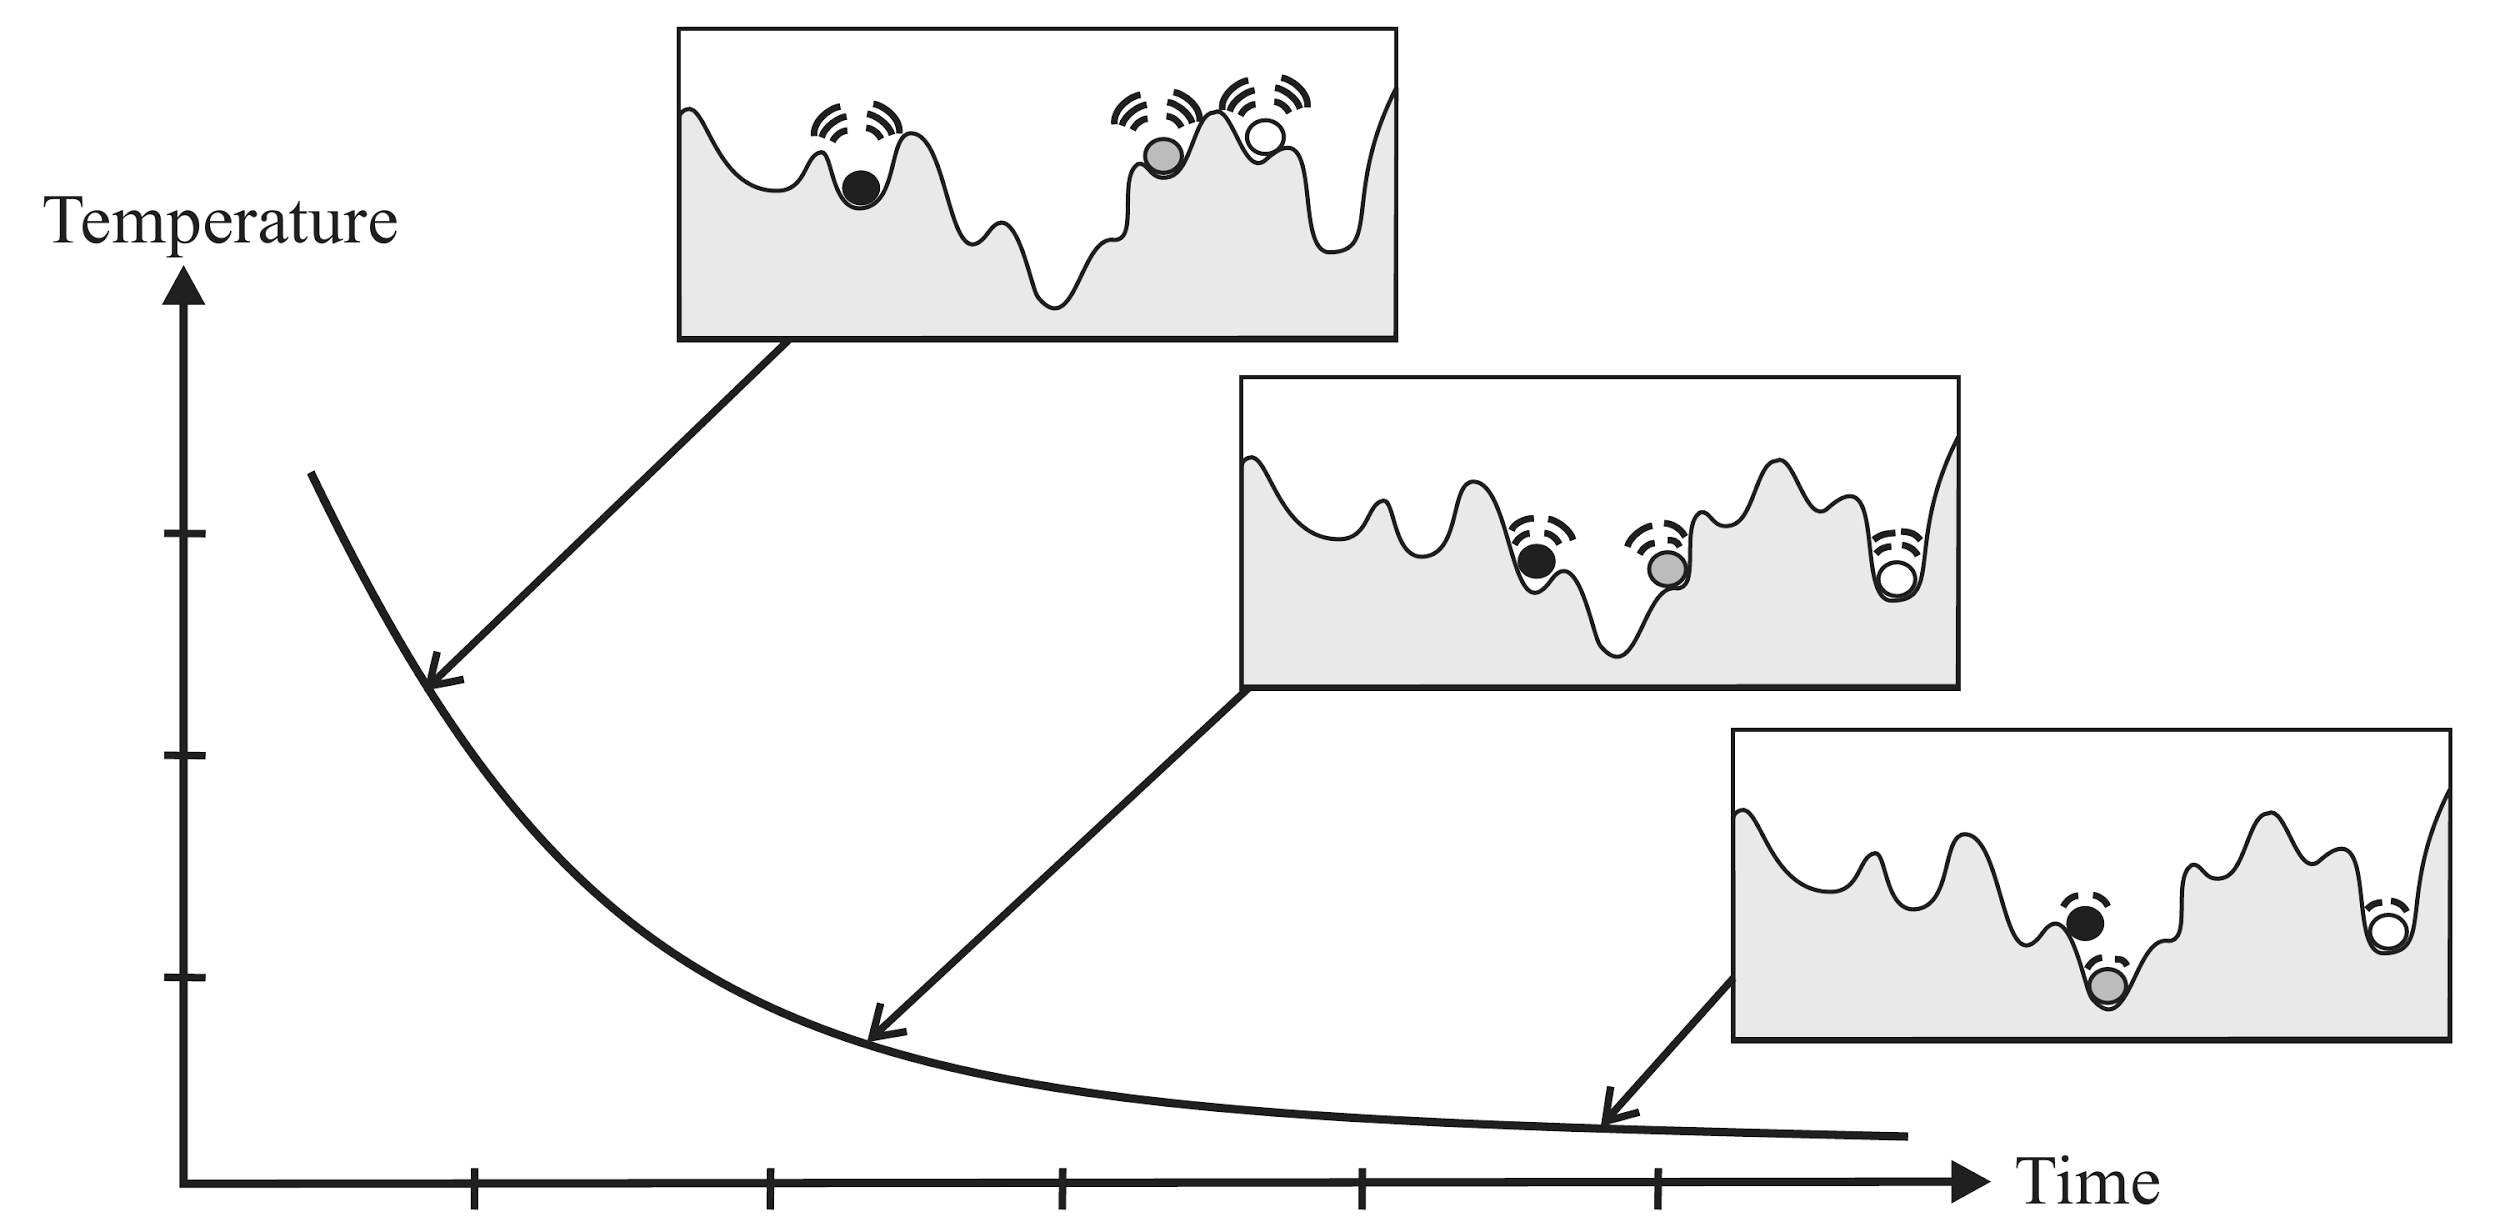
\includegraphics[scale=0.185]{imagens/simulated-annealing.png}
    \end{center}
    \legend{Fonte: \cite{LEDESMA}}
\end{figure}

Problemas no campo das heurísticas podem ser modelados como problemas de
maximização e problemas de minimização de uma função objetivo, que neste
caso é obter a maior cobertura e qualidade do sinal \emph{wireless} na
região informada.

Com um problema de otimização em mãos, encontrar soluções ótimas ou
aproximadas do seu ótimo para problemas NP-difícil é um desafio nem
sempre fácil de ser alcançado. O uso de heurística para auxiliar na
busca por um lugar para o \emph{access point} foi de fácil implementação
e, como a maioria das heurísticas, produz boas soluções dentro de um
tempo viável de acordo com os parâmetros estabelecidos.

Abaixo apresentamos o pseudocódigo da metaheurística com funções
genéricas que foram implementadas neste trabalho:

\begin{algorithm}
    \caption{Simulated Annealing}\label{sa}
    \begin{algorithmic}[1]
        \Procedure{SimulatedAnnealing}{$S_{0}$, $M$, $P$, $L$, $ \alpha $}
        
        \State/* Inicialização das variáveis */
        
        \State $S = S_{0}$
        \State $T_{0} = TempInicial()$
        \State $T = T_{0}$
        \State $j = 1$
        
        \State /* Loop principal */
        \State /* Verifica se foram atendidas as condições de termino do algoritmo */
        \Repeat
        
        \State $i = 1$
        \State $nSucesso = 0$
        
        \State /* Loop Interno */
        \State /* Realização de perturbação em uma iteração */
            \Repeat
                \State $S_{i} = Perturba(S)$
                \State $\Delta_{Fi} = f(S_{i}) - f(S)$
                
                \State /*Teste de aceitação de uma nova solução*/
                \If{$(\Delta_{Fi} \leq 0) \textbf{ or } (exp(-\Delta_{Fi}/T) > Randomiza())$}
                    \State $S = S_{i}$
                    \State $nSucesso = nSucesso + 1$
                \EndIf
            
            \State $i = i + 1$
            \Until{($nSucesso  \geq  L$) \textbf{or} ($i > P$)}
        
           \State $T = \alpha \times T$
           \State /* Atualização do Contador de iterações */
           \State $j = j + 1$
        
        \Until{($nSucesso = 0$) \textbf{or} ($j > M$)}
        
        \State /* Saída do Algoritmo */
        \State \Return{$S$}
        
        \EndProcedure
    \end{algorithmic}
\end{algorithm}

Estes são os identificadores utilizados:

\begin{itemize}
\item
  \(S_{0}\): Configuração Inicial (Entrada);
\item
  \(S_{i}\): Configuração da Iteração \(i\);
\item
  \(S\): Configuração Final;
\item
  \(T_{0}\): Temperatura Inicial;
\item
  \(M\): Número máximo de iterações (Entrada);
\item
  \(P\): Número máximo de Perturbações por iteração (Entrada);
\item
  \(L\): Número máximo de sucessos por iteração (Entrada);
\item
  \(\alpha\): Fator de redução da temperatura (Entrada);
\item
  \(f(S_{i})\): Valor da função objetivo correspondente á configuração
  \(S_{i}\);
\item
  \(nSucesso\): Contador de sucesso em uma iteração;
\item
  \(i\) e \(j\): Variáveis de controle de Loops.
\end{itemize}

Além dos indicadores acima, consideremos as seguintes funções:

\begin{itemize}
\item
  \(Perturba(S)\): Função que realiza uma perturbação na Solução \(S\);
\item
  \(Randomiza()\): Função que gera um número aleatório uniforme no
  intervalo \([0, 1]\);
\item
  \(TempInicial()\): Função que calcula a temperatura inicial.
\end{itemize}

Mais adiante, será descrito como a metaheurística foi adaptada para o
problema de otimização para alocação de \emph{access point} nos
ambientes do IFMG \emph{campus} Formiga. Além disso, também serão
apresentados técnicas e resultados de sua utilização.

\section{Linguagem Python}\label{linguagem-python}

A linguagem que foi utilizada para implementar todo o trabalho foi o
Python. A linguagem Python é uma poderosa linguagem de programação e de
fácil aprendizado. Surgiu no final dos anos 80 e foi criada por Guido
Van Rossum. Na época, Guido trabalhava no Centro de Matemática e Ciência
da Computação de Amsterdã, Holanda, no desenvolvimento de outras
linguagens, quando percebeu que o desenvolvimento de utilitários para o
sistema operacional Amoeba (projeto em que também trabalhava na época)
utilizando a linguagem C estava tomando muito tempo e fazê-los em
\emph{Shell Scrip}t não era viável. Precisava de algo que completasse o
que cada linguagem deixava a desejar. Esses foram o principais motivos
que fizeram com que o desenvolvimento do Python realmente tivesse início
no ano de 1989 e nos primeiros meses de 1990 fosse a linguagem mais
utilizada no departamento de Computação de Amsterdã e hoje por muitos
desenvolvedores de software \cite{SILVA}.

O Python é uma linguagem interpretada. Isso significa que seu código é
executado por um interpretador, e não compilado para linguagem de
máquina para depois ser executada para um sistema e arquitetura
específica, como acontece em algumas linguagens, como por exemplo a
linguagem C \cite{MAGNUN}.

Não obstante, o Python não trabalha com tipagem de objetos, o que
permite, no geral, um ótimo desempenho. Alguns processamentos que
realizam a demanda de mais recursos, como o processamento de imagens,
são feitos por bibliotecas que geralmente são escritas em C ou C++,
inclusive com possíveis trechos em \emph{assembly}, quando o alto
desempenho é necessário. Sendo assim, tais processamentos não fazem uso
de tantos recursos num \emph{script} escrito em Python. Em outra
linguagem compilada seriam exigidos mais recursos.

Mesmo que o Python faça uso bem definido do tipo de dados que está
manipulando, ele trabalha com tipagem dinâmica. Isso implica que uma
variável possuirá características de um tipo específico de sua
declaração, até ser declarada novamente \cite{MAGNUN}. Pode-se ver então
que, com o uso da tipagem dinâmica, são geradas flexibilidade e
simplicidade no código de funções e classes do Python, reduzindo
significativamente a quantidade de parâmetros em uma função.

A separação de blocos no Python não é feita com colchetes, chaves ou
\emph{begins} e \emph{ends}. Toda a separação dos blocos é feita por
tabulações. Isso força sempre o programador a manter o código mais
organizado, além de reduzir consideravelmente o tamanho do código. Caso
o programador que escreveu o código não mantenha a indentação, um erro
de indentação é mostrado e ele não é executado.

Além dos tipos primitivos como \emph{int}, \emph{float} e
\emph{boolean}, também estão presentes no Python tipos especiais como
listas, sendo listas bem definidas entre colchetes e elementos mutáveis
separados por vírgulas; tuplas sendo agora elementos imutáveis definidos
entre parênteses, separados por vírgula e dicionários definidos entre
chaves com tipos imutáveis variados. O conceito de Orientação a Objetos
também está presente no Python, no qual todas as variáveis são definidas
como objeto, até mesmo os tipos primitivos. Todos esses tipos especiais
enriquecem ainda mais o poder que a linguagem tem \cite{GUIDO}. O que em
outra linguagem levaria tempo e linhas de código para ser feito, no
Python é feito com simplicidade.

\section{Bibliotecas utilizadas}\label{bibliotecas-utilizadas}

Uma das vantagens de se usar o Python, é seu vasto número de bibliotecas
embutidas e bibliotecas externas, as quais dão diversas facilidades ao
resolver problemas simples do dia a dia até problemas mais complexos.
Para o desenvolvimento do projeto foram utilizadas várias bibliotecas
que estão embutidas no Python, que vieram complementar outras
bibliotecas externas essenciais para o resultado esperado fosse obtido.

De início, foi utilizada a biblioteca \emph{ezdxf}\footnote{\url{https://pypi.python.org/pypi/ezdxf}}.
Tal biblioteca é um pacote do Python criado para manipular arquivos DXFs
exportados do ** independentemente de sua versão. Com ela, é possível
criar, abrir, salvar e modificar arquivos com a extensão \emph{.dxf} sem
perder qualquer informação, podendo depois, ser utilizada em outros
programas que utilizam a mesma extensão de arquivo. Tal biblioteca está
presente desde o Python 2.7.

Outra biblioteca utilizada no projeto é a PyGame\footnote{\url{https://www.pygame.org/}}.
Seu desenvolvimento teve início no ano 2000 por Pete Shinners, sendo um
código livre e é principalmente usada em aplicações que utilizam
recursos multimídia e/ou programação gráfica, como em desenvolvimento de
jogos multiplataforma (independentemente do sistema operacional).

\section{Programação Paralela}\label{programauxe7uxe3o-paralela}

A computação paralela realizada por placas de vídeo é o uso de uma GPU
juntamente com uma CPU para acelerar aplicações que necessitam de um
alto recurso computacional \cite{KIRK}. Desde 2007, quando a NVIDIA
criou o conceito de `computação acelerada', o uso da GPU vem
potencializando \emph{data centers} de eficiência energética em
laboratórios governamentais, universidades, corporações e empresas de
médio e grande portes em todo o mundo. Elas desempenham um papel
fundamental na aceleração de aplicações em plataformas que variam de
inteligência artificial até carros, drones e robôs \cite{NVIDIA}.

A seguir serão descritos algum conceitos e ferramentas que foram
utilizadas para o desenvolvimento deste trabalho. Todas tiveram um papel
essencial para que os objetivos propostos fossem alcançados.

\subsection{CUDA}\label{cuda}

CUDA\footnote{\url{http://www.nvidia.com.br/object/cuda_home_new_br.html}}
é um acrônimo de \emph{Compute Unified Device Architecture}. É uma
plataforma de computação paralela e um modelo de programação inventados
pela NVIDIA \cite{NVIDIA}. Tal plataforma faz com que as aplicações
tenham aumentos significativos de desempenho computacional ao aproveitar
a potência e os recursos da GPU\footnote{\url{http://www.nvidia.com.br/object/what-is-gpu-computing-br.html}}.
Hoje há milhões de GPUs habilitadas para que trabalhem juntamente com
CUDA. Muitos cientistas e pesquisadores vêm descobrindo inúmeras
possibilidades para o uso da computação com GPU CUDA . Dentre as
possíveis aplicações estão: a identificação de placas ocultas em
artérias em pacientes com problemas de ataque cardíaco, análise do fluxo
de tráfego aéreo junto ao \emph{National Airspace System} (Sistema de
Espaço Aéreo Nacional), aumento de desempenho para a simulação de
visualização de moléculas \cite{KIRK}.

Há algum tempo era complicado escrever códigos para que fossem
executados utilizando a GPU. Todo o assunto sobre programação paralela
em GPU era focado em processamento de imagens; hoje esse conceito já não
é o mesmo. A placa de vídeo faz mais do que realizar o processamento de
imagens; ela lida com um \emph{teraflop} de desempenho de ponto
flutuante e processa tarefas que vão de problemas de finanças à
medicina.

Para que seja possível escrever um código que busque aproveitar o
desempenho oferecido pelo \emph{hardware} juntamente com a CUDA, será
necessário utilizar o CUDA Toolkit, que oferece um ambiente de
desenvolvimento abrangente para desenvolvedores C, C\#, C++, Fortran, R
e Python. O CUDA Toolkit inclui compilador, bibliotecas de matemática e
ferramentas para depuração e otimização do desempenho do código
\cite{FARBER}.

Hoje a NVIDIA oferece todas a ferramentas necessárias para o
desesenvolvimento utiliazando seu \emph{hardware}. Tanto a NVIDIA quando
a CUDA só tendem a crescer, à medida que cada vez mais empresas fornecem
ferramentas, serviços e soluções. Além disso, áreas como a ciência e a
medicina podem crescer ainda mais com suas pesquisas \cite{CUDA}.

\subsection{CUDA Tool Kit}\label{cuda-tool-kit}

O CUDA Toolkit\footnote{\url{https://developer.nvidia.com/cuda-toolkit}}
nada mais é que um kit de ferramenta disponibilizado pela NVIDIA. O kit
fornece um ambiente de desenvolvimento para a criação de aplicações a
serem otimizadas em uma GPU. Com o kit de ferramentas é possível
otimizar e implementar códigos escritos utilizando CUDA em sistemas que
aceitam a paralelização com GPU, \emph{workstations}, centro de dados
empresariais, plataforma baseadas em nuvem e supercomputadores HPC
\cite{TOOLKIT}. No pacote vem incluso bibliotecas otimizadas para GPU,
ferramentas para depuração e otimização, um compilador C/C++ e uma
biblioteca de tempo para ser usada nas aplicações que serão
desenvolvidas.

As bibliotecas otimizadas possibilitam a otimização de vários tipos de
aplicação, como por exemplo, aplicações que realizam cálculos
matemáticos utilizando conceitos de álgebra linear, processamento de
imagem e de vídeo, inteligência artificial e até análise de grafos. O
que torna possível desenvolver aplicações personalizadas para diferentes
linguagens é o uso da API. A API fornece um controle mais seguro e
objetivo, especialmente sobre o contexto ou módulo que a aplicação está
sendo desenvolvida. Uma chamada feita diretamente ao \emph{kernel} é
muito mais complexa de ser implementada, pois a configuração de execução
e os parâmetros do \emph{kernel} devem ser especificados com chamadas de
funções muito bem explícitas. Outra grande vantagem da API é que seu uso
é independente da linguagem.

A versão utilizada neste trabalho foi a CUDA Tool Kit 9.0 e foi o que
tornou possível a otimização do algoritmo na sua versão final. O CUDA
Tool Kit foi instalado juntamente com os \emph{drivers} de vídeo e é
facilmente encontrado no site de desenvolvedores da NVIDIA.

\subsection{Numba}\label{numba}

O Numba\footnote{\url{http://numba.pydata.org/}} é um compilador para
\emph{arrays} e funções numéricas em Python que proporciona a aceleração
de módulos do código, escritos diretamente na linguagem Python. O Numba
realiza a geração de código de máquina otimizado a partir do código
escrito em Python puro, utilizando a infra-estrutura do compilador LLVM
(instalado no momento da instalação do CUDA) \cite{LAM}. Com algumas
anotações simples nos cabeçalhos dos métodos, o código escrito
utilizando vetores e matrizes pode ser otimizado em \emph{just-in-time}
com um desempenho semelhante ao C, C++ e Fortran, sem ter que alterar a
linguagem de programação ou interpretador do Python.

Os principais pontos positivos da utilização do Numba são:

\begin{itemize}
\item
  geração de código \emph{on-the-fly} (geração de código em tempo de
  execução);
\item
  geração de código nativo para a CPU e hardware GPU;
\item
  integração com a pilha de bibliotecas científicas do Python, graças ao
  Numpy.
\end{itemize}

\subsection{\texorpdfstring{JIT
(\emph{just-in-time})}{JIT (just-in-time)}}\label{jit-just-in-time}

O JIT é uma anotação da biblioteca Numba utilizada como \emph{@jit}
acima do nome do método escrito em Python \cite{RIGO}. O código do
método contido abaixo da \emph{flag} será compilado em tempo de
execução, utilizando o conceito \emph{just-in-time}. O JIT possui a
seguinte assinatura: \emph{@jit(signature, nopython, nogil, cache,
forceobj, locals)}. Os parâmetros não são obrigatórios, o que faz com
que o programador deixa a cargo do compilador escolher as melhores
configurações para a compilação. Uma explicação simples dos parâmetros
podem ser vistos abaixo \cite{NUMBA}.

\begin{itemize}
\item
  \textbf{\emph{signature}} é a assinatura do método pelo qual será
  gerado o código de máquina. A assinatura pode ser uma assinatura
  simples, sendo somente o tipo de retorno ou pode ser uma lista de
  assinaturas contendo cada tipo de dados dos parâmetros do método em
  questão. O tipo de retorno pode ser omitido, sendo mostrado apenas o
  tipo dos parâmetros e pode ser utilizado o tipo definido pelo Numba,
  por exemplo: \emph{(numba.int32, numba.double)}. Caso queira deixar
  bem definido o tipo retorno, pode ser usado da seguinte forma:
  \emph{numba.void (numba.int32, numba.double)}. Outra forma de definir
  é usando o nome simples do tipo dos dados, assim: \emph{void(int32,
  double)};
\item
  \textbf{\emph{nopython}} é um valor booleano quando seu valor for
  \emph{true}; força o método a ser compilado no modo
  \emph{``nopython''}. Neste modo de compilação, o Numba gera código que
  não acessa a API Python C. Este modo de compilação produz o código de
  desempenho mais alto, mas requer que os tipos nativos de todos os
  valores no método possam ser inferidos. Caso contrário, o \emph{@jit}
  retornará automaticamente um erro se não puder ser usado;
\item
  \textbf{\emph{forceobj}} é um valor booleano quando seu valor for
  \emph{true}. Força o método a ser compilado no modo objeto. Como o
  modo objeto é mais lento que o modo \emph{nopython}, isso é
  principalmente útil para fins de teste. Esta \emph{flag} faz com que o
  modo de compilação Numba que gera o código que manipula todos os
  valores como objetos Python e usa a API Python C para executar todas
  as operações nesses objetos. O código compilado no modo objeto
  geralmente executará não mais rápido do que o código interpretado pelo
  Python, a menos que o compilador Numba possa aproveitar o mesmo código
  já compilado;
\item
  \textbf{\emph{nogil}} é um valor booleano que, quando seu valor for
  \emph{true}, tenta liberar o bloqueio de interpretação global dentro
  do método compilada. O GIL (\emph{global interpreter lock}) só será
  liberado se o Numba puder compilar a função no modo \emph{nopython},
  caso contrário, um aviso com erro de compilação será exibido;
\item
  \textbf{\emph{cache}}, é um valor booleano que, quando seu valor for
  \emph{true}, habilita um cache baseado em arquivo para encurtar os
  tempos de compilação quando a função já foi compilada em uma invocação
  anterior. O \emph{cache} é mantido no subdiretório
  \emph{\_\_pycache\_\_} do diretório que contém o arquivo de origem.
  Nem todas as funções podem ser armazenadas em cache, uma vez que
  algumas funcionalidades não podem ser sempre persistentes no disco.
  Quando um método não pode ser armazenado em cache, um aviso é emitido
  informando;
\item
  \textbf{\emph{locals}}, é um dicionário que pode ser usado para forçar
  os tipos de dados Numba de variáveis locais particulares, por exemplo,
  se for necessário forçar o uso de variáveis de ponto flutuante com uma
  precisão específica. A documentação do Numba recomenda deixar o
  compilador definir os próprios tipos de variáveis.
\end{itemize}

Para a versão final do algoritmo deste trabalho, foi utilizada a
anotação \emph{@jit}, porém deixado com que o compilador escolhesse
quais dados e forma de compilação usar. O conhecimento e estudo de cada
parâmetro foi essencial para seguir com o desenvolvimento. Caso o
programador decida definir qual a precisão utilizar e otimizar ainda
mais o desempenho do código, é essencial um conhecimento mais
aprofundado do compilador \emph{just-in-time}.

\subsection{Anaconda Navigator}\label{anaconda-navigator}

A Anaconda\footnote{\url{https://www.anaconda.com/}} é uma plataforma
bastante popular de dados científicos para Python e é utilizada por 4.5
milhões de usuários em todo o mundo. Está sempre liderando projetos de
código aberto como Numpy e SciPy, que atualmente formam a base de muitas
aplicações no meio científico \cite{ANACONDA}. A Anaconda também pode
ser utilizada e integrada com a linguagem utilizando o RStudio\footnote{\url{https://www.rstudio.com/}}.

A plataforma pode ser obtida através do site oficial. Após a instalação,
se o usuário achar preferível usar uma interface gráfica, deve-se usar o
Navigator; caso prefira usar o próprio terminal, basta usar o
\emph{conda}. É possível alternar entre eles (qualquer modificação feita
em uma biblioteca será refletida no outro). O Anaconda acaba sendo a
interface gráfica para o \emph{conda}. É possível instalar, remover ou
atualizar qualquer pacote científico da Anaconda com apenas alguns
cliques, utilizando o Navigator ou apenas um único comando do conda no
terminal.

A versão do conda utilizada neste trabalho foi a versão 4.3.30 e a
versão utilizada na interface gráfica, Anaconda Navigator, foi a 1.6.9.

\chapter{PROJETO E DESENVOLVIMENTO}\label{projeto-e-desenvolvimento}

Foram conduzidos estudos bibliográficos para compreensão dos modelos
físicos de propagação de sinais \emph{wireless} em pequena e grande
escala, levando em conta as perdas de sinal e sua atenuação
\cite{ALMERS}. Então foi feito um levantamento do estado da arte sobre
simulação da propagação de sinais, tal como, por exemplo, a modelagem da
propagação de sinais de rádio através de \emph{Ray Tracing}\footnote{\url{https://en.wikipedia.org/wiki/Ray_tracing_(graphics)}}
\cite{YUN}, visando à definição da técnica a ser utilizada para a
simulação da propagação dos sinais \emph{wireless}\\
\cite{LENTZ, NAJNUDEL, SANDEEP}. Uma vez definido o mecanismo de
simulação, foi definida qual técnica de otimização seria aplicada para o
problema da maximização da cobertura de sinal do(s) AP(s) \emph{Wi-Fi},
bem como definida a função objetivo para avaliar as soluções propostas.
Por fim, foi utilizado um método de visualização da intensidade do sinal
\emph{wireless} \cite{RENSBURG,SULAIMAN} , por meio de um mapa de calor
(\emph{heat map}).

\section{Representação do
ambiente}\label{representauxe7uxe3o-do-ambiente}

Os modelos bidimensionais dos ambientes utilizados como caso de estudo
foram o piso 2 do bloco A e os pisos 1, 2 e 3 do bloco C, onde
atualmente os professores e alunos têm reclamado de baixa cobertura de
sinal Wi-Fi. Especificamente, os ambientes da sala dos professores e da
sala de estudos tem apresentado baixa cobertura de sinal Wi-Fi, com
frequentes desconexões dos usuários que ali estejam. Tipicamente, os
pavimentos de edifícios e residências são representados através de
softwares CAD, tais como o AutoCAD\footnote{\url{https://www.autodesk.com.br/products/autocad/overview}}.
Entretanto, softwares CAD tipicamente utilizam um formato proprietário
(DWG no caso do AutoCAD) e como este trabalho se propõe a seguir a
filosofia de software livre e de código-fonte aberto (FOSS\footnote{\url{https://www.gnu.org/philosophy/floss-and-foss.html}}),
optamos por utilizar um formato de entrada interoperável chamado
DXF\footnote{\url{https://www.loc.gov/preservation/digital/formats/fdd/fdd000446.shtml}}
(\emph{Drawing Interchange Format}), que pode ser facilmente exportado a
partir dos \emph{softwares} CAD popularmente utilizados.

\subsection{Arquivo DXF}\label{arquivo-dxf}

O software desenvolvido neste trabalho deve receber como arquivo de
entrada uma representação bidimensional do ambiente a ser simulado,
esperando como tal um arquivo com extensão DXF. Arquivos DXF são comuns
na exportação de desenhos e projetos de peças para serem utilizadas em
softwares de CAM e máquinas de corte automáticas. São populares por
promoverem a troca aberta destes arquivos entre programas desenvolvidos
por diferentes empresas\footnote{Disponível em
  \url{https://www.otimizenesting.com.br/single-post/2016/09/29/Arquivo-DXF}.
  Acesso em 29 out. 2017.}. Para interpretar o arquivo de entrada DXF,
foi implementado um procedimento escrito na linguagem Python utilizando
alguns recursos da biblioteca \emph{ezdxf}, descrita na seção de
materiais. Inicialmente, o procedimento realiza a leitura do arquivo DXF
fornecido.

A partir do conteúdo do DXF, é obtido o \emph{modelspace} no qual é
possível buscar os valores (x,y) extremos do modelo 2D. Isto se faz
necessário para que tais extremos sejam subtraídos no momento da leitura
das paredes do edifício, a fim de evitar desperdício de processamento
com as margens da planta-baixa e para que o desenho do ambiente possa se
enquadrar perfeitamente na tela de visualização do mesmo. Tanto na busca
dos valores limítrofes de x e y, quanto na leitura das linhas do modelo
DXF, é feita uma busca em seu \emph{modelspace} utilizando um laço de
repetição. Na busca, é verificado se o tipo de dados no
\emph{modelspace} é do tipo LINE (linha) e se a camada percorrida é do
tipo ARQ (arquitetura). Durante a verificação de linhas na camada ARQ,
são adicionados a uma lista de paredes as coordenadas do ponto inicial
(x1,x1) e ponto final (x2,y2) de cada linha representada no arquivo DXF,
pois cada linha na camada ARQ do modelo representa uma parede. Observe
que cada coordenada (x,y) deve ser devidamente multiplicada pela escala
definida pelo usuário, para que seja mantido a proporção entre o tamanho
da matriz de simulação e o ambiente real simulado. Ao final do
processamento do arquivo DXF, os valores máximos (e mínimos) das
coordenadas (x,y), bem como cada tupla de coordenadas das paredes é
armazenada em memória pelo \emph{software}, para que sejam utilizados
pela heurística.

\subsection{Escala e precisão}\label{escala-e-precisuxe3o}

Observe que, a partir dos valores (x,y) limítrofes obtém-se as dimensões
do modelo bidimensional e, desde que esteja disponível a informação
sobre o tamanho real do edifício, pode-se calcular a escala da
planta-baixa para o tamanho real do edifício. De posse das dimensões da
planta-baixa e do edifício, pode-se representá-lo computacionalmente
como um arranjo bidimensional, ou seja, uma matriz de tamanho
Comprimento \(X\) Largura, podendo ser utilizada uma escala 1:1 do
ambiente simulado para o ambiente real. Neste caso, uma célula da matriz
representaria 1 \(m^{2}\) no mundo real.

Entretanto, vale ressaltar que o \emph{software} produzido é capaz de
trabalhar com diferentes níveis de precisão na simulação de propagação
de sinais, onde caso o usuário queira uma precisão de 0,5 \(m^{2}\) por
célula da matriz, bastaria informar tal configuração de forma que o
\emph{software} passe a utilizar um fator de escala de 2.0x a dimensão
real do edifício (pois precisão = 1/escala). Assim, o software pode
trabalhar com a precisão desejada pelo usuário, podendo inclusive
realizar uma simulação de propagação de ondas onde cada célula da matriz
tenha a dimensão de um comprimento de onda \((\lambda = c/f)\). Por
exemplo, se o usuário desejar ter a precisão de 1 comprimento de onda
para simular a propagação de Wi-Fi na frequência de 2,484 GHz, cada
célula representará\footnote{\(2.998\times10^{8} m/s \div 2.437\) GHz
  \url{https://www.wolframalpha.com/input/?i=c+\%2F+2.437+GHz}} uma área
de 12,3 \(cm^{2}\). Entretanto, vale ressaltar que quanto maior a
precisão da simulação, maior serão as dimensões da matriz que representa
o ambiente e, portanto, mais demorada será a simulação computacional.

As plantas-baixas representando os ambientes simuladores neste trabalho
foram gentilmente cedidas pela equipe de TI do campus Formiga (bloco A)
e com o setor de engenharia civil do campus Formiga (no caso dos blocos
B e C). A \autoref{repre_ambiente_dxf_1} ilustra o ambiente do bloco A
do campus Formiga, tendo sido carregado automaticamente a partir do
arquivo DXF. O texto descrevendo no que consiste cada sala do ambiente
foi adicionado posteriormente à captura da imagem, para melhor
compreensão e localização do leitor.

\begin{figure}[htb]
    \caption{\label{repre_ambiente_dxf_1} Representação do ambiente a partir do arquivo DXF contendo a planta-baixa}
    \begin{center}
        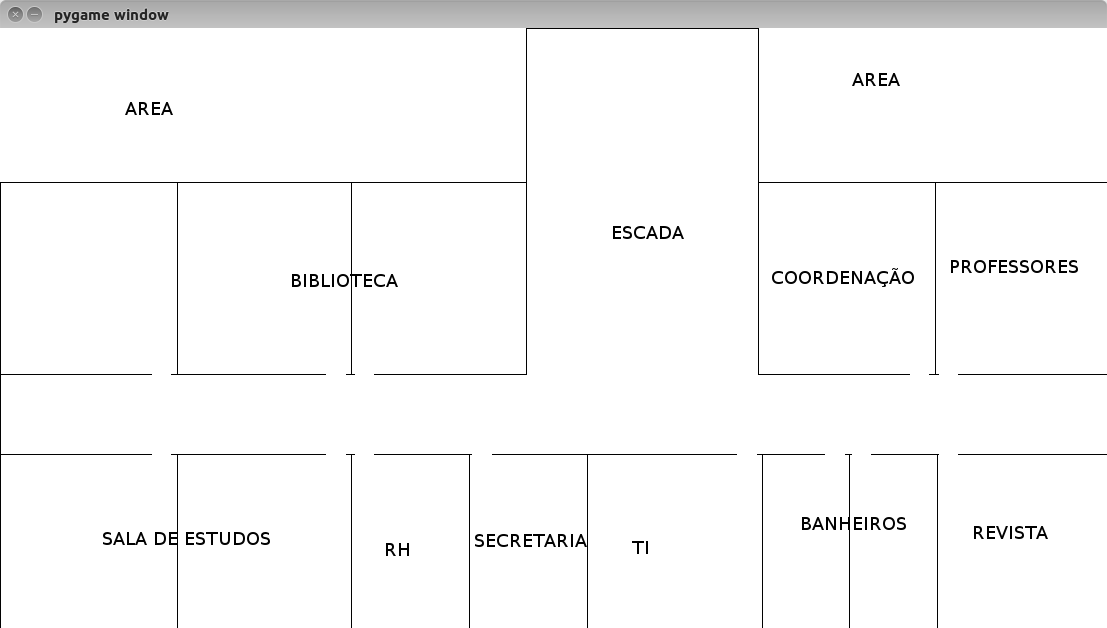
\includegraphics[scale=0.4]{imagens/planta-labels.jpg}
    \end{center}
    \legend{Fonte: Elaborado pelo autor}
\end{figure}

Para a visualização dos resultados dos testes e uma melhor interpretação
dos resultados, foi utilizado o PyGame para prover a visualização
gráfica da matriz contendo os resultados dos cálculos de intensidade de
sinal em cada ponto do modelo simulado, conforme proposto pelo modelo de
propagação utilizado. Após a representação da matriz de propagação no
PyGame, podem ser desenhadas também as paredes do ambiente simulado de
acordo com a lista de linhas obtidas no processamento do arquivo DXF. A
maneira como a representação visual do ambiente simulado foi realizada
será tratada em detalhes em seção posterior.

\section{Propagação dos sinais}\label{propagauxe7uxe3o-dos-sinais}

Conforme assunto abordado na seção onde foram falados sobre os modelos
de propagação, se faz necessário uma boa escolha de qual modelo de
propagação de sinais utilizar, para obter uma boa representação da
intensidade dos sinais para aquela banda do espectro eletromagnético e,
assim, simular algo mais próximo da realidade. Quanto maior for a
precisão desejada para o valor da intensidade de sinal devido a perdas e
sua atenuação, mais detalhes sobre o ambiente de propagação devem ser
modelados (frequências, distâncias, paredes, pisos, materiais, etc).

\subsection{Definição do modelo de propagação para sinais
Wi-Fi}\label{definiuxe7uxe3o-do-modelo-de-propagauxe7uxe3o-para-sinais-wi-fi}

Foram conduzidos nas dependências do campus Formiga experimentos para
medição do decaimento da intensidade do sinal \emph{Wi-Fi}. Foram
realizadas medições \emph{indoor} nos corredores do campus. Para tal,
foi posicionado no corredor um \emph{access point} Cisco WAP200 (IEEE
802.11b/g) e configurado para utilizar um canal \emph{Wi-Fi} que
correspondesse a uma frequência que, naquele momento, estivesse livre de
interferência de outros APs naquela região do campus. A potência máxima
de transmissão que o AP suporta é -14 \(dBm\) (0,0398 mW), mas ele foi
configurado para utilizar apenas \(25\%\) dessa potência. Tal
configuração visou apenas reduzir a distância a ser percorrida na
condução do teste, uma vez que as paredes e pisos absorvem mais ou menos
o sinal de acordo com a frequência dele e não de sua intensidade,
portanto manteve-se o comportamento esperado na propagação do sinal. O
\emph{access point WAP200} utilizado como transmissor possui antenas com
2 \(dBi\) de ganho e a interface Wi-Fi do notebook utilizado como
receptor nos testes possui ganho de 1 \(dBi\). Foi utilizado o canal 11
(portanto com frequência de 2,462 GHz e \(\lambda\) de 12,18 cm), tendo
sido realizadas medições após o campo distante da antena (campo de
\emph{Fraunhofer} = 148 cm).

As medições foram coletadas utilizando o comando \emph{iwlist} da
biblioteca \emph{iw-utils}, que realiza a varredura (\emph{scanning}) da
faixa de espectro correspondente ao Wi-Fi e registra os valores de
intensidade de sinal recebidos bem como o endereço MAC do(s) AP(s). A
\autoref{medicao_modelos} ilustra quão bem cada modelo de propagação
considerado previu o valor da intensidade de sinal de acordo com com o
aumento da distância. Pela figura, observe que o modelo de reflexão de
dois raios, por definição e de acordo com a altura das antenas
(aproximadamente 90 cm, considerando também o suporte utilizado), seria
apropriado somente se as distâncias entre transmissor e receptor fossem
superiores a 83,59 m, faixa demasiado próxima do limite de alcance de um
enlace \emph{Wi-Fi} típico. Também, observe que com o modelo de
propagação no espaço livre (modelo de \emph{Friis}), as estimativas
foram abaixo do valor real observado, por tal modelo não considerar os
fenômenos de reflexão, difração e dispersão que tipicamente ocorrem na
propagação de ondas em um ambiente geometricamente complexo (paredes,
piso, teto, portas, janelas, mobília, etc).

\begin{figure}[htb]
    \caption{\label{medicao_modelos} Medição da intensidade de sinal $vs.$ modelos de sua propagação}
    \begin{center}
        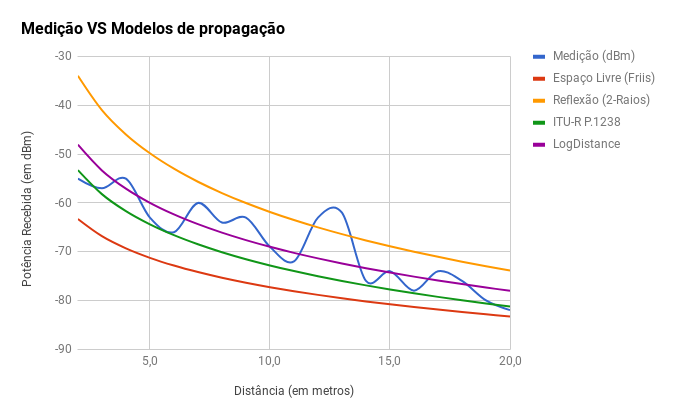
\includegraphics[scale=0.68]{imagens/medicao-modelos.jpg}
    \end{center}
    \legend{Fonte: Elaborado pelo autor}
\end{figure}

Pela é possível observar que, dos modelos de propagação analisados, o
\emph{LogDistance Path Loss} apresentou um bom casamento entre os
valores de suas estimativas e os valores reais mensurados, sendo
portanto considerado como o mais promissor. Entretanto, observe que a
\autoref{medicao_modelos} apresenta apenas uma das várias medições
realizadas, ilustrando portanto o decaimento exponencial da intensidade
do sinal \emph{Wi-Fi} ao longo de um corredor do bloco B. Neste caso, o
modelo \emph{LogDistance} foi calibrado para uma distância de referência
(\(d_{0}\)) de 10 metros com a respectiva perda (\(PL_{0}\)) mensurada
em -69 \(dBm\), com expoente de perda de caminho manualmente ajustado
como \(\gamma\) = 3 (\emph{path loss exponent}).

\subsection{Ajuste do modelo de
propagação}\label{ajuste-do-modelo-de-propagauxe7uxe3o}

Não podemos basear nossa simulação em parâmetros de um modelo de
configuração calibrado para medições coletadas em \emph{apenas um
corredor de um pavimento de um prédio do campus Formiga}. Se faz
necessário calibrar o modelo de propagação para que que seja mais
abrangente para o \emph{campus}, devendo ser calibrado de acordo com
múltiplas medições realizadas em diversas salas, corredores e áreas
internas de nosso caso de estudo.

Para tal, as informações de distância \emph{vs.} intensidade das várias
medições conduzidas foram utilizadas como entrada para um ajuste de
curvas estatístico, técnica de regressão que foi conduzida no
\emph{software} \emph{R-Project}\footnote{\url{https://www.r-project.org/}}.
Inicialmente, conduzimos regressões com um ajuste de curvas estatístico
utilizando os pacotes \emph{fitdistrplus}\footnote{\url{https://cran.r-project.org/web/packages/fitdistrplus/index.html}}
e \emph{FAdist}\footnote{\url{https://cran.r-project.org/web/packages/FAdist/index.html}}
do software \emph{R-Project}.

\begin{figure}[htb]
    \caption{\label{curvas} Ajuste de curvas da 2P-Logística, 3P-LogNormal e 3P-LogLogística}
    \begin{center}
        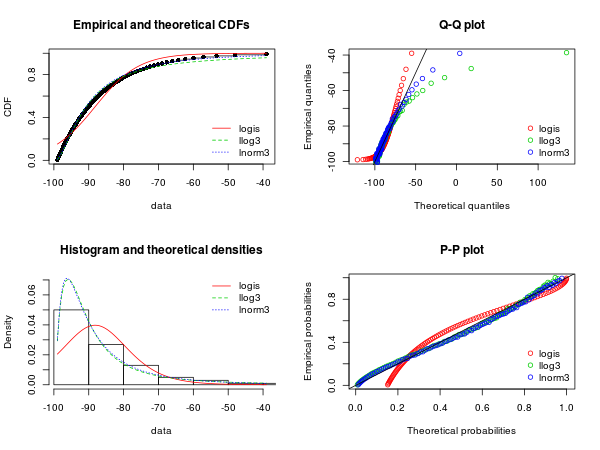
\includegraphics[scale=0.8]{imagens/curvas.jpg}
    \end{center}
    \legend{Fonte: Elaborado pelo autor}
\end{figure}

Pela comparação do ajuste de curvas ilustrado na \autoref{curvas},
observamos que a distribuição Logística com apenas 2 parâmetros (logis)
não consegue modelar bem o decaimento do nível de sinal observado na
medições do RSSI no campus Formiga. Por outro lado, as distribuições
3P-LogNormal (lnorm3) e 3P-LogLogistica (llog3) se aproximaram bem do
comportamento esperado para o decaimento da intensidade do sinal,
estando tal fato em consonância com o exposto nas seções
\ref{sec:log_normal_fading} (\emph{Log-normal fading}) e
\ref{sec:log_distance} (\emph{Log-distance}).

A \autoref{log_logistica} e a \autoref{log_normal} apresentam em
detalhes a qualidade do ajuste de curvas estatístico, obtido através das
regressões realizadas. Ao comparar o GOF (\emph{Goodness-of-fit}) entre
duas ou mais distribuições, pode-se considerar os critérios de qualidade
do ajuste AIC (\emph{Akaike's Information Criterion}) e BIC
(\emph{Bayesian Information Criterion}).

\begin{figure}[htb]
    \caption{\label{log_logistica} Qualidade do ajuste (GOF) da distribuição 3P-LogLogística}
    \begin{center}
        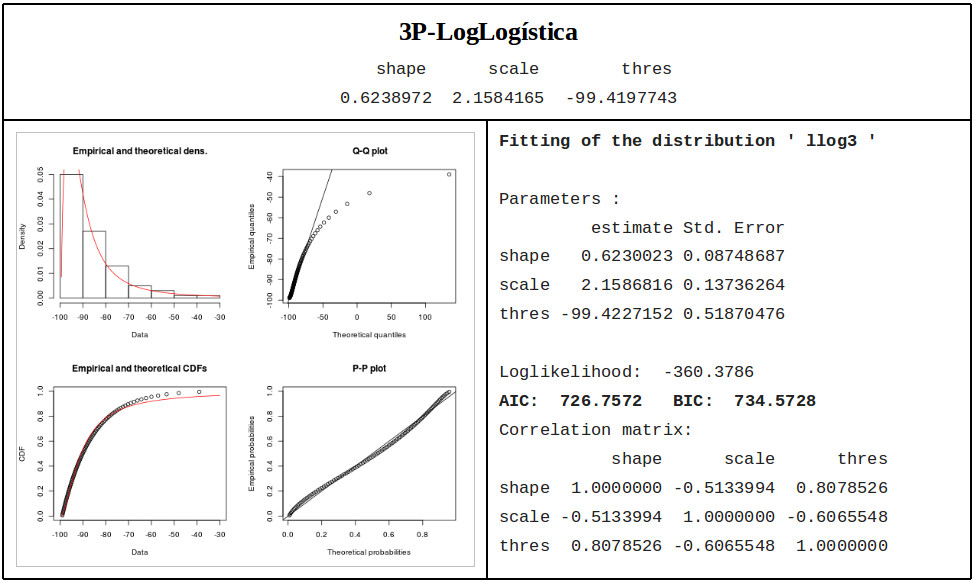
\includegraphics[scale=0.47]{imagens/log-logistica.jpg}
    \end{center}
    \legend{Fonte: Elaborado pelo autor}
\end{figure}
\begin{figure}[htb]
    \caption{\label{log_normal} Qualidade do ajuste (GOF) da distribuição 3P-LogNormal}
    \begin{center}
        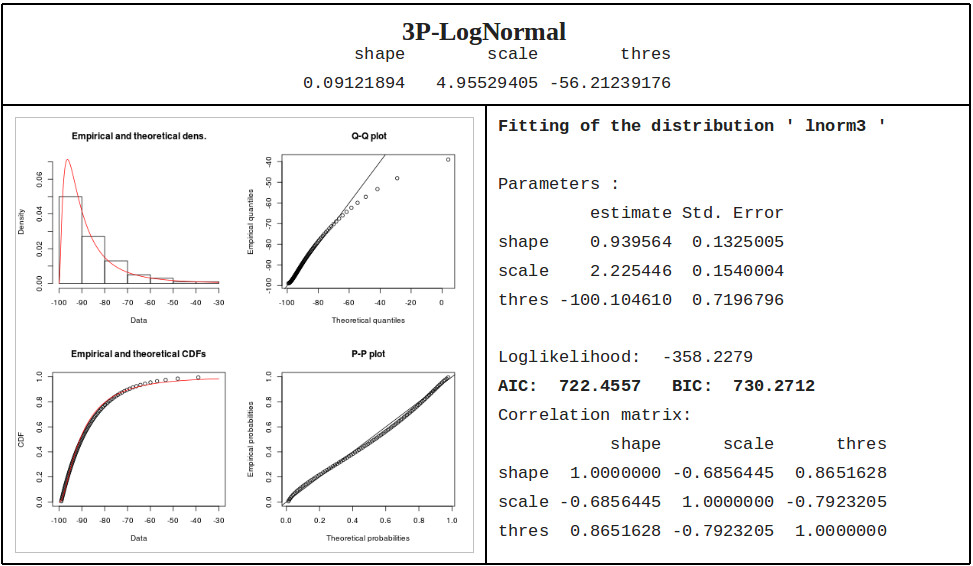
\includegraphics[scale=0.47]{imagens/log-normal.jpg}
    \end{center}
    \legend{Fonte: Elaborado pelo autor}
\end{figure}

Considerando o melhor ajuste das distribuições LogNormal e LogLogistica,
ambas com 3 parâmetros, passamos a considerar uma regressão estatística
com distribuições estatísticas mais complexas, de 4 ou mais parâmetros,
mas mantendo o comportamento logarítmico. Uma regressão
\textbf{NP-Logística} foi conduzida com a utilização do pacote
\emph{nplr}, também no software \emph{R-Project}.

Para obtermos um melhor resultado, considerando o bom desempenho das
distribuições LogNormal e LogLogística, instruímos o modelo de regressão
Logístico a utilizar uma base logarítmica para os valores do eixo \(x\),
ou seja, a distância ao AP deve ser interpretada como \(log_{10}(x)\).
Em uma livre interpretação, isso corresponderia a instruir a regressão
logística a utilizar modelos NP-LogLogísticos. Assim, buscamos partir
dos bons resultados obtidos na análise prévia, mas tentando melhorá-los
com a inclusão de um quarto ou quinto parâmetros de ajuste da
distribuição. Obtivemos um melhor \emph{fitness} com um modelo Logístico
de 4 parâmetros (\emph{4-Parameter Logistic} ou simplesmente 4PL),
conforme resultados apresentados a seguir. Conforme ilustra a e a , o
melhor ajuste de curva (GOF) foi obtido com uma distribuição
4P-Logística e com a distância fornecida em em escala logarítmica, como
\(log_{10}(x)\) metros.

\begin{figure}[htb]
    \caption{\label{logistic_regression_1} Previsão de RSSI da 4P-LogLogística para distâncias em $ log_{10}(x) $ metros}
    \begin{center}
        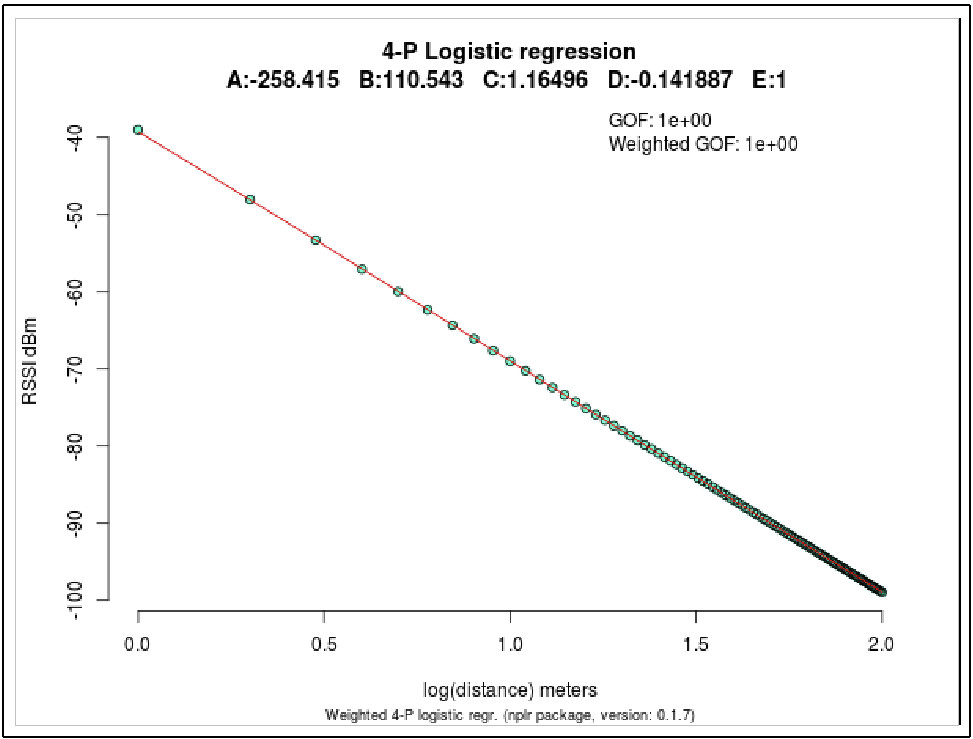
\includegraphics[scale=0.47]{imagens/logistic-regression-1.jpg}
    \end{center}
    \legend{Fonte: Elaborado pelo autor}
\end{figure}
\begin{figure}[htb]
    \caption{\label{logistic_regression_2} Previsão de RSSI da 4P-Logística para distâncias em metros}
    \begin{center}
        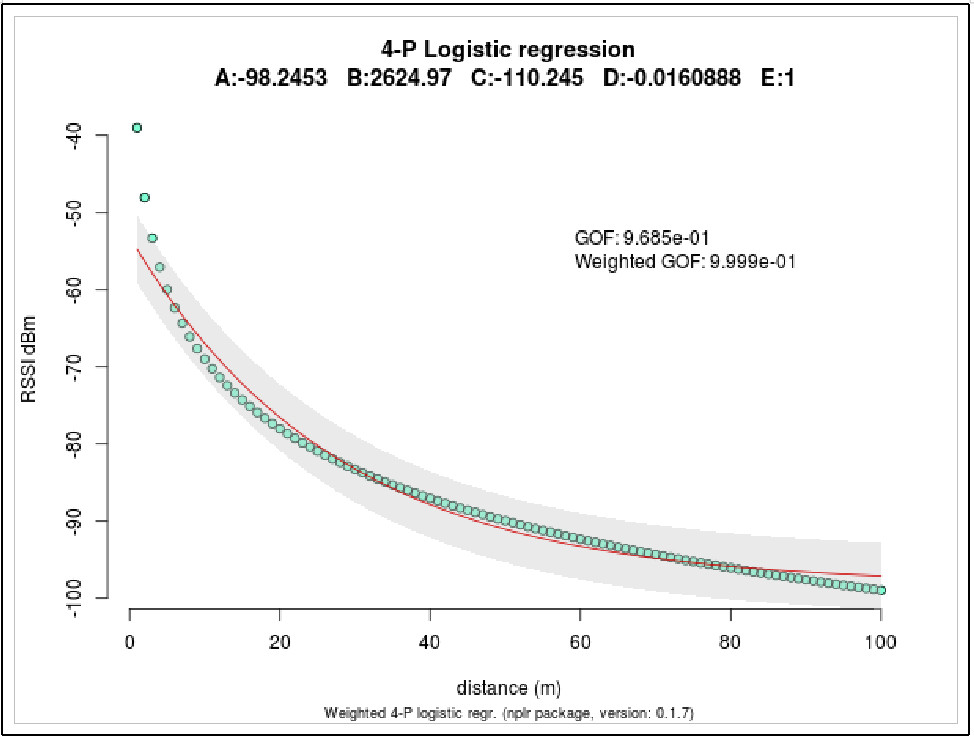
\includegraphics[scale=0.47]{imagens/logistic-regression-2.jpg}
    \end{center}
    \legend{Fonte: Elaborado pelo autor}
\end{figure}

Enfim, a partir dos parâmetros da 4P-Logística (4PL ou logis4) obtidos
pela regressão, podemos configurar as constantes de sua equação e, a
partir dela, obtiver a estimativa de decaimento do nível de sinal com o
aumento da distância do AP, calibradas para a realidade do campus
Formiga. A equação característica de uma NP-Logística de cinco
parâmetros é:

\begin{equation}
f(x; A,B,C,D,E) = D + (A-D) / ( (1+(x/C)^B)^E )
\end{equation}

na qual os parâmetros A, B, C, D e E são obtidos ao aplicar-se a
regressão logística para os valores de intensidade de sinal (em \(dBm\)
ou mW). Observe que, fixando ``\(E=1\)'' obtemos a equação da \(4PL\)
(\emph{4-Parameter Logistic}) e se fixarmos ambos ``\(D=0\)'' e
``\(E=1\)'', obtemos a equação da 3PL (\emph{3-Parameter Logistic}). Os
cinco parâmetros da \(NP-Log\) tem o seguinte significado:

\begin{itemize}
\item
  A = Mínima assintótica. Em medições da propagação de sinais de rádio,
  considere-o como o valor do sinal para uma distância de referência. Em
  propagação de sinais de rádio, tipicamente é o valor do sinal a 10
  metros do transmissor. No caso do \emph{Wi-Fi}, será um valor de
  referência aferido após o campo distante da antena (distância de
  \emph{Fraunhoffer}), ou seja, intensidade do sinal aferida a 2 metros
  (2,4 GHz) ou 4 metros (5,6 GHz);
\item
  B = Inclinação da curva, que pode ser positiva ou negativa. No caso de
  propagação de sinais de rádio, para obtermos um decaimento do sinal
  provavelmente B será positivo;
\item
  C = Ponto de inflexão, definido como o ponto onde a curvatura muda de
  direção ou sinal. \(C\) é a concentração onde \(y = \frac{(D-A)}{2}\).
  No caso do Wi-Fi, provavelmente será o valor do sinal aferido em torno
  10 a 20 metros;
\item
  D = Máxima assintótica. Em medições da propagação de sinais de rádio,
  considere-o como o valor do sinal para uma distância muito grande. No
  caso do \emph{Wi-Fi}, pode-se utilizar um valor de referência aferido
  a 100 metros (limita da WLAN);
\item
  E = Fator de assimetria. Para E=1, temos uma curva simétrica em torno
  do ponto de inflexão e, portanto, temos uma equação logística de
  quatro parâmetros.
\end{itemize}

Para utilizar tal distribuição estatística como modelo de propagação,
deve-se implementar no \emph{software} sua \textbf{função de densidade
de probabilidade} (PDF) para que possa retornar qual seria o valor da
intensidade do sinal recebido (RSSI) em determinada distância do AP
\emph{Wi-Fi}. Durante a implementação, vale observar que ambas as
distribuições \emph{4P-Log} e LogDistance devem ser utilizadas como um
modelo de \textbf{perda de sinal}, ou seja, o valor da estimativa obtido
(\(PL\)) deve ser subtraído da potência de transmissão (\(P_{t}\)) do AP
para obter a previsão da potência recebida (\(P_{r}\)):

\begin{equation}
Pr(x) = Pt - PL(x)
\end{equation}

onde \(P_{r}\) é a potência recebida à distância \(x\) do transmissor;
\(P_{t}\) é a potência do sinal do transmissor (ex.: -20 \(dBm\)) e
\(PL\) é a perda do sinal ao longo do caminho entre o transmissor e
receptor (calculada com a equação da 4PL ou da \emph{LogDistance}).
Inicialmente, implementamos tais fórmulas em uma planilha para
visualizarmos graficamente uma comparação das medições de RSSI
realizadas no campus com a expectativa de decaimento proporcionado pelos
modelos LogDistance e 4P-Logístico. A \autoref{modelos_propagacao}
ilustra o decaimento se sinal previsto por cada um dos modelos acima
citados em relação aos valores reais de medição coletados.

\begin{figure}[htb]
    \caption{\label{modelos_propagacao} Comparação dos modelos de propagação LogDistance e NP-Logístico}
    \begin{center}
        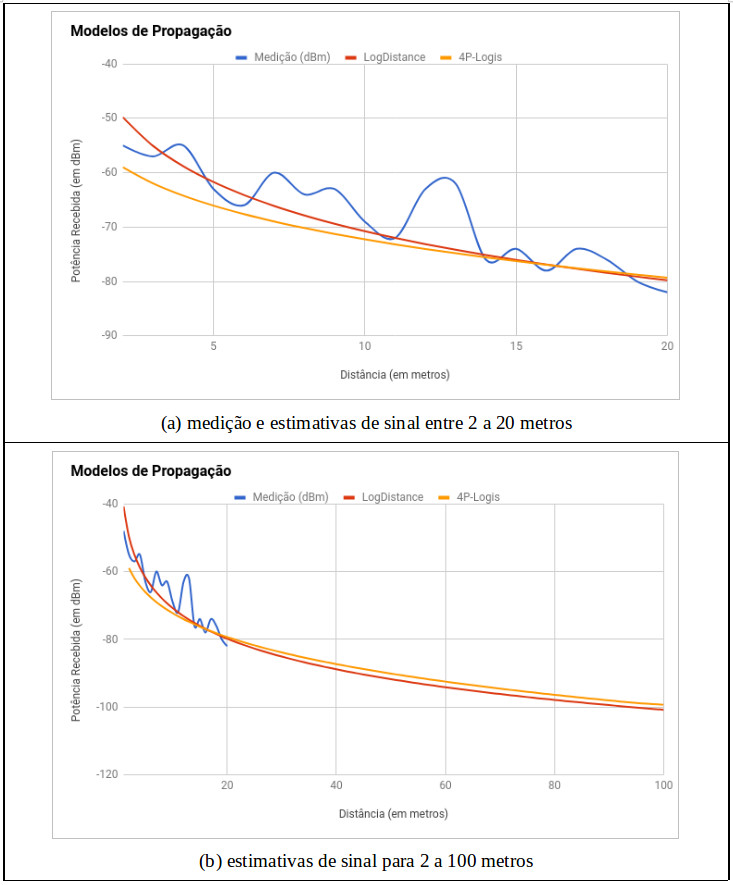
\includegraphics[scale=0.6]{imagens/modelos-propagacao.jpg}
    \end{center}
    \legend{Fonte: Elaborado pelo autor}
\end{figure}

Já na \autoref{modelos_propagacao} (b), é apresentada a extrapolação que
os modelos de propagação de fornecem para distâncias de até 100 metros
(limite de alcance de um sinal \emph{Wi-Fi} \emph{indoor}. Comparando as
\autoref{modelos_propagacao} (a) e (b), é interessante notar que os dois
modelos diferiram mais para curtas distâncias, escala onde acontece
muita variação do nível de sinal devido aos efeitos de múltiplas
reflexões nas paredes, difração nas portas, dispersão e absorção pelos
materiais. Isto está plenamente de acordo com a abordagem do assunto
pela literatura, no que tange a modelos de propagação de pequena e larga
escala \cite{RAPPAPORT}.

\subsection{Simulação da propagação de sinais no
ambiente}\label{simulauxe7uxe3o-da-propagauxe7uxe3o-de-sinais-no-ambiente}

Como dito anteriormente, para a realização dos cálculos, o ambiente foi
representado como uma matriz bidimensional, representando em escala o
ambiente a ser simulado. Cada posição {[}x,y{]} da matriz é um ponto
candidato a hospedar o \emph{access point} (AP). Uma vez determinada a
proposta de nova localização do AP, para cada posição da matriz é
necessário realizar o cálculo do modelo de propagação. Na configuração
do \emph{software} produzido, pode-se informar a posição atual do AP no
ambiente real, ou deixar que o \emph{software} inicie a exploração a
partir de uma posição aleatória. Para preencher os valores da matriz
representando a propagação do sinal de microondas, deve-se realizar o
cálculo determinado pelo modelo de propagação, conforme tratado na seção
anterior. Tipicamente, como os modelos de propagação fazem uso da
distância entre o transmissor e receptor, esta deve ser calculada
utilizando as coordenadas do \emph{access point} na simulação e do ponto
para o qual deseja-se calcular a estimativa da intensidade do sinal alí
recebido (RSSI).

A \autoref{wifi_central} exibe uma representação gráfica da matriz com
os valores de intensidade de sinal conforme o decaimento exponencial da
intensidade do sinal recebido (RSSI), com o aumento da distância de cada
ponto da matriz com o AP \emph{Wi-Fi} (ponto central).

\begin{figure}[htb]
    \caption{\label{wifi_central} Decaimento RSSI de $Wi-Fi$ de acordo com a distância ao AP}
    \begin{center}
        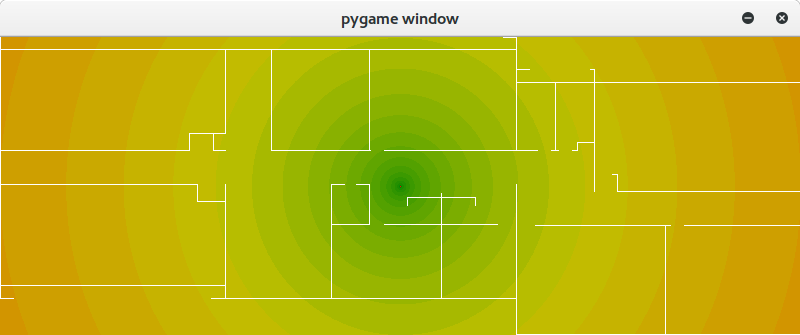
\includegraphics[scale=0.5]{imagens/wifi-central.jpg}
    \end{center}
    \legend{Fonte: Elaborado pelo autor}
\end{figure}

Neste ponto, vale notar que o escopo deste trabalho não considera
interferências entre canais \emph{Wi-Fi} de vários APs, de maneira que
para cada AP simulado é gerada uma matriz numérica individual, que
receberá as estimativas de valores para a intensidade de sinal em
decibel \emph{miliWatt} (\(dBm\)). O propósito deste trabalho é sugerir
um melhor posicionamento dos APs e a decisão de não terem sido modeladas
interferências entre APs diferentes é baseada no fato de que a
tecnologia \emph{Wi-Fi} possibilita coexistência de alguns APs em um
mesmo ambiente, desde que o canal central de cada AP esteja
suficientemente espaçado dos demais. Por exemplo, nos padrões IEEE
802.11b/g/n a largura de banda é de 20 MHz e portanto podem coexistir
até quatro APs em um mesmo ambiente, conforme ilustra a
\autoref{canais}.

\begin{figure}[htb]
    \caption{\label{canais} Canais não sobrepostos para WLANs de 2,4 GHz}
    \begin{center}
        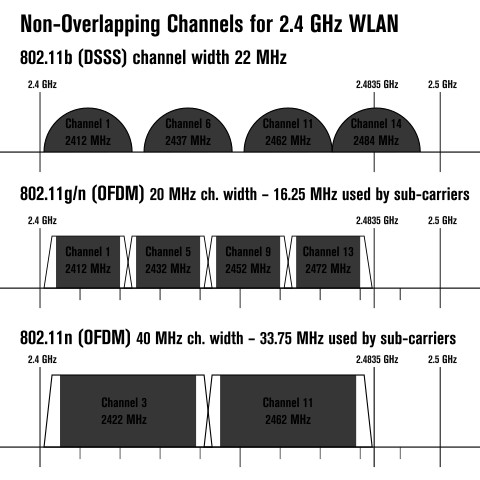
\includegraphics[scale=0.6]{images/canais-1.jpg}
    \end{center}
    \legend{Fonte: \url{https://en.wikipedia.org/wiki/File:NonOverlappingChannels2.4GHzWLAN-en.svg}}
\end{figure}

\subsection{Atenuação do sinal ao atravessar
paredes}\label{atenuauxe7uxe3o-do-sinal-ao-atravessar-paredes}

Para obtermos um resultado que fosse condizente com a realidade, ou
seja, que representasse quanto o sinal \emph{Wi-Fi} degradava à medida
que se propagava através de cômodos em sequência, foi adicionada uma
técnica para realizar estimativas da absorção do sinal ao atravessar
paredes. Na planta-baixa do edifício, todas as linhas (que representam
paredes e divisórias) são armazenadas em uma estrutura de dados no
início do programa, antes de iniciar a simulação. Tais linhas se
mostraram úteis para simular de maneira mais próxima da realidade o
valor da intensidade do sinal em um determinado ponto, atravessando o
ambiente simulado desde o AP até tal ponto.

Seguimos a modelagem utilizada pela literatura para modelos de
propagação em pequena escala, onde o valor esperado para o sinal em
determinado ponto é subtraído do valor em \(dB\) que representa a
energia absorvida por parede multiplicado pela quantidade de paredes
atravessadas pelo sinal. A literatura sugere que o valor de absorção
varia entre 8 e 15 \(dB\) para paredes de concreto \cite{RAPPAPORT}, de
maneira que o valor definido para para uso do \emph{software} produzido
na simulação do campus Formiga foi de 8 \(dB\) (e de acordo com análise
experimental). Vale observar que, por consistir em uma constante que
pode ser configurada no \emph{software}, a ordem de magnitude da
absorção de energia pelas paredes do edifício pode ser ajustada para que
a simulação da propagação possa se aproximar da realidade daquele
ambiente.

Para ilustrar o resultado de aplicar tal fator de correção, observe na
\autoref{absorcao_parede} a mesma simulação da figura anterior, porém
agora contabilizando a absorção do sinal \emph{Wi-Fi} a cada parede
atravessada no trajeto do AP ao ponto destino.

\begin{figure}[ht]
    \caption{\label{absorcao_parede} Absorção do sinal por cada parede atravessada.}
    \begin{center}
        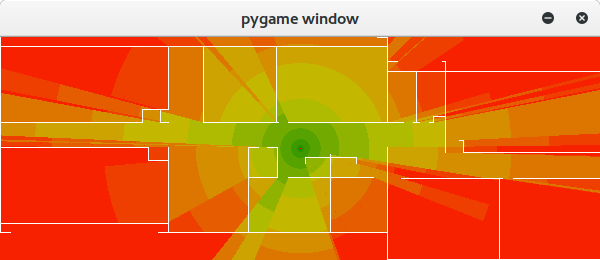
\includegraphics[scale=0.7]{imagens/absorcao-parede.jpg}
    \end{center}
    \legend{Fonte: Elaborado pelo autor}
\end{figure}

Para ter uma noção de quantas paredes o sinal sofreria atenuação, foram
utilizadas equações de geometria euclidiana. No momento em que se faz
necessário o cálculo da absorção das paredes para um ponto {[}x, y{]}
qualquer da matriz, a lista de linhas representando as paredes da
planta-baixa deve ser percorrida. A técnica utilizada foi a intersecção
de retas num plano cartesiano (\emph{Line-Line Intersection}), buscando
definir se os dois segmentos de reta ambas possuem um ponto em comum
(ponto de interseção). A definição de intersecção de retas é dada por
retas concorrentes, ou seja, se possuírem um ponto em comum, então a
intersecção das duas retas será este o ponto em comum. Assim,
viabiliza-se verificar o cruzamento do sinal com paredes a um baixo
custo computacional, se comparado a testar por força bruta cada ponto
interno ao retângulo formado pela parede.

Os segmentos de reta candidatos consistem nas linhas previamente obtidas
do arquivo DXF, contendo a planta-baixa. Cada linha no DXF possui duas
coordenadas bidimensionais, para o ponto inicial e o ponto final do
segmento de reta. O outro segmento de reta é formado entre o AP e o
ponto para o qual está sendo calculada a intensidade do sinal. A
\autoref{intersecao_retas}, ilustra o segmento de reta formado entre um
dado ponto (x1,y1) na matriz e o local do AP (x2,y2), cruzando com um
outro segmento de reta formado pelas extremidades da parede (x3,y3) e
(x4,y4). Caso haja ponto de interseção (x,y) significa que o sinal terá
atravessado tal parede e soma-se um à quantidade de paredes
atravessadas. Caso contrário, se não houver ponto de interseção entre os
dois segmentos de reta, significa que o sinal cruzou livremente o espaço
entre o AP e o destino sem cruzar com tal parede.

\begin{figure}[ht]
    \caption{\label{intersecao_retas} Interseção de retas.}
    \begin{center}
        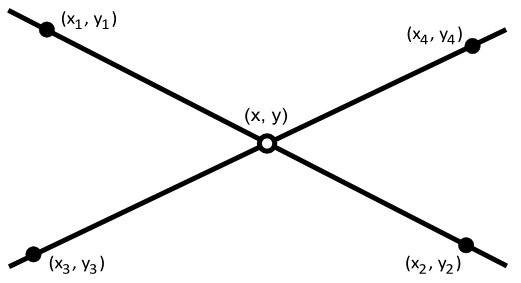
\includegraphics[scale=0.5]{imagens/inter.jpg}
    \end{center}
    \legend{Fonte: Elaborado pelo autor}
\end{figure}

Entretanto, apesar de tal verificação ser barata para um ponto e as
paredes candidatas, deve-se lembrar que é um cálculo a mais a ser
efetuado para cada um dos \(N \times M\) pontos da matriz para cada uma
das \(K\) paredes, ou seja, \(N \times M \times K\) cálculos a serem
efetuados e, portanto, com custo de tempo da ordem de \(O(n^{3})\). E
como o algoritmo de otimização irá avaliar centenas de posicionamentos
para o AP, à medida que explora o espaço de soluções, o custo
computacional sobre para \(N \times M \times K \times P\), ou seja, como
todas estas quantidades possuem uma mesma ordem de magnitude (centenas),
o algoritmo passa a ter custo temporal de \(O(n^{4})\). Assim, com a
adição dessa nova modelagem na propagação do sinal \emph{Wi-Fi}, o tempo
de execução do algoritmo extrapolou os costumeiros segundos e beirou as
dezenas de minutos.

\section{Visualização dos dados}\label{visualizauxe7uxe3o-dos-dados}

A princípio, foi implementada a etapa que trata a representação do
ambiente, ao utilizar a matriz de propagação para a geração do modelo 2D
correspondente à planta-baixa fornecida \cite{KASE,THAKUR}. Tal modelo
pode representar algumas características físicas do ambiente, tais como
paredes e portas \cite{MARSCHALLINGER}, no qual o sinal pode atenuar em
um maior ou menor grau sua intensidade de propagação. A
\autoref{repre_ambiente_dxf_2} ilustra uma representação gráfica das
características da planta baixa do bloco A\footnote{A modelagem de
  ambiente utilizada para as simulações apresenta as mesmas divisões de
  cômodos do arquivo AutoCAD disponibilizado para o este trabalho.},
onde pode-se observar a presença de portas e paredes. Foi registrado o
uso que cada cômodo possui atualmente no campus Formiga.

\begin{figure}[ht]
    \caption{\label{repre_ambiente_dxf_2} Representação do ambiente a partir do arquivo DXF contendo a planta-baixa}
    \begin{center}
        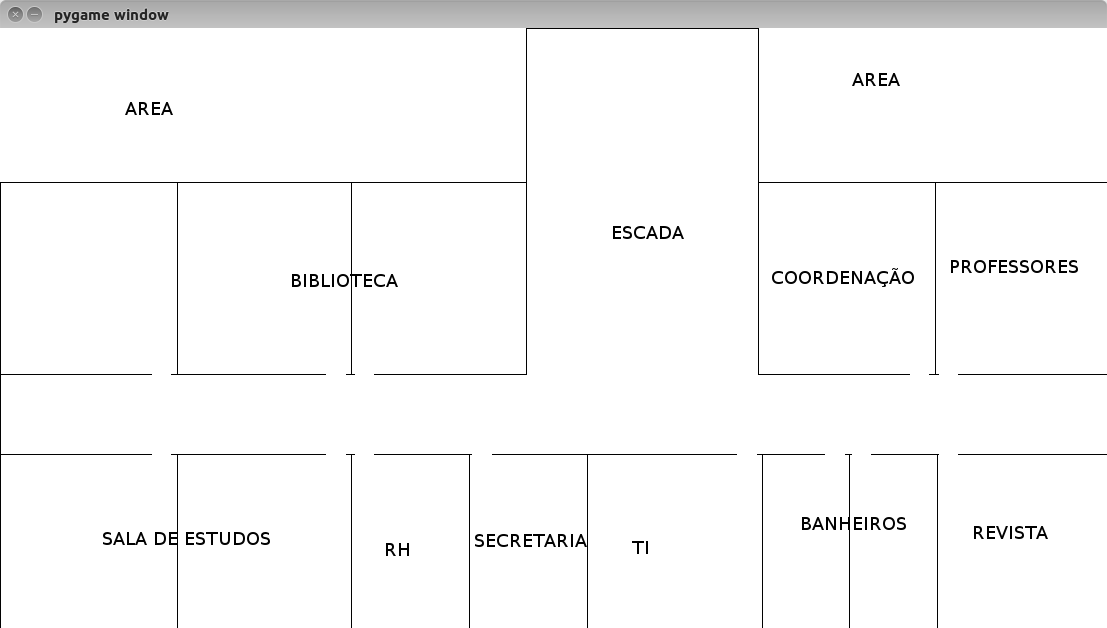
\includegraphics[scale=0.4]{imagens/planta-labels.jpg}
    \end{center}
    \legend{Fonte: Elaborado pelo autor}
\end{figure}

Com o preenchimento da matriz de propagação de acordo com a posição do
\emph{access point} (AP) e com o respectivo valor da intensidade do
sinal, se tornou difícil a visualização de quanto o sinal ficava ruim
quanto maior era a distância e mais paredes eram atravessadas, através
de uma simples inspeção numérica. Tendo a matriz preenchida com a
intensidade de sinal (\(dB\)), suficiente para a realização dos cálculos
com a função objetivo da heurística de otimização, fica pendente a
visualização a olho nú, não sendo viável distinguir dentre milhares de
valores numa matriz, se poderia ser considerada uma simulação boa ou
ruim.

Considerando a vasta quantidade de ferramentas e bibliotecas
disponibilizadas pela linguagem Python, foi necessário utilizar algum
método para transformar a matriz de intensidade de sinais em algo um
tanto quanto visível e de fácil interpretação. Diante disso, o PyGame
foi utilizado na visualização da matriz resultante. Com a obtenção dos
valores máximos e mínimos dentro da matriz de propagação, é fácil
definir uma faixa de valores para calibrar uma escala de referência
(gradiente de cores) para a exposição dos resultados. Para padronizar e
viabilizar a comparação visual de resultados diferentes, o gradiente de
cores foi normalizado para um valor mínimo de referência de -100 \(dB\),
referente à maior sensibilidade registrada pelos equipamentos de
comunicação \emph{Wi-Fi}. Esta visualização dos resultados pode ser
vista na \autoref{represetacao_simulacao}.

\begin{figure}[ht]
    \caption{\label{represetacao_simulacao} Simulação da propagação utilizando 256 cores}
    \begin{center}
        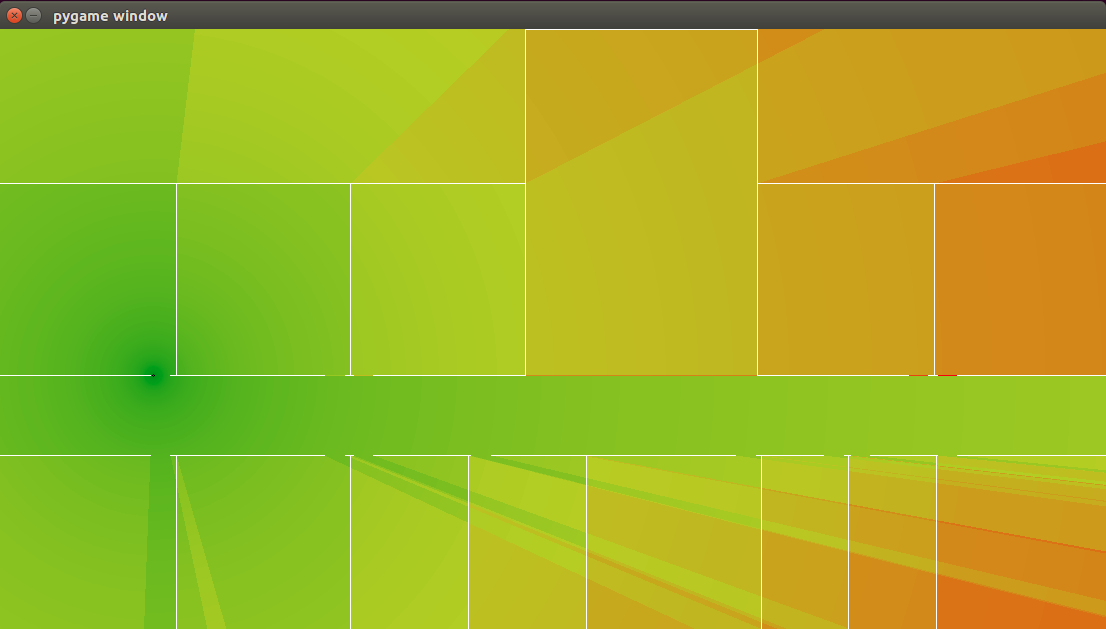
\includegraphics[scale=0.4]{imagens/representacao-simulacao.jpg}
    \end{center}
    \legend{Fonte: Elaborado pelo autor}
\end{figure}

Foi implementado um método capaz de explorar os recursos
disponibilizados pelo PyGame para ilustrar a matriz resultante. Tal
método, que pode ser visto abaixo, percorre a matriz obtendo o valor
calculado em dBm da posição {[}x, y{]} e mapeia uma cor de acordo com o
gradiente de cores escolhido. Adicionalmente, foi utilizada condição que
avalia o valor do sinal em determinado ponto com uma constante que
representa a sensibilidade máxima definida pelos equipamentos de
\emph{Wi-Fi}. Os valores de sensibilidade dos diversos equipamentos
presentes no campus Formiga do IFMG variam entre -85 e -100 \(dB\).
Assim, se o valor calculado para a simulação da propagação for menor que
a sensibilidade do AP, na visualização do mesmo ele é considerado como
um ``ponto cego'' ou uma ``região de sombra'', uma vez que não há
intensidade de sinal suficiente para obter uma boa qualidade de serviço
(ou sequer conectar na rede \emph{Wi-Fi}). A
\autoref{simulacao_sensibilidade} ilustra as regiões de sombra no
ambiente simulado com apenas um AP centralizado transmitindo com uma
potência de -17 \(dB\).

\begin{figure}[ht]
    \caption{\label{simulacao_sensibilidade} Regiões com sinal abaixo da sensibilidade máxima dos equipamentos}
    \begin{center}
        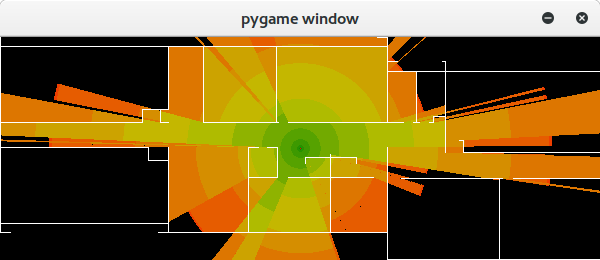
\includegraphics[scale=0.7]{imagens/sumulacao-sensibilidade.jpg}
    \end{center}
    \legend{Fonte: Elaborado pelo autor}
\end{figure}

O algoritmo foi desenvolvido de tal forma que seja possível durante a
exploração do espaço de soluções pelo \emph{Simulated Annealing}, exibir
a matriz de intensidade de sinal a cada iteração para acompanhar o
funcionamento do algoritmo, comportando-se como uma animação em tempo
real. Entretanto, como o desenho dos milhares de pontos pelo PyGame
consiste em uma operação que consome alguns segundos, tal processo de
animação fica desativado por padrão para não retardar o cômputo da
solução final que o usuário aguarda.

\section{Heurística de
otimização}\label{heuruxedstica-de-otimizauxe7uxe3o}

Para o cumprimento dos objetivos e um bom resultado, foi implementada a
metaheurística, que irá explorar o espaço de soluções de posicionamento
dos APs no modelo espacial do ambiente, visando à maximização da
cobertura do sinal (dentre outras possíveis métricas). Conforme exposto
na seção de materiais e métodos, foi utilizada a metaheurística proposta
por Scoot Kirkpatrick \cite{PATRICK}. O \emph{Simulated Annealing} foi
utilizado para a realização do processo de otimização, buscando
encontrar a melhor solução viável, considerando o objetivo do problema
em questão e o conjunto de restrições para aceitação da solução
proposta.

\subsection{\texorpdfstring{Implementação do \emph{Simulated
Annealing}}{Implementação do Simulated Annealing}}\label{implementauxe7uxe3o-do-simulated-annealing}

Inicialmente a metaheurística buscava o melhor ponto apenas para um AP.
Com o cumprimento dos objetivos tornou-se possível a busca e otimização
de mais de um AP. O SA inicia com os valores predefinidos no momento da
sua chamada. Para o método é informado: o número de APs a serem
utilizados no ambiente, o número máximo de iterações, o número máximo de
perturbações por cada iteração, o número máximo de sucessos por iteração
e o \(\alpha\) como o fator de redução da temperatura. Na seção
\ref{sec:avalia_dois_ou_mais} podem ser vistos mais detalhes sobre como
a função objetivo foi implementada.

Com a estratégia de perturbar mais de um AP por vez, o SA inicia
alocando todos os APs na posição central da planta baixa. A primeira
solução é avaliada (APs no centro) para que então seja realizada a busca
e novas perturbações sejam feitas. O SA fica em um \emph{loop}
principal, no qual se verifica se foram atendidas todas as condições de
término do algoritmo (se extrapolou o máximo de iterações ou se nenhum
ponto com ótimo local foi encontrado). Outro \emph{loop} interno realiza
a perturbação dos APs em forma de lista circular. Com os valores de
\(f(S_{i})\) (resultado da avaliação da função objetivo na
\emph{i-ésima} iteração do SA) e \(f(S)\) (melhor resultado da avaliação
da função objetivo iteração do SA) é possível determinar o valor de
\(\Delta F_{i}\) (diferença da avaliação da função objetiva atual com a
avaliação da função objetiva ótima encontrada até o momento). Caso o
valor de \(\Delta F_{i}\) seja menor ou igual a zero, há uma redução de
energia, a qual implica que a nova solução é melhor que a anterior.
Então é aceito a solução e \(f(S_{i})\) passa a ser a nova solução
corrente. A aceitação desse tipo de solução é mais provável em altas
temperaturas e bastante improvável em temperaturas reduzidas. Para
reproduzir essas características, geralmente usa-se, para calcular a
probabilidade de se aceitar a nova solução, uma função conhecida por
critério de aceitação de \emph{Boltzmann} \cite{AARTS}, que em sua
fórmula o valor de \(T\) é a temperatura atual e que regula a
probabilidade de soluções com pior custo. Tal fórmula pode ser vista
abaixo:

\begin{equation}
    e^{(-\Delta/T)}
\end{equation}

Com a aceitação, é atualizada a lista das melhores posições para a
alocação dos APs e também a variável \(f(S)\) com o valor de melhor
função objetivo, o número de sucessos representando a vizinhança, que
também é fator de parada do SA, e o número de perturbações por iteração
é incrementado. O método é finalizado quando a temperatura chega a um
valor próximo de zero, situação esta em que a chance de se aceitar uma
solução vizinha pior é extremamente baixa, ou seja, quando o sistema
estiver estável.

Por fim, a melhor solução encontrada pela metaheurística é retornada,
indicando a proposta do novo posicionamento dos APs e a cobertura do
sinal \emph{Wi-Fi} alcançada, caso tal solução fosse implantada no
ambiente real. Além disso, é fornecida uma visualização gráfica do
resultado a ser obtido com a solução proposta utilizando o PyGame.

\subsection{Calibração dos parâmetros do Simulated
Annealing}\label{calibrauxe7uxe3o-dos-paruxe2metros-do-simulated-annealing}

Definir quais os parâmetros utilizar na metaheurística não é uma tarefa
fácil, então para isso, qualquer ferramenta que auxiliasse neste
processo seria útil. Para a escolha de quais parâmetros utilizar para os
valores foi empregado um Projeto Fatorial \(2^{k}\) com foco no ajuste
do \emph{Simulated Annealing}.

Com a aplicação do planejamento de experimentos é possível definir uma
sequência de coletas de dados experimentais a fim de atingir um
objetivo. Dentre os métodos de planejamento experimental disponíveis na
literatura, o planejamento fatorial é o mais indicado quando se deseja
estudar os efeitos de duas ou mais variáveis de influência, sendo que em
cada tentativa ou réplica, todas as combinações possíveis dos níveis de
cada variável são investigadas \cite{NETO}. O caso mais simples de
planejamento fatorial descrito na literatura é aquele em que cada fator
\(k\) está presente em apenas dois níveis (o experimento aplicado neste
trabalho), ou seja, em um experimento com \(k\) fatores (ou variáveis) e
dois níveis, obtendo-se \(2^{k}\) experimentos a realizar.

Os valores dos parâmetros do SA foram definidos quando ainda estava
sendo utilizado apenas um AP. Para o teste, foram considerados os
valores da quantidade de vizinhos, temperatura inicial, o fator de
resfriamento e a quantidade máxima de perturbações. O valor do máximo de
iterações foi definidos em 50 e a posição do AP foi definida como sendo
{[}0, 0{]}. Foi desenvolvido um \emph{script} em Python que
automatizasse o processo. Como são quatro parâmetros que se deseja saber
os valores e são utilizados dois níveis de profundidade, foi utilizado o
conceito de tabela verdade, contendo \(2^{4}\) linhas fazendo com que
todas as possibilidades de parâmetros sejam testadas.

Com a coleta das informações obtidas pela saída do \emph{script} em
Python, os valores foram adicionados em uma planilha do Excel cedida
pelo orientador. A tabela realiza todos os cálculos necessários para
saber qual parâmetro é mais propício a se utilizar. A
\autoref{tabela_parametros_1} apresenta a configuração da primeira
iteração do planejamento \(2^{k}\) com os fatores e níveis bem
definidos.

\begin{table}[ht]
    \centering
    \caption{Fatores para parâmetro para o \textit{Simulated Annealing} na primeira iteração}
    \label{tabela_parametros_1}
    \resizebox{\textwidth}{!}{%
        \begin{tabular}{|l|l|c|c|c|c|c|c|c|c|c|}
            \hline
            \multicolumn{1}{|c|}{} &  & \multicolumn{4}{c|}{\textbf{FATORES}} & \multicolumn{4}{c|}{\textbf{FATORES}} & \multicolumn{1}{l|}{\textbf{FIXO}} \\ \hline
            \textbf{k=} & 4 & \multicolumn{2}{c|}{\begin{tabular}[c]{@{}c@{}}A\\ (n de vizinhos)\end{tabular}} & \multicolumn{2}{c|}{\begin{tabular}[c]{@{}c@{}}B\\ (temperatura inicial)\end{tabular}} & \multicolumn{2}{c|}{\begin{tabular}[c]{@{}c@{}}C\\ (fator resfriamento)\end{tabular}} & \multicolumn{2}{c|}{\begin{tabular}[c]{@{}c@{}}D\\ (perturbações)\end{tabular}} & Iteracoes \\ \hline
            \multirow{2}{*}{\textbf{n=}} & \multirow{2}{*}{Niveis} & 1 & 20 & 1 & 100 & 1 & 75\% & 1 & 10 & 1000 \\ \cline{3-11} 
            &  & 2 & 40 & 2 & 200 & 2 & 95\% & 2 & 20 & 1000 \\ \hline
        \end{tabular}%
    }
\end{table}

O resultado computado é dado na \autoref{candidatos_parametros_1}:

\begin{table}[ht]
    \centering
    \caption{Candidatos a parâmetros na primeira iteração}
    \label{candidatos_parametros_1}
    \resizebox{\textwidth}{!}{%
        \begin{tabular}{|l|c|c|c|c|}
            \hline
            & \multicolumn{4}{l|}{\textbf{CANDIDATOS A PARÂMETRO}} \\ \hline
            Frações & vizinhos & temperatura & resfriamento & pertubações \\ \hline
            Função Objetivo & 1,4\% & 1,0\% & 1,2\% & 1,0\% \\ \hline
            Tempo & 0,9\% & 0,8\% & 1,2\% & 1,0\% \\ \hline
            MÉDIA & 1,2\% & 0,9\% & 1,2\% & 1,0\% \\ \hline
        \end{tabular}%
    }
\end{table}

Com o resultado acima, é possível notar que o melhor candidato é o
número de vizinhos e o resfriamento. O valor dado em porcentagem
representa o quanto promissor é ao ser tomado como um valor de parametro
para o \emph{Simulated Annealing}. Ainda que o valor de ambos tenha sido
o mesmo, o número de vizinhos acaba sendo melhor, pois consumiu uma
fração menor do tempo total. O número de vizinhos foi aumentado para ter
um resultado melhor ainda; os valores da temperatura inicial também
foram aumentados e o fator de resfriamento foi decrementado junto com o
número de perturbações. Modificando os parâmetros, se torna propício a
um novo melhor conjunto de valores do SA. Os novos valores da segunda
iteração do planejamento fatorial \(2^{k}\) podem ser vistos na
\autoref{tabela_parametros_2}.

\begin{table}[ht]
    \centering
    \caption{Fatores para parâmetro para o \textit{Simulated Annealing} na segunda iteração}
    \label{tabela_parametros_2}
    \resizebox{\textwidth}{!}{%
        \begin{tabular}{|l|l|c|c|c|c|c|c|c|c|c|}
            \hline
            \multicolumn{1}{|c|}{} &  & \multicolumn{4}{c|}{\textbf{FATORES}} & \multicolumn{4}{c|}{\textbf{FATORES}} & \multicolumn{1}{l|}{\textbf{FIXO}} \\ \hline
            \textbf{k=} & 4 & \multicolumn{2}{c|}{\begin{tabular}[c]{@{}c@{}}A\\ (n de vizinhos)\end{tabular}} & \multicolumn{2}{c|}{\begin{tabular}[c]{@{}c@{}}B\\ (temperatura inicial)\end{tabular}} & \multicolumn{2}{c|}{\begin{tabular}[c]{@{}c@{}}C\\ (fator resfriamento)\end{tabular}} & \multicolumn{2}{c|}{\begin{tabular}[c]{@{}c@{}}D\\ (perturbações)\end{tabular}} & Iterações \\ \hline
            \multirow{2}{*}{\textbf{n=}} & \multirow{2}{*}{Niveis} & 1 & 40 & 1 & 150 & 1 & 75\% & 1 & 10 & 1000 \\ \cline{3-11} 
            &  & 2 & 80 & 2 & 300 & 2 & 85\% & 2 & 15 & 1000 \\ \hline
        \end{tabular}%
    }
\end{table}

O resultado dado pela configuração da \autoref{tabela_parametros_2} pode
ser visto na \autoref{candidatos_parametros_2}:

\begin{table}[ht]
    \centering
    \caption{Candidatos a parâmetros na segunda iteração}
    \label{candidatos_parametros_2}
    \resizebox{\textwidth}{!}{%
        \begin{tabular}{|l|c|c|c|c|}
            \hline
            & \multicolumn{4}{l|}{\textbf{CANDIDATOS A PARÂMETRO}} \\ \hline
            Frações & vizinhos & temperatura & resfriamento & pertubações \\ \hline
            \textbf{Função Objetivo} & 1,4\% & 1,0\% & 1,3\% & 1,0\% \\ \hline
            \textbf{Tempo} & 1,2\% & 0,9\% & 1,2\% & 1,1\% \\ \hline
            \textbf{MÉDIA} & 1,3\% & 0,9\% & 1,2\% & 1,0\% \\ \hline
        \end{tabular}%
    }
\end{table}

Como na iteração anterior, o melhor candidato a manter o seu valor é o
número de vizinhos. Com a análise feita, o número de vizinhos no segundo
nível e a temperatura inicial também obtiveram um bom resultado no
segundo nível. O valor do resfriamento no segundo nível manteve sua
média, enquanto o número de perturbações em ambos os níveis, teve um
resultado inferior ao anterior, sendo necessário modificá-lo na próxima
iteração. Na \autoref{tabela_parametros_3} é possível ver como ficaram
definidos os parâmetros para a terceira iteração e último teste.

\begin{table}[ht]
    \centering
    \caption{Fatores para parâmetro para o \textit{Simulated Annealing} na terceira iteração}
    \label{tabela_parametros_3}
    \resizebox{\textwidth}{!}{%
        \begin{tabular}{|l|l|c|c|c|c|c|c|c|c|c|}
            \hline
            \multicolumn{1}{|c|}{} &  & \multicolumn{4}{c|}{\textbf{FATORES}} & \multicolumn{4}{c|}{\textbf{FATORES}} & \multicolumn{1}{l|}{\textbf{FIXO}} \\ \hline
            \textbf{k=} & 4 & \multicolumn{2}{c|}{\begin{tabular}[c]{@{}c@{}}A\\ (n de vizinhos)\end{tabular}} & \multicolumn{2}{c|}{\begin{tabular}[c]{@{}c@{}}B\\ (temperatura inicial)\end{tabular}} & \multicolumn{2}{c|}{\begin{tabular}[c]{@{}c@{}}C\\ (fator resfriamento)\end{tabular}} & \multicolumn{2}{c|}{\begin{tabular}[c]{@{}c@{}}D\\ (perturbações)\end{tabular}} & Iteracoes \\ \hline
            \multirow{2}{*}{\textbf{n=}} & \multirow{2}{*}{Niveis} & 1 & 80 & 1 & 300 & 1 & 80\% & 1 & 5 & 1000 \\ \cline{3-11} 
            &  & 2 & 60 & 2 & 600 & 2 & 85\% & 2 & 10 & 1000 \\ \hline
        \end{tabular}%
    }
\end{table}

De acordo com a configuração da \autoref{tabela_parametros_3} são dados
os candidatos a parâmetros expostos na
\autoref{candidatos_parametros_3}.

\begin{table}[ht]
    \centering
    \caption{Candidatos a parâmetros na terceira iteração}
    \label{candidatos_parametros_3}
    \resizebox{\textwidth}{!}{%
        \begin{tabular}{|l|c|c|c|c|}
            \hline
            & \multicolumn{4}{l|}{\textbf{CANDIDATOS A PARÂMETRO}} \\ \hline
            Frações & vizinhos & temperatura & resfriamento & pertubações \\ \hline
            \textbf{Função Objetivo} & 1,4\% & 1,0\% & 1,3\% & 1,0\% \\ \hline
            \textbf{Tempo} & 1,2\% & 0,9\% & 1,1\% & 1,1\% \\ \hline
            \textbf{MÉDIA} & 1,3\% & 0,9\% & 1,2\% & 1,0\% \\ \hline
        \end{tabular}%
    }
\end{table}

Os resultados apresentados acima passaram por três refinamentos. Assim,
como dito no início desta seção, o teste foi realizado com o intuito de
aprimorar os parâmetros do \emph{Simulated Annealing} com apenas um AP.
A estratégia para a versão final e com múltiplos \emph{access points} é
definir também como um fator (variável), o valor do raio de perturbação
e fazer com que ele seja uma porcentagem da largura da matriz de
propagação, tornando-o dinâmico de acordo com o tamanho da planta. A
\autoref{parametros_metaheuristica} mostra de uma forma melhor como
ficaram os parâmetros utilizados na metaheurística:

\begin{table}[]
    \centering
    \caption{Parâmetros definitivos utilizados na metaheurística}
    \label{parametros_metaheuristica}
    \resizebox{\textwidth}{!}{%
        \begin{tabular}{|c|c|c|c|c|c|}
            \hline
            \textbf{\begin{tabular}[c]{@{}c@{}}Raio de \\ perturbação\end{tabular}}              & \textbf{\begin{tabular}[c]{@{}c@{}}Número máximo\\  de iterações\end{tabular}} & \textbf{\begin{tabular}[c]{@{}c@{}}Número máximo \\ de perturbações\end{tabular}} & \textbf{\begin{tabular}[c]{@{}c@{}}Número máximo \\ de vizinhos\end{tabular}} & \textbf{\begin{tabular}[c]{@{}c@{}}Decaimento da \\ temperatura (Alpha)\end{tabular}} & \textbf{\begin{tabular}[c]{@{}c@{}}Temperatura \\ inicial\end{tabular}} \\ \hline
            \begin{tabular}[c]{@{}c@{}}WIDTH * 0.025\\ (2.5\% da largura da matriz)\end{tabular} & 600 *  APs                                                                & 5                                                                                 & 80                                                                            & 85\%                                                                                  & 300 *  APs                                                            \\ \hline
        \end{tabular}%
    }
\end{table}

A resolução foi dada em metros e transformada de uma forma compatível
com o processamento e a duração esperada para analisar cada solução. Os
parâmetros definidos para a alocação de vários APs foi um compilado dos
parâmetros utilizados no \emph{Simulated Annealing} com um AP juntamente
com testes feitos repetidas vezes.

\section{Avaliação da solução}\label{avaliauxe7uxe3o-da-soluuxe7uxe3o}

Nesta seção apresentaremos como foram implementadas as técnicas
utilizadas para avaliações com um ou mais \emph{access points} bem como
o aperfeiçoamento da função objetivo.

\subsection{Avaliação da solução com um AP}\label{sec:avalia_one_ap}

Para a implementação do SA, se faz importante a decisão de uma boa
função objetivo. A função objetivo está diretamente ligada à eficácia
com que o \emph{Simulated Annealing} irá buscar seu ótimo global.
Inicialmente a função objetivo foi implementada de forma bem prática:
como a matriz gerada continha em cada posição o resultado da potência do
sinal, conforme ele se propagava pelo ambiente, para representar uma
indicação numérica da cobertura do sinal \emph{Wi-Fi} foi feita a soma
de todos os valores da matriz. Num primeiro momento, tentamos somar os
valores da potência do sinal em \(mW\) mas em função do decaimento
exponencial do sinal com o distanciamento do transmissor, a precisão de
um número de ponto flutuante chegava rapidamente ao limite de seus 32
bits. Tão pouco adiantou aumentar a precisão para 64 bits ou mais.
Curiosamente, uma função objetivo baseada na soma dos valores em
miliwatts dos sinais simulados era demasiado custosa de se calcular e
trouxe pouco benefício quanto à exploração do espaço de soluções pelo
\emph{Simulated Annealing}.

Considerando o acima exposto, decidimos por manter os valores da matriz
resultante em \(dB\), uma escala logarítmica que representa a ordem de
magnitude da intensidade do sinal. Assim, apesar de não ser
conceitualmente correto somar valores de potência em \(dB\), nosso
objetivo não era ter o valor exato em \(mW\) da soma de toda a energia
irradiada no ambiente simulado, mas sim ter uma noção da ordem de
magnitude do quanto de sinal útil aquela simulação do ambiente
apresentava. Observe que as interfaces de rede sem fio tipicamente
apresentam sensibilidade mínima em torno de -85 \(dB\) a -100 \(dB\) (em
torno de \(3,162\times10^{-12} W\) a no mínimo \(1\times10^{-13} W\)),
assim sendo, quanto mais ``positivo'' fosse o valor da função objetivo
avaliada, maior seria o montante da potência dos sinais que cobriam o
ambiente simulado. Levando em considerações tais fatos, experimentamos
com diversas maneiras de sumarizar a matriz em um só valor para ser
avaliado como função objetivo e curiosamente, aquele que apresentou o
melhor custo-benefício foi justamente a soma simples de todos os valores
da matriz, mesmo que as informações nela armazenada estivessem em
\(dB\). Numa inspeção visual da solução proposta pelo \emph{Simulated
Annealing}, com a coloração dos valores de \(dB\) em um gradiente de
cores de acordo com o posicionamento do \emph{Access Point}, podemos
observar que a partir de um ponto aleatório, a metaheurística conduzia
as soluções candidatas para a região central do ambiente 2D, como seria
desejado.

\subsection{Aperfeiçoamento da função
objetivo}\label{aperfeiuxe7oamento-da-funuxe7uxe3o-objetivo}

Assim que foi implementada uma primeira versão das etapas de entrada e
processamento do arquivo \emph{.dxf}, foram conduzidos testes no
simulador e na otimização, de maneira a checar a proximidade de dados
reais coletados com a simulação e o quanto a otimização conseguiria
melhorar a solução, direcionada por meio de sua função objetivo. Tal
continuidade na condução dos testes permitiram alterações e
aperfeiçoamentos na função objetivo da metaheurística de otimização e na
simulação das características do ambiente e da propagação dos raios
(sinais de RF). Foram comparados os resultados simulados com resultados
reais coletados nas dependências do campus.

\subsection{Avaliação da solução para dois ou mais
APs}\label{sec:avalia_dois_ou_mais}

Como desde o princípio, a implementação da função objetivo para apenas
um AP visava maximizar a cobertura do sinal \emph{Wi-Fi} para o
ambiente. Isso não foi diferente para a simulação de mais um AP. Foram
utilizadas técnicas de manipulação de grandezas em \(dB\) para obter o
resultado esperado. Como dito na seção \ref{sec:avalia_one_ap} , a
manipulação com a soma dos dados em \(dB\) não é conceitualmente
apropriada. Como uma proposta de solução para esse problema, antes de
realizar a soma dos valores da matriz, a potência do sinal em questão
era convertido de \(dB\) para \(mW\), fazendo com que a operação ficasse
correta e uma verificação da potência recebida com a sensibilidade do
\emph{access point} também foi feita para penalizar zonas em que o sinal
era tão fraco que não se tornava uma opção válida. Com a conversão dos
valores matriz e a verificação da qualidade do sinal adicionada, o tempo
de execução do algoritmo aumentou consideravelmente, fazendo com que
outra alternativa fosse buscada.

Diante de uma opção que demandava mais tempo para que fosse processada,
outra estratégia para a função objetivo foi implementada. Quando se tem
mais um AP para buscar os seus respectivos pontos ótimos, somar suas
matrizes de resultados também não é algo que dê um resultado correto.
Foi, então, implementado um método que realizava a sobreposição das
matrizes de resultado da propagação. Para o SA saber se a escolha era
ruim ou boa, precisava transformar essa escolha em um número. Nesse
sentido, de acordo com as n matrizes de resultado de \$ \textit{n} \$
\emph{access points}, foi necessário realizar suas sobreposições.

Tal método recebe como parâmetro uma lista (ou \emph{array}, ou vetor,
em Python são a mesma estrutura de dados) contendo a matriz resultado da
simulação de todos os APs e uma variável \emph{size} que corresponde à
quantidade de APs no ambiente. Posteriormente é feito um laço de
repetição percorrendo a lista de matrizes e guardado as matrizes máximas
utilizando o método \emph{maximum()} da biblioteca Numpy retornando tal
valor. O método que realiza essa operação pode ser visto abaixo.

\lstinputlisting[language=Python]{code/sobrepoe_solucoes_MAX.py}

O método acima retorna à matriz resultante. O método que realiza a
avaliação da lista de APs fará uso da matriz para obter um valor a se
comparar no processo de busca de um ponto melhor no \emph{Simulated
Annealing}. Os cálculos para a penalização de áreas onde o sinal tem uma
qualidade de inferir a sensibilidade do equipamento não foram
implementados nessa estratégia.

\section{Análise da utilização de
recursos}\label{anuxe1lise-da-utilizauxe7uxe3o-de-recursos}

A fim de buscar um melhor visualização do fluxo de execução do
algoritmo, foi utilizada uma ferramenta de profile, chamada
\emph{cProfile}, para geração do arquivo com extensão \emph{.cprof} e o
software \emph{pyprof2calltree} para realização desta análise. Com tais
ferramentas é possível obter análises da porcentagem de tempo gasto em
cada método do algoritmo, de acordo com o tempo total. Como é possível
ver abaixo, foi gerada uma imagem de saída utilizando o software
\emph{pyprof2calltree} com o fluxo de execução do método \emph{Run}, que
é responsável desde os cálculos de proporção da matriz/planta, leitura
de arquivos de entrada, até a etapa final, com a exibição do resultado
em forma gráfica, utilizando o PyGame.

\begin{figure}[ht]
    \caption{\label{cprofile} Grafo do ciclo de execução do algoritmo   }
    \begin{center}
        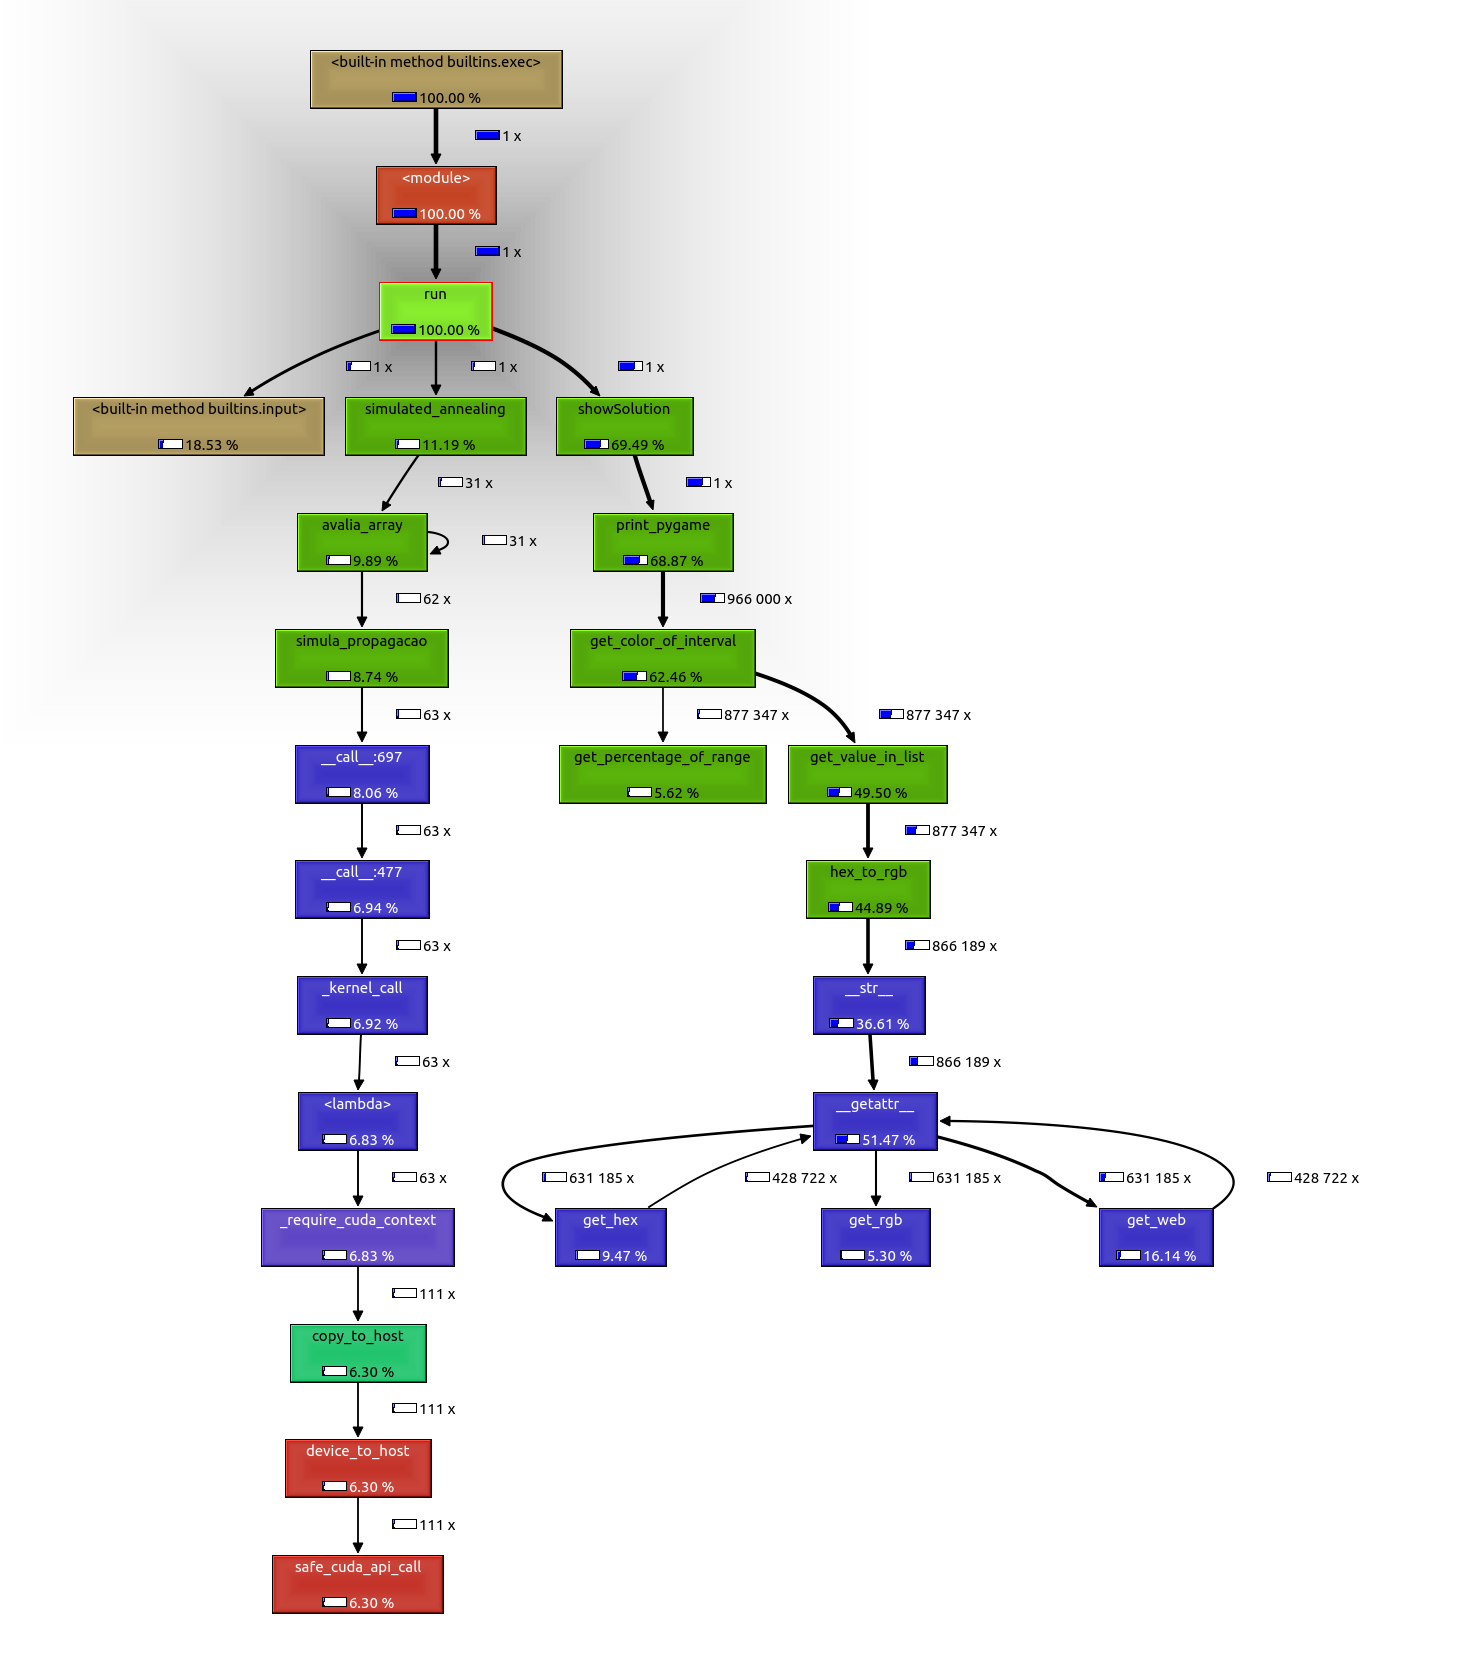
\includegraphics[scale=0.48]{imagens/graph.jpg}
    \end{center}
    \legend{Fonte: Elaboração do autor}
\end{figure}

Assim, cada retângulo do grafo da \autoref{cprofile} representa um
método implementado, sendo eles referentes aos métodos implementados
utilizando Python e aos métodos de bibliotecas utilizadas no
desenvolvimento da aplicação. Também pode ser visto que cada aresta no
grafo possui uma barra de porcentagem representando visualmente sua
fatia de tempo gasto na aplicação como num todo, juntamente com o número
de vezes que o método foi chamado podendo assim concluir que os cálculos
numéricos são realizados rapidamente e o que demanda tempo é a
representação gráfica dos dados. Para realizar a interpretação do
arquivo de saída, basta utilizar o comando \emph{pyprof2calltree -k -i
PlacementAPs.cprof} no terminal com o arquivo gerado ao fim da
simulação, nesse caso, \emph{PlacementAPs.cprof}.

\section{Paralelização em GPU}\label{paralelizauxe7uxe3o-em-gpu}

A decisão de fazer uso da GPU para ajudar no desempenho foi eficiente. A
transição de um código sequencial para um código paralelizado foi feita
aos poucos. No início, foi importado da biblioteca numba o módulo
\emph{jit} e adicionado sob todos os cabeçalhos dos métodos a anotação
\emph{@jit}. Apenas com isso, o código será compilado em código de
máquina no momento que for executado (\emph{just-in-time}). Abaixo é
possível ver um exemplo de um método que será compilado para código de
máquina utilizando a anotação \emph{@jit}:

\lstinputlisting[language=Python]{code/calc_distance.py}

Após utilizar as anotações nos métodos, foi escolhido o método que
demandava mais recursos e demandava todo o tempo. Utilizando o resultado
obtido pelo Profile, foi possível ver que o método era o que realizava a
avaliação da solução em ponto dentro do \emph{Simulated Annealing}.
Neste momento, o método calcula a intensidade do sinal para cada ponto
da matriz e, para cada ponto, calcula a absorção das paredes,
percorrendo uma lista com todas as paredes do ambiente. Quanto maior o
detalhamento do ambiente, mais linhas o ambiente terá e maior será a
lista de paredes a se verificar absorções.

Posteriormente à decisão do método a deixar a cargo da GPU realizar os
cálculos, todo o código foi transcrito de forma a dividir todo o
trabalho entre os núcleos de CUDA disponíveis. No código abaixo é
possível ver, no método que realiza a propagação do sinal, que uma
matriz utilizando a biblioteca numpy é criada, as dimensões dos
\emph{blocks} e \emph{grids} (os valores foram escolhidos empiricamente,
dependem do hardware utilizado e do problema a ser trabalhado). Logo
após, a matriz é enviada para a GPU para ser compartilhada entre
\emph{blocks} e \emph{threads}. O método que realiza o cálculo da
intensidade do sinal é chamado de acordo com os \emph{blocks} e
\emph{grids} definidos. Então, a matriz que foi enviada para a GPU é
trazida de volta e retornada para continuar com os cálculos.

\lstinputlisting[language=Python]{code/simula_propagacao_gpu.py}

Na \autoref{grid_blocks} é possível compreender facilmente como é a
divisão dos \emph{blocks}, \emph{grids} e \emph{threads}.

\begin{figure}[ht]
    \caption{\label{grid_blocks} Divisão interna da GPU dos blocks, grids e threads}
    \begin{center}
        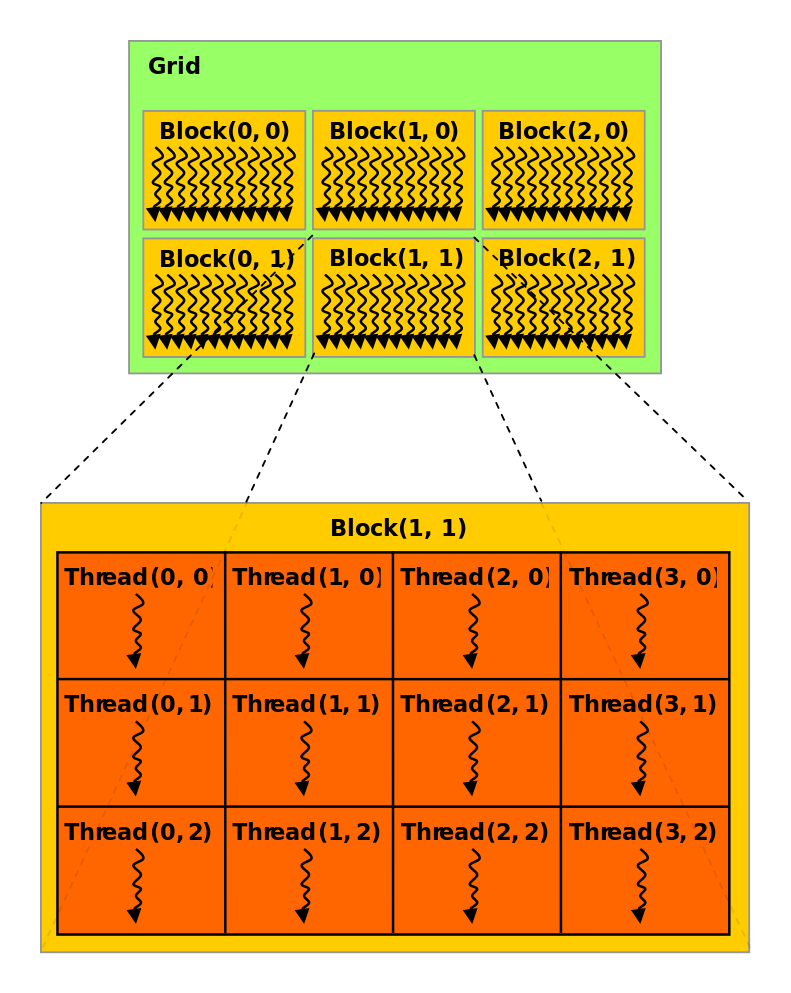
\includegraphics[scale=0.4]{imagens/block-grid.jpg}
    \end{center}
    \legend{Fonte: \url{https://en.wikipedia.org/wiki/Thread_block}}
\end{figure}

O equipamento utilizado para o desenvolvimento utiliza uma placa de
vídeo NVIDIA modelo GeForce GT 740M\footnote{Disponível em
  \url{https://www.geforce.com/hardware/notebook-gpus/geforce-gt-740m}.
  Acesso em: 29 out. 2017.} com 2GB de memória dedicada; possui 384
núcleos CUDA, com um clock básico de 993 MHz, 1300 milhões de
transistores e com vazão do barramento PCIe de até 80 Gb/s.

O método ``\emph{simulate\_kernel\_gpu}'' foi escolhido para trabalhar
com a matriz de propagação. Nele, a matriz é percorrida de acordo com os
valores dos \emph{blocks} e \emph{grids} informados no método anterior.
Para cada célula da matriz é executado o método
``\emph{propagation\_model\_gpu}'', o qual, segundo o próprio nome já
diz, realiza o cálculo do modelo de propagação utilizando a GPU e está
diretamente ligado ao ``\emph{propagation\_model}'' que obtém valores do
modelo de propagação e os miliwatts a serem subtraídos do cálculo da
perda por paredes. O código referente ao
``\emph{simulate\_kernel\_gpu}'' pode ser visto abaixo.

\lstinputlisting[language=Python]{code/simulate_kernel.py}

O cálculo do valor do sinal naquele ponto é \(O(k)\) pois consiste em um
operação envolvendo multiplicação, divisão, exponenciação/logaritmo,
portanto, assintoticamente é: \(O(1)\). Em cada simulação deve-se
calcular o valor para a propagação em cada ponto de uma matriz \(NxM\).
Considerando que uma das dimensões é maior que a outra, podemos dizer
que o custo é \(NxN\): \(O(n^{2})\) e \(O(1\times n^{2}) = O(n^{2})\)
para aplicar a operação em todos os pontos da matriz. Mas, entre cada
ponto da matriz (PM) e o AP, podem haver \(k\) paredes, que deve-se
verificar se há ou não interseção entre a reta AP-PM e a reta formada
pela parede. Tal operação, utilizando a fórmula de geometria analítica
para interseção de retas, custa \(O(1)\) para cada parede e
\(k\times O(1)\) para verificar cada parede. Como \(k\) é
suficientemente grande em relação a \(n\), podemos considerar o custo de
verificar se há interseção com paredes como \(O(n)\). Para fazer essa
verificação de cada parede para cada ponto da Matriz, temos então:
\(O(n)\times O(n^{2}) = O(n^{3})\).

Quanto ao \emph{Simulated Annealing} (SA), a cada rodada ele aleatoriza
uma solução vizinha (\(v\)) e avalia-a (\(fo\)), e como o SA tem uma
quantidade finita e decremental de iterações em função do fator de
resfriamento, a quantidade de vizinhos explorados é em torno de
\(v = log(n)\). Assim, a complexidade do SA é em torno de \(O(fo*v)\),
ou seja: \(O(fo \times log n)\). Como a função objetivo \((fo)\) consome
\(O(n^{3})\), teríamos: \(O(n^{3} * log n)\).

É importante notar que a anotação deste método é diferente das demais
que utilizam o \emph{@jit} para gerar código de máquina. A anotação
\emph{@jit} é o caminho geral do compilador, que pode ser orientado
opcionalmente para um dispositivo CUDA. A anotação \emph{@cuda.jit} é
efetivamente o dialeto de núcleo de mais baixo nível do CUDA para Python
que a empresa \emph{Continuous Analytics} desenvolveu. Assim é possível
receber suporte para variáveis embutidas do CUDA como o \emph{threadIdx}
e especificadores de espaço de memória compartilhada. Caso seja
necessário escrever um \emph{kernel} CUDA (como o método
\emph{simulate\_kernel\_gpu}) em Python e compilá-lo e executá-lo (como
ocorreu nesse caso), deve-se usar a anotação \emph{@cuda.jit}. Caso
contrário, se for necessário apenas acelerar algum método existente,
deve-se usar somente \emph{@jit} com uma anotação alvo do CUDA.

\section{Validação dos modelos}\label{validauxe7uxe3o-dos-modelos}

Durante e após a implementação dos modelos de perda e atenuação do sinal
\emph{wireless} e modelagem de propagação dos sinais pelo ambiente,
foram comparados os resultados da simulação com o resultado real
esperado. Para tal, pode-se utilizar o atual posicionamento dos APs
Wi-Fi no campus e realizar experimentos de \emph{Wireless Site Survey},
ou seja, medições reais da intensidade de sinal em determinados pontos
do ambiente analisado.

Tais resultados foram então comparados e podem ser visto com a
\autoref{captura} e a \autoref{simulacao_vinicius} com os resultados
previstos pela simulação (através da visualização gráfica da propagação
no ambiente), para que os modelos de propagação e características do
modelo espacial pudessem ser calibrados, num processo de melhoria
contínua visando ao aumento da precisão da solução a ser apresentada. É
válido reiterar que os parâmetros do \emph{Simulated Annealing} e da
função \emph{NP-Log} foram calibrados para melhor representar o ambiente
do IFMG \emph{campus} Formiga, de acordo com seus materiais de
construção, espessura de suas paredes, pisos e teto.

\begin{figure}[ht]
    \caption{\label{captura} Captura realizada no Bloco C, para um AP "18:8B:9D:69:E8:B2" posicionado em (x=660,y=260) e irradiando no Canal 11 (2.462 GHz).}
    \begin{center}
        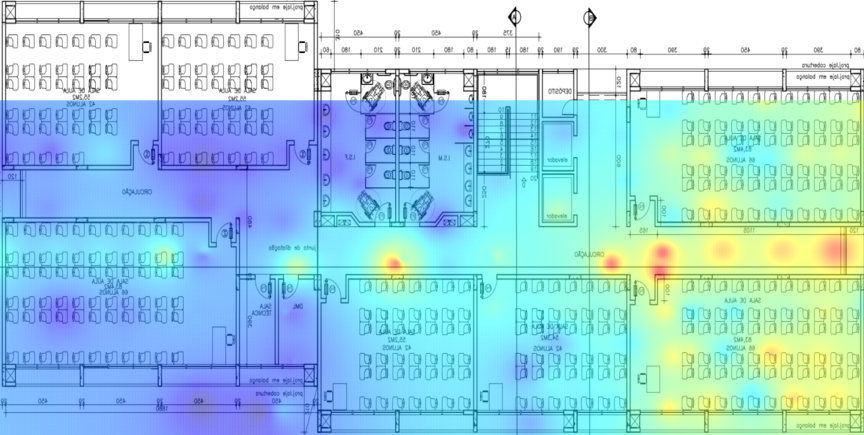
\includegraphics[scale=0.5]{imagens/captura.jpg}
    \end{center}
    \legend{Fonte: \cite{VINICIUS}}
\end{figure}
\begin{figure}[ht]
    \caption{\label{simulacao_vinicius} Simulação realizada com dados empíricos nas mesmas configurações do bloco C. }
    \begin{center}
        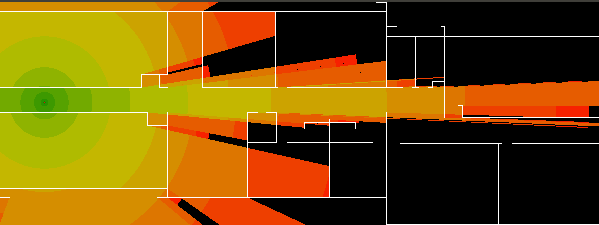
\includegraphics[scale=0.7]{imagens/simulacao_vinicius.png}
    \end{center}
    \legend{Fonte: Elaboração do autor}
\end{figure}

Assim é possível ver como é notável a aplicação de que os modelos
físicos teóricos obtiveram o comportamento relativamente parecido com a
coleta e simulação realizada empiricamente, fazendo com que o modelo
utilizado esteja realmente validado com a realidade.

\chapter{RESULTADOS E ANÁLISE}\label{resultados-e-anuxe1lise}

Neste capítulo serão mostrados os resultados obtidos a partir da
implementação de toda a fundamentação teórica e a explicação dos
procedimentos desenvolvidos. Será apresentada também uma análise de
custo computacional e um ajuste de curvas utilizando os softwares
\emph{cProfile} e o \emph{R-Project}, respectivamente.

\section{\texorpdfstring{Simulação da propagação de sinais
\emph{wireless}}{Simulação da propagação de sinais wireless}}\label{simulauxe7uxe3o-da-propagauxe7uxe3o-de-sinais-wireless}

As primeiras simulações gráficas realizadas tiveram como objetivo apenas
exibir o comportamento do espectro do sinal \emph{Wi-Fi}, considerando
tanto o seu decaimento com a distância quanto sua absorção pelas
paredes, assim, demonstrar graficamente o seu valor dentro da matriz de
propagação. A \autoref{captura_inicial} mostra a simulação da propagação
de sinais de \emph{microondas} na planta baixa do bloco A do IFMG
\emph{campus} Formiga. Para a obtenção de tal resultado da simulação e
dos próximos resultados que serão mostrados neste capítulo, foi
utilizado o código em Python\footnote{\url{https://github.com/samuelterra22/tcc/blob/master/PlacementAPs.py}}
que faz uso da GPU.

\begin{figure}[ht]
    \caption{\label{captura_inicial} Simulação da propagação de sinais de microondas no edifício utilizando versão inicial do algoritmo. }
    \begin{center}
        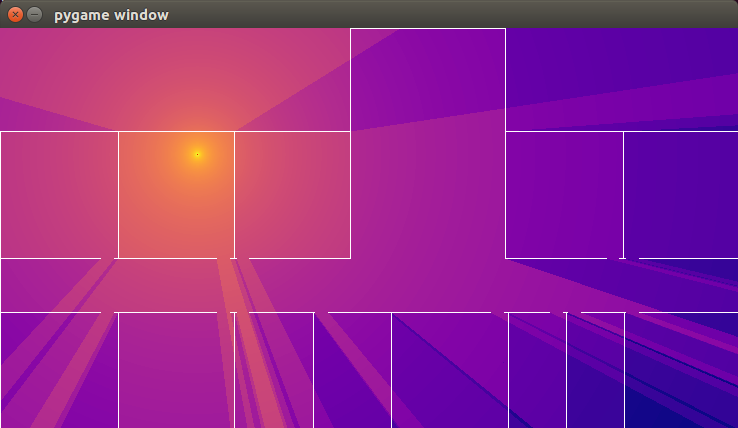
\includegraphics[scale=0.6]{imagens/captura-inicial.jpg}
    \end{center}
    \legend{Fonte: Elaboração do autor}
\end{figure}

Na \autoref{capturas} tem-se quatro capturas, nas quais as imagens
\emph{(a)}, \emph{(b)} e \emph{(d)} não possuem as portas ou janelas
implementadas, ou seja, os cômodos são tratados como ambientes fechados.
Já a captura \emph{(c)}, por sua vez, possui o resultado gráfico da
simulação e tem aberturas nas paredes, simulando as portas. Observe que
quanto maior é o número de paredes, com a atenuação do sinal,
sombreamentos são criados.

\begin{figure}[htb]
    
    \caption{\label{capturas} Simulação da propagação inicial de sinais de microondas utilizando versão inicial do algoritmo.}
    \centering
    \begin{minipage}{0.4\textwidth}
        \centering \label{captura_1}
        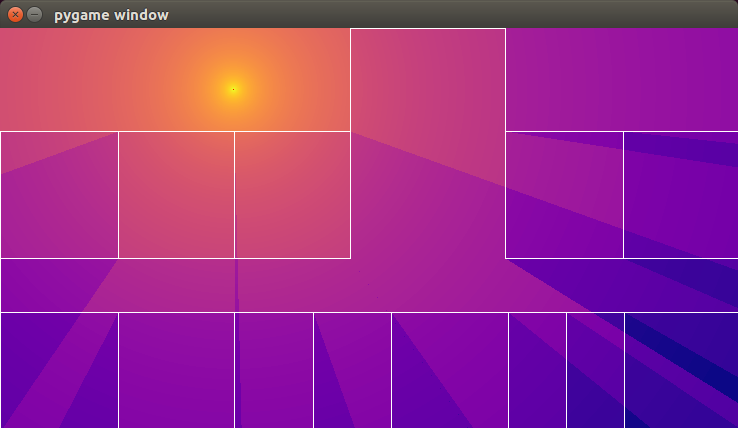
\includegraphics[scale=0.28]{imagens/captura-1.jpg}
        \legend{(a)}
    \end{minipage}
    \hfill
    \begin{minipage}{0.4\textwidth}
        \centering \label{captura_2}
        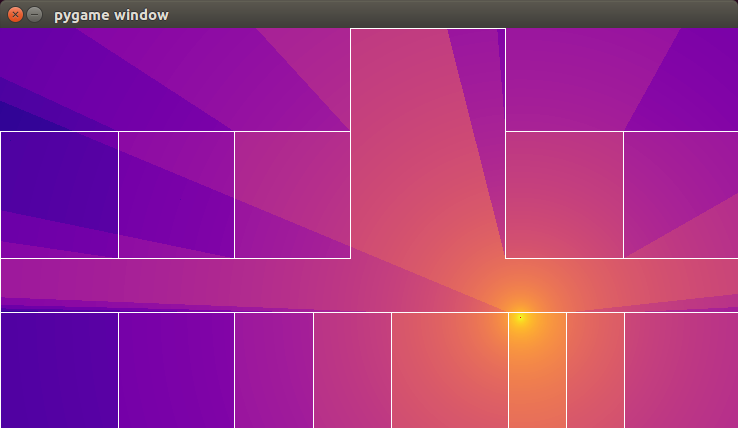
\includegraphics[scale=0.28]{imagens/captura-2.jpg}
        \legend{(b)}
    \end{minipage}
    \hfill
    \begin{minipage}{0.4\textwidth}
        \centering \label{captura_3}
        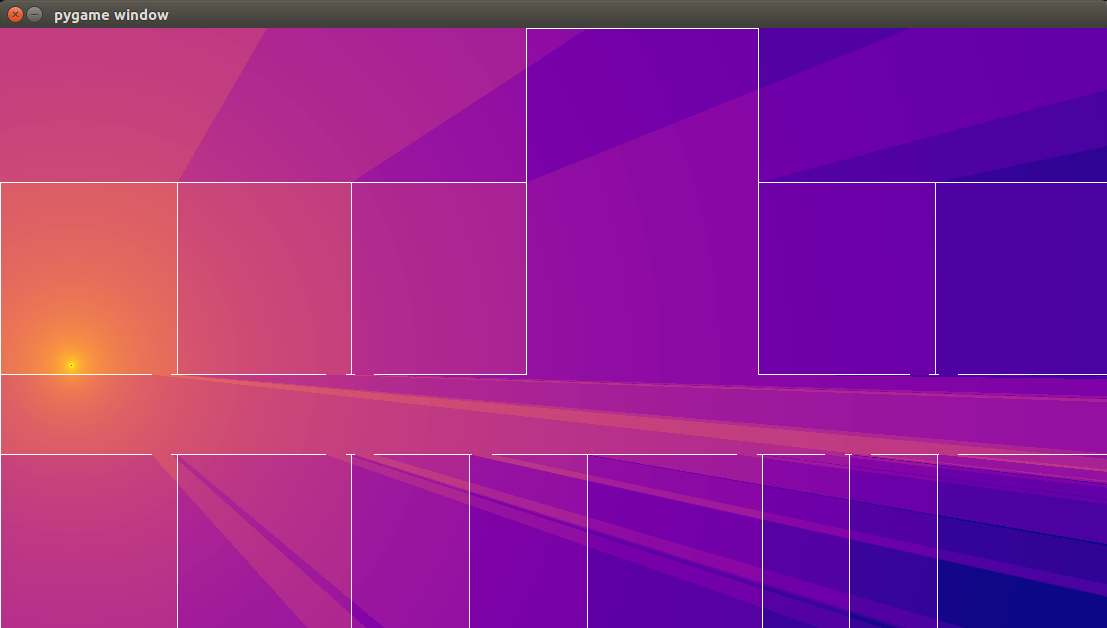
\includegraphics[scale=0.188]{imagens/captura-3.jpg}
        \legend{(c)}
    \end{minipage}
    \hfill
    \begin{minipage}{0.4\textwidth}
        \centering \label{captura_4}
        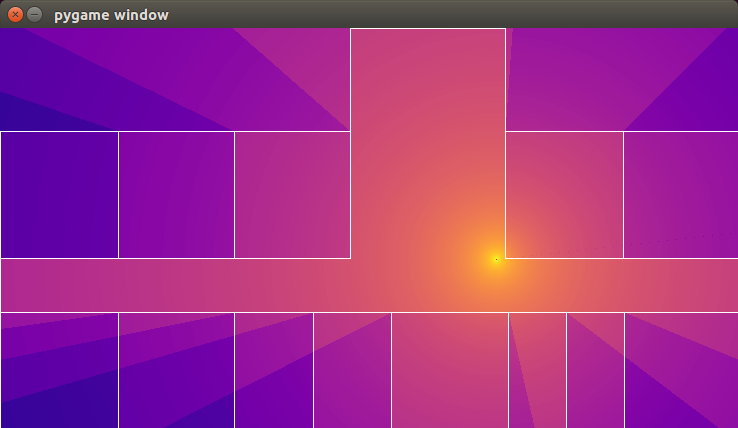
\includegraphics[scale=0.28]{imagens/captura-4.jpg}
        \legend{(d)}
    \end{minipage}

    \legend{Fonte: Elaboração do autor}
\end{figure}

Com a execução do algoritmo, além de se ter a representação gráfica do
ambiente através do PyGame, as informações da configuração da execução,
tais como os resultados, são impressos no terminal. Abaixo é possível
ver como é chamado o algoritmo e uma saída de exemplo dos dados.

\begin{lstlisting}[language=bash]
    $ python PlacementAPs.py 

    Simulando ambiente com:         400 x 149 pixels
    Escala de simulacao:            1 px : 0.1275 metros
    Quantidade de APs:              2
    Potencia de cada APs:           -25 $dB$
    FO global best: 5.762e+02

    COBERTURA DE SINAL WI-FI:
    87.62%   com boa cobertura (sinal forte)
    12.38%   de zonas de sombra (abaixo da sensibilidade)

    Cobertura por FAIXAS de intensidade de sinal
    sinal Otimo     24.3%
    sinal Bom       26.3%
    sinal Ruim      37.0%

\end{lstlisting}

Ainda com a saída de dados, ao fim da execução da otimização da posição
dos APs, é gerado um gráfico utilizando a biblioteca
\emph{matplotlib.pyplot} do Python. Com o gráfico mostrado na
\autoref{comportamento_fo}, é possível ver claramente como a função
objetivo da metaheurística se comportou durante a busca pelo espaço de
soluções. Observe que, com os seus altos e baixos, o Simulated Annealing
fugiu de seus ótimos locais e, no final da execução, retornou à sua
melhor avaliação.

\begin{figure}[ht]
    \caption{\label{comportamento_fo} Comportamento da função objetivo do Simulated Annealing na busca do melhor ponto}
    \begin{center}
        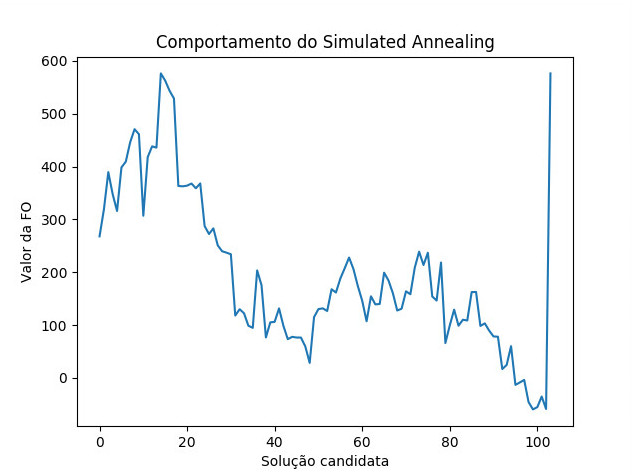
\includegraphics[scale=0.5]{imagens/comportamento-fo.jpg}
    \end{center}
    \legend{Fonte: Elaboração do autor}
\end{figure}

Neste sentido, é importante ressaltar que a \autoref{captura_inicial} e
a \autoref{capturas} representam os resultados dos primeiros testes
executados. O gradiente de cores utilizada foi o plasma, variando das
cores laranja até o azul escuro. Na próxima seção mostraremos os
resultados de testes efetuados utilizando ainda um \emph{access point}
com uma nova escala de cores, mais ainda apropriada a interpretação
imediata do que seria um sinal ótimo, bom e ruim.

\section{\texorpdfstring{\emph{Wi-Fi Placement} para 1
AP}{Wi-Fi Placement para 1 AP}}\label{wi-fi-placement-para-1-ap}

A \autoref{prop_bloco_a}, se comparada com as figuras do tópico
anterior, possuem cores mais intuitivas para os resultados obtidos, além
de uma restrição na parte gráfica, destacada com a cor preta nas áreas
onde o sinal é menor que a sensibilidade típica de um equipamento
\emph{Wi-Fi} (seja ele um computador ou AP).

\begin{figure}[ht]
    \caption{\label{prop_bloco_a} Simulação da propagação de sinais de microondas no bloco A utilizando 1 AP, sua absorção e limiar de sensibilidade.}
    \begin{center}
        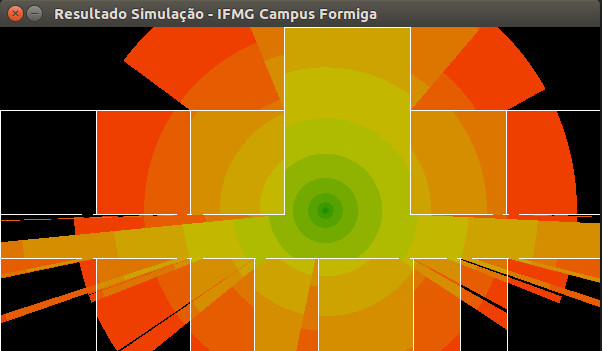
\includegraphics[scale=0.7]{imagens/prop-bloco-a-2.jpg}
    \end{center}
    \legend{Fonte: Elaboração do autor}
\end{figure}

É possível notar que o SA definiu como um caso ótimo, nesta situação, um
ponto próximo ao meio da planta. Com a posição escolhida, a cobertura do
sinal se propaga em áreas próximas à biblioteca e sala de estudo, que
contém o maior fluxo de pessoas neste bloco que utilizam o acesso à
internet. Na \autoref{prop_bloco_a}, os pontos que deixam a desejar
corresponde à potência máxima que consegue transmitir, neste caso, -25
\(dB\).

Como resultado disponibilizados via terminal, temos:

\begin{lstlisting}[language=bash]
    $ python PlacementAPs.py 
    
    Simulando ambiente com:                 600 x 325 pixels
    Escala de simulacao:                    1 px : 0.0800 metros
    Quantidade de APs:                      1
    Potencia de cada APs:                   -25 $dB$
    
    FO global best: 4.432e+02
    
    COBERTURA DE SINAL WI-FI:
    74.32%   com boa cobertura (sinal forte)
    25.68%   de zonas de sombra (abaixo da sensibilidade)
    
    Cobertura por FAIXAS de intensidade de sinal
    sinal Otimo     15.8%
    sinal Bom       26.0%
    sinal Ruim      32.5%

\end{lstlisting}

Com a \autoref{percent_2_aps_bloco_c} podemos analizar, em forma de
gráfico de pizza, a solução dada pelo algoritmo ao realizar a simulação
com dois APs no bloco A, com cada fatia correspondendo à qualidade do
sinal propagado. Observe que as zonas de sombra (sem cobertura do sinal)
tiveram uma fatia correspondente com mais de um quarto de todo o espaço
e, se somado com o sinal ruim, mais da metade da área não será atendida
com uma boa qualidade de serviço.

\begin{figure}[ht]
    \caption{\label{percent_2_aps_bloco_c} Interpretação em forma de gráfico de pizza do resultado dado para a otimização
     de dois $access points$ no bloco A.}
    \begin{center}
        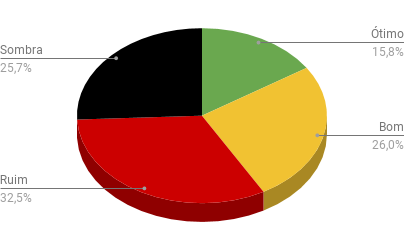
\includegraphics[scale=0.7]{imagens/prop-bloco-percent-a-2.png}
    \end{center}
    \legend{Fonte: Elaboração do autor}
\end{figure}

As plantas dos pisos 1, 2 e 3 do bloco C foram obtidas em formato DWG e
convertidas para o formato \emph{.dxf} ao final da implementação. Tais
arquivos foram simulados e obtidas suas representações gráficas. A
\autoref{captura_zona} mostra a simulação da planta baixa no bloco C
utilizando 1 AP com potência de transmissão de -25 \(dB\).

\begin{figure}[ht]
    \caption{\label{captura_zona} Simulação da propagação de sinais de microondas no bloco C utilizando 1 AP.
        }
    \begin{center}
        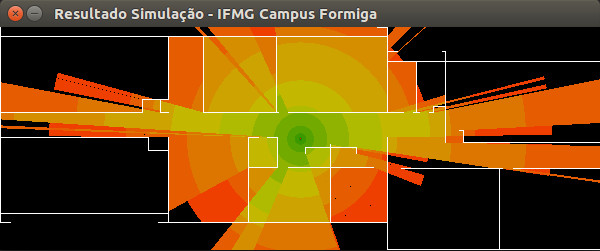
\includegraphics[scale=0.7]{imagens/captura-zona-2.jpg}
    \end{center}
    \legend{Fonte: Elaboração do autor}
\end{figure}

A saída via terminal é a seguinte:

\begin{lstlisting}[language=bash]
    $ python PlacementAPs.py 
    
    Simulando ambiente com:                 600 x 223 pixels
    Escala de simulacao:                    1 px : 0.0850 metros
    Quantidade de APs:                      1
    Potencia de cada APs:                   -25 $dB$
    
    FO global best: 2.089e+02
    
    COBERTURA DE SINAL WI-FI:
    50.89%   com boa cobertura (sinal forte)
    49.11%   de zonas de sombra (abaixo da sensibilidade)
    
    Cobertura por FAIXAS de intensidade de sinal
    sinal Otimo     11.4%
    sinal Bom       14.5%
    sinal Ruim      25.1%

\end{lstlisting}

Como pode ser visto na \autoref{prop_bloco_a} e na
\autoref{captura_zona}, quando utilizada a busca pelo ponto ótimo com um
\emph{access point}, ele tendeu a permanecer ao centro da planta. Com o
resultado dado para esta simulação com um AP, os cômodos mais ao centro
são bem atendidos com o sinal \emph{Wi-Fi}, mas ao contrário dos mais
afastados, não irão usufruir de uma boa qualidade de sinal e esse é
retirado da apresentação gráfica e dos cálculos da avaliação da função
objetivo. O resultado toma essa característica por não realizar uma
verificação das áreas subjetivamente mais importantes. Caso tivesse essa
funcionalidade implementada, a metaheurística poderia fazer com que o AP
cobrisse as áreas mais críticas do ponto de vista da utilização do
ambiente pelas pessoas.

\section{\texorpdfstring{\emph{Wi-Fi Placement} para 2 ou mais
APs}{Wi-Fi Placement para 2 ou mais APs}}\label{wi-fi-placement-para-2-ou-mais-aps}

Feita a propagação do sinal \emph{wireless} para um AP nos bloco A, foi
adaptada, recalibrada e avaliada a implementação da simulação com dois
\emph{access points}. A \autoref{captura_dois_aps} mostra como foi o
resultado da simulação do \emph{Wi-Fi} no piso 2 do bloco A.

\begin{figure}[ht]
    \caption{\label{captura_dois_aps} Simulação da propagação de sinais de microondas no bloco A utilizando 2 APs.
    }
    \begin{center}
        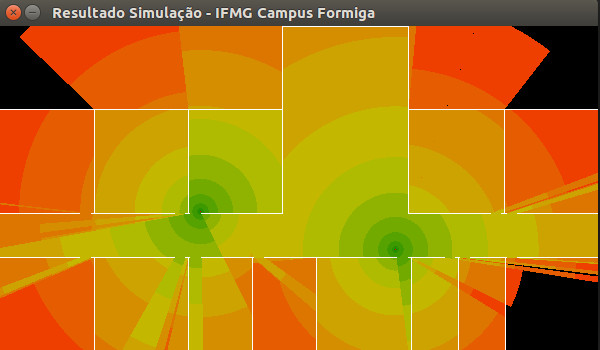
\includegraphics[scale=0.6]{imagens/captura-2-aps-2.jpg}
    \end{center}
    \legend{Fonte: Elaboração do autor}
\end{figure}

Como pode ser visto, a heurística pode então dar, como o resultado, dois
pontos que visualmente aparentam ser muito bons. Na
\autoref{captura_dois_aps} pode ser visto que os dois APs foram alocados
pela metaheurística com uma distância de folga, fazendo com que possam
aproveitar a propagação do espectro no ambiente. Com a escolha sugerida
pelo SA, utilizando um \emph{access point} transmitindo a -25 \(dB\),
pode-se também notar que algumas partes das salas nos extremos não estão
recebendo uma qualidade de sinal como na sala em que os APs estão
instalados, mas mesmo assim, a maior parte da área está recebendo sinal,
havendo poucas zonas onde a potência recebida é inferior à sensibilidade
do equipamento.

Abaixo é possível visualizar o resumo da execução do algoritmo:

\begin{lstlisting}[language=bash]
    $ python PlacementAPs.py 
    
    Simulando ambiente com:                 600 x 325 pixels
    Escala de simulacao:                    1 px : 0.0800 metros
    Quantidade de APs:                      2
    Potencia de cada APs:                   -25 $dB$
    
    FO global best: 6.112e+02
    
    COBERTURA DE SINAL WI-FI:
    91.12%   com boa cobertura (sinal forte)
    8.88%    de zonas de sombra (abaixo da sensibilidade)
    
    Cobertura por FAIXAS de intensidade de sinal
    sinal Otimo     27.1%
    sinal Bom       31.3%
    sinal Ruim      32.7%
\end{lstlisting}

O mesmo teste foi realizado com a planta baixa do bloco C, porém agora,
para que seja possível ter uma maior cobertura da área do prédio, a
simulação foi realizado com um equipamento com potência de -17 \(dB\).
Na \autoref{captura_dois_aps_c}, pode ser visto quais são os pontos
sugeridos pelo SA na busca para a alocação dos mesmos.

\begin{figure}[ht]
    \caption{\label{captura_dois_aps_c} Simulação da propagação de sinais de microondas no bloco C utilizando 2 APs.
    }
    \begin{center}
        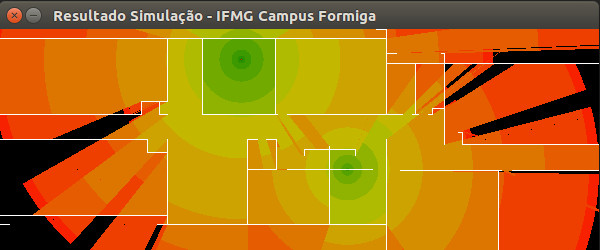
\includegraphics[scale=0.7]{imagens/captura-2-aps-bloco-c-2.jpg}
    \end{center}
    \legend{Fonte: Elaboração do autor}
\end{figure}

Com o resultado dado pelo SA no bloco C, pode-se notar que foi possível
cobrir praticamente toda a área. Tiveram algumas áreas com pontos cegos
porém, podem ser consideradas de certa forma um mal necessário quando o
objetivo é obter a maior cobertura do sinal. Um resultado ainda melhor
pode ser encontrado se for feito um maior refinamento do SA. A saída
dada pelo algoritmo é a seguinte:

\begin{lstlisting}[language=bash]
    $ python PlacementAPs.py 
    
    Simulando ambiente com:                 600 x 223 pixels
    Escala de simulacao:                    1 px : 0.0850 metros
    Quantidade de APs:                      2
    Potencia de cada APs:                   -17 $dB$
    
    COBERTURA DE SINAL WI-FI:
    89.76%   com boa cobertura (sinal forte)
    10.24%   de zonas de sombra (abaixo da sensibilidade)
    
    Cobertura por FAIXAS de intensidade de sinal
    sinal Otimo     28.4%
    sinal Bom       24.8%
    sinal Ruim      36.6%
\end{lstlisting}

A busca utilizando três \emph{access points} também foi realizada. O
resultado da propagação do sinal pode ser visto na
\autoref{captura_3_aps_bloco_c} utilizando equipamentos com potência de
transmissão de -25 \(dB\).

\begin{figure}[ht]
    \caption{\label{captura_3_aps_bloco_c} Simulação da propagação de sinais de microondas no bloco C utilizando 3 APs com potência de -25 $dB$.
    }
    \begin{center}
        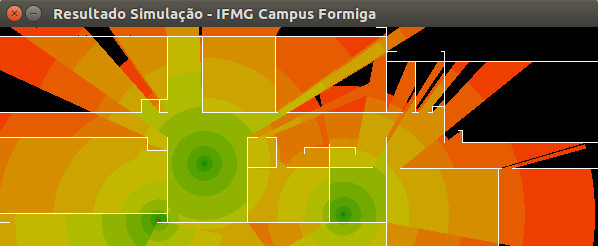
\includegraphics[scale=0.7]{imagens/captura-3-aps-bloco-c.jpg}
    \end{center}
    \legend{Fonte: Elaboração do autor}
\end{figure}

A os valores dados na saída são os seguintes:

\begin{lstlisting}[language=bash]
    $ python PlacementAPs.py 
    
    Simulando ambiente com:                 600 x 223 pixels
    Escala de simulacao:                    1 px : 0.0850 metros
    Quantidade de APs:                      3
    Potencia de cada APs:                   -25 $dB$
    
    FO global best: 5.169e+02
    
    COBERTURA DE SINAL WI-FI:
    81.69%   com boa cobertura (sinal forte)
    18.31%   de zonas de sombra (abaixo da sensibilidade)
    
    Cobertura por FAIXAS de intensidade de sinal
    sinal Otimo     25.8%
    sinal Bom       28.1%
    sinal Ruim      27.7%
\end{lstlisting}

Na \autoref{captura_3_aps_bloco_a} é possível ver propagação do sinal
utilizando 3 access points no bloco A com equipamentos transmitindo a
-25 \(dB\).

\begin{figure}[ht]
    \caption{\label{captura_3_aps_bloco_a} Simulação da propagação de sinais de microondas no bloco A utilizando 3 APs com potência de -25 $dB$.
    }
    \begin{center}
        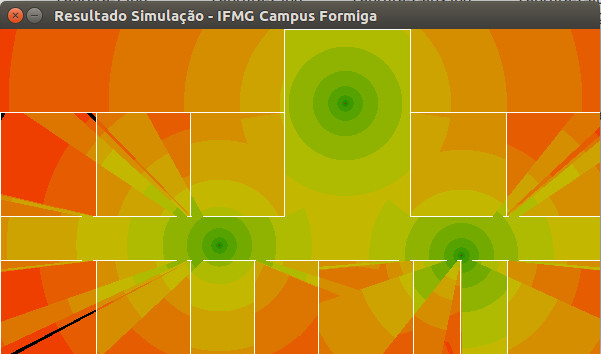
\includegraphics[scale=0.7]{imagens/captura-3-aps-bloco-a.jpg}
    \end{center}
    \legend{Fonte: Elaboração do autor}
\end{figure}

A os valores dados na saída para a simulação da
\autoref{captura_3_aps_bloco_a} com três \emph{access points} no bloco A
são os seguintes:

\begin{lstlisting}[language=bash]
    $ python PlacementAPs.py 
    
    Simulando ambiente com:          600 x 325 pixels
    Escala de simulacao:             1 px : 0.0800 metros
    Quantidade de APs:               3
    Potencia de cada APs:            -25 $dB$
    
    FO global best: 6.974e+02
    
    COBERTURA DE SINAL WI-FI:
    99.74%   com boa cobertura (sinal forte)
    0.26%    de zonas de sombra (abaixo da sensibilidade)
    
    Cobertura por FAIXAS de intensidade de sinal
    sinal Otimo     32.7%
    sinal Bom       36.6%
    sinal Ruim      30.4%
\end{lstlisting}

\chapter{CONSIDERAÇÕES FINAIS}\label{considerauxe7uxf5es-finais}

O \emph{software} desenvolvido neste trabalho é capaz de (i) receber
como entrada uma representação espacial 2D do ambiente (planta-baixa de
um piso do edifício), podendo também ser informada a posição inicial dos
APs como parâmetros adicionais para o algoritmo; (ii) realizar a
simulação da propagação dos sinais de microondas dos APs Wi-Fi pelas
dependências do edifício; (iii) aplicar a metaheurística computacional
para explorar o espaço de soluções do posicionamento de APs; (iv)
fornecer como saída a proposta de novo(s) posicionamento(s) dos APs
visando ampliar a cobertura do sinal \emph{Wi-Fi} para aquele ambiente.

O trabalho realizado foi disponibilizado de forma gratuita utilizando
Licença Pública Geral GNU --- GPL no site \emph{github.com}. Até onde
pudemos verificar, não há disponível um software livre, gratuito e de
código-fonte aberto para \emph{Wireless AP Placement}, apenas soluções
proprietárias, comerciais e custosas. Para reforçar a relevância deste
trabalho, ressaltamos que ele possibilita testar disposições de APs sem
o custo operacional de fisicamente movê-los, de maneira a propor uma
disposição espacial dos mesmos que forneça uma maior cobertura e
intensidade de sinal dentro do ambiente simulado.

Para trabalhos futuros, é necessária a realização de tratamento da
interferência entre canais \emph{Wi-Fi} no caso de utilização de mais de
quatro APs em um mesmo ambiente, além de uma coleta de dados mais
abrangente para obtenção de parâmetros mais precisos o modelo de
regressão logístico \emph{(NP-Log)}. Também, sugere-se que seja
utilizado mais de um modelo de propagação, complementando-se, visto que
aparentemente um único modelo não realiza estimativas tão boas tanto
para distâncias perto e longe. Portanto, sugere-se utilizar dois modelos
de propagação, um para perto \((1-10 m)\) e outro para mais longe
\((10-100 m)\), numa abordagem híbrida. Uma outra abordagem poderia ser
a aplicação de técnicas que envolvem simulação via \emph{Ray-Tracing},
podendo ser incluída em pesquisas posteriores. Ainda, caso haja demanda,
sugere-se a realização de simulação de propagação de sinais em ambiente
3D, com um maior aproveitamento dos recursos disponibilizados pela
biblioteca CUDA, objetivando uma maior precisão da obtenção dos pontos
cegos dentro de cômodos. Para se obter resultados que possibilitem uma
melhor busca pelos pontos de acesso para dois ou mais APs, novas
técnicas deverão ser utilizadas para o cálculo da função objetivo.

---------------------------------------------------------

% ----------------------------------------------------------
% ELEMENTOS PÓS-TEXTUAIS
% ----------------------------------------------------------
\postextual
% ----------------------------------------------------------

% ----------------------------------------------------------
% Início dos ELEMENTOS PÓS-TEXTUAIS
% ----------------------------------------------------------
\postextual
% ----------------------------------------------------------

% ----------------------------------------------------------
% Referências bibliográficas
% ----------------------------------------------------------
\bibliography{xxx-referencias}
% ----------------------------------------------------------
% Apêndices
% ----------------------------------------------------------
%% 
% Seção de apendices configurada como desativada
%% 
% ---

% ----------------------------------------------------------
% Anexos desativados: 
% Seção de anexos configurada como desativada
% ----------------------------------------------------------



\end{document}
